\documentclass[sigplan,10pt,review]{acmart}
\settopmatter{printfolios=true,printccs=true,printacmref=true}

% Enable/disable optional sections here
\newif\ifopt \optfalse

% Packages {{{
\usepackage{microtype}
\usepackage{bbm}
\usepackage{tikz}
\usetikzlibrary{calc}
\usetikzlibrary{graphs}
\usetikzlibrary{cd}
\usetikzlibrary{patterns}
\usetikzlibrary{backgrounds}
\usetikzlibrary{shapes}
\usepackage{bussproofs}
\usepackage{stmaryrd}
\usepackage{bbm}
\usepackage{soul}
\usepackage{booktabs}
% }}}

% Parameters {{{

%% Conference information
%% Supplied to authors by publisher for camera-ready submission;
%% use defaults for review submission.
%\setcopyright{none}
\acmPrice{}
\acmDOI{10.1145/3453483.3454097}
\acmYear{2021}
\copyrightyear{2021}
\acmSubmissionID{pldi21main-p596-p}
\acmISBN{978-1-4503-8391-2/21/06}
\acmConference[PLDI '21]{Proceedings of the 42nd ACM SIGPLAN International Conference on Programming Language Design and Implementation}{June 20--25, 2021}{Virtual, Canada}
\acmBooktitle{Proceedings of the 42nd ACM SIGPLAN International Conference on Programming Language Design and Implementation (PLDI '21), June 20--25, 2021, Virtual, Canada}

\bibliographystyle{ACM-Reference-Format}
%\citestyle{acmauthoryear}

\hyphenation{Comp-Cert}
\hyphenation{Comp-CertO}

\newcommand{\figsize}{\small}

\renewcommand{\figureautorefname}{Fig.}
%\renewcommand{\tableautorefname}{Tbl.}
\renewcommand{\equationautorefname}{Eqn.}
\renewcommand{\theoremautorefname}{Thm.}

% }}}

% Macros {{{
\newcommand{\kw}[1]{\ensuremath{ \mathsf{#1} }}
\newcommand{\ifr}[1]{\mathrel{[{#1}]}}
\newcommand{\que}{\circ}
\newcommand{\ans}{\bullet}
\newcommand{\vref}{\le_\kw{v}}
\newcommand{\mext}{\le_\kw{m}}
\newcommand{\refby}{\preceq}
\newcommand{\scref}{\sqsupseteq}
\newcommand{\screfd}{\sqsubseteq}
\newcommand{\CA}{{ \mathcal{C\!A} }}

% Pointers for justified sequences %{{{

% Parameters
\newcommand{\pshift}{1.6ex}
\newcommand{\pcdist}{2.5}
\newcommand{\pcangle}{60}

% Pointer hook
\newcommand{\ph}[1]{%
  \tikz[remember picture]{\coordinate (#1);}}

% Pointer to
\newcommand{\ptc}[2]{%
  \rule{0pt}{1.4em}%
  \tikz[remember picture, overlay]{
    \draw[->,#2]
      let \p{dest} = (#1),
          \n1 = {ln(veclen(\x{dest}, \y{dest}) + 1)},
          \p1 = ($(0,0)+(0,\pshift)$),
          \p4 = ($(#1)+(0,\pshift)$),
          \p2 = ($(\p1)!\n1*\pcdist!-\pcangle:(\p4)$),
          \p3 = ($(\p4)!\n1*\pcdist!+\pcangle:(\p1)$) in
        (\p1) .. controls (\p2) and (\p3) .. (\p4);}}
\newcommand{\pt}[1]{%
  \ptc{#1}{gray}}
\newcommand{\bpt}[1]}}

\ifopt
  \newcommand{\opt}[2]{#1}
  \newenvironment{optional}{\begin{color}{gray}}{\end{color}}
\else
  \newcommand{\opt}[2]{#2}
  \excludecomment{optional}
\fi
\newcommand{\anon}[2]{#1}

% TikZ setup
\pgfdeclarelayer{tint}
\pgfdeclarelayer{nodes}
\pgfsetlayers{tint,main,nodes}
\newcommand{\stens}{0.6}

% }}}

\title{CompCertO: Compiling Certified Open C Components} %{{{

\author{J\'er\'emie Koenig}
\orcid{0000-0002-3168-5925}
\affiliation{
  \institution{Yale University}
  \city{New Haven}
  \state{CT}
  \country{USA}
}
\email{jeremie.koenig@yale.edu}

\author{Zhong Shao}
\affiliation{
  \institution{Yale University}
  \city{New Haven}
  \state{CT}
  \country{USA}
}
\email{zhong.shao@yale.edu}

%}}}

\begin{document}

\begin{abstract} %{{{
Since the introduction of CompCert,
researchers have been refining
its language semantics and correctness theorem,
and used them as components
in software verification efforts.
Meanwhile,
artifacts ranging from CPU designs to network protocols
have been successfully verified,
and there is interest in
making them interoperable
to tackle end-to-end verification
at an even larger scale.

%To that end,
%\anon{it has been proposed}{we believe} that
Recent work shows that
a synthesis of existing research on
game semantics,
refinement-based methods, and
abstraction layers
has the potential to serve as a common theory
of certified components.
Integrating CompCert to such a theory
is a critical goal.
However,
the requirements we have identified for
CompCert to be deployed in this context
are not met by any of its existing variants.

CompCertO extends the correctness theorem of CompCert
to characterize compiled program components
directly in terms of their interaction with each other.
Through a careful and compositional treatment
of calling conventions,
this is achieved with minimal effort.
\end{abstract}
%}}}

%% 2012 ACM Computing Classification System (CSS) concepts
%% Generate at 'http://dl.acm.org/ccs/ccs.cfm'.
\begin{CCSXML}
<ccs2012>
   <concept>
       <concept_id>10011007.10010940.10010992.10010998.10010999</concept_id>
       <concept_desc>Software and its engineering~Software verification</concept_desc>
       <concept_significance>500</concept_significance>
       </concept>
   <concept>
       <concept_id>10003752.10010124.10010138.10010142</concept_id>
       <concept_desc>Theory of computation~Program verification</concept_desc>
       <concept_significance>500</concept_significance>
       </concept>
   <concept>
       <concept_id>10011007.10011006.10011041</concept_id>
       <concept_desc>Software and its engineering~Compilers</concept_desc>
       <concept_significance>500</concept_significance>
       </concept>
 </ccs2012>
\end{CCSXML}

\ccsdesc[500]{Software and its engineering~Software verification}
\ccsdesc[500]{Theory of computation~Program verification}
\ccsdesc[500]{Software and its engineering~Compilers}
%% End of generated code


%% Keywords
%% comma separated list
\keywords{Compositional Compiler Correctness, Game Semantics, Simulation Convention, Language Interface}  %% \keywords are mandatory in final camera-ready submission

\maketitle

\section{Introduction} %{{{

%\subsection{Large-scale verification} %{{{

Over the past decade,
researchers have been able to formally verify
%the total functional correctness of
various key components of computer systems,
including
compilers \cite{compcert, vellvm},
operating system kernels \cite{sel4,popl15},
file systems \cite{fscq} and
processor designs \cite{safe,kami}.
Building on these successes,
the research community is attempting
to construct large-scale, heterogenous certified systems
by using formal specifications as interfaces between
the correctness proofs of various components %, covering a range of abstraction levels
\cite{deepspec},
enabling the deployment of formal methods
at an unprecedented scale.

Given the importance of compilers in
the construction of present-day computer systems,
the integration of a certified compiler to any framework
attempting to tackle end-to-end verification
should be a litmus test.
However, adapting certified compilation to this context
comes with new challenges.

%}}}

\subsection{Compositional compiler correctness} %{{{

Compiler correctness is often formulated as a
\emph{semantics preservation} property,
asserting that the semantics
of the compiled program $\kw{C}(p)$
are related in some particular way
to the semantics
of the source program $p$:
\begin{equation} \label{eqn:semp}
  \llbracket p \rrbracket_\kw{S} \sim
  \llbracket \kw{C}(p) \rrbracket_\kw{T}
  \,.
\end{equation}
For whole-program compilers,
semantics preservation is straightforward enough.
In CompCert,
the semantics of the source and target programs
are given as labelled transition systems,
and the relation $\sim$ is a simulation property.
%A more abstract version of the theorem can also be derived,
%where the semantics are given in terms of observable traces,
%and correctness is expressed as a trace containment property.

However,
practical applications involve
program \emph{components} which we want to compile
and verify separately from each other.
In principle,
this can be addressed by the use of a compositional semantics,
enabling the formulation of (\ref{eqn:semp})
at the level of individual components,
but traditional approaches to compositional semantics
fare poorly in the presence of advanced language features,
or the kind of data abstraction
involved in the compilation process.
In the context of CompCert,
early attempts along these lines
have proven excessively
complex and limited \cite{cpp15,compcompcert}.

As a result,
common wisdom holds semantics preservation
to be a lost cause
for compositional compiler correctness \cite{next700}.
Instead,
research has focused on
compositional reasoning methods
based on contextual refinement,
side-stepping the need for compositional semantics preservation
\cite{sepcompcert,compcertm}.

%}}}

\subsection{Decomposing heterogenous systems} %{{{

Unfortunately,
these methods share an intrinsic limitation:
they presuppose the existence of a completed system
to be proven correct,
and compositionality only operates within its boundary.
This becomes a serious impediment
in the context of large-scale heterogeneous systems.

%Indeed, while
%CompCertM allows the user to reason about components with C and assembly
%call interfaces in isolation and link them, its top-level correctness
%theorem only characterizes closed semantics where no calls to outside
%components remain.
%The line of work we are pursuing attempts to go beyond this horizon.
%We envision a verification infrastructure where,
%for example,
%software and hardware components could be freely combined and described
%at various levels of abstraction.
%In the context of the verification of heterogenous systems
%where software and hardware component

\begin{example} \label{ex:nicdriver} %{{{
Consider the problem of verifying
a network interface card (NIC) driver.
The NIC and its driver are closely coupled,
but the details of their interaction
are irrelevant to the rest of the system;
these details should not leak into our large-scale reasoning.
Instead,
we wish to treat the NIC and driver as a unit
and establish a direct relationship between calls into
the driver's C interface and network communication.
Together, the NIC and driver implement
a specification $\sigma :
\kw{Net} \rightarrow \mathcal{C}$,
meaning they \emph{use} the interface $\kw{Net}$
modeling the network,
and \emph{provide} the interface $\mathcal{C}$
modeling C function calls.

The driver code could be specified
($\sigma_\kw{drv}$)
and verified
at the level of CompCert semantics,
whereas device I/O primitives
($\sigma_\kw{io}$)
and the NIC
($\sigma_\kw{NIC}$)
would be specified as additional components
in the context of a richer model:
\[
  \sigma_\kw{NIC} : \kw{Net} \rightarrow \kw{IO}
  \qquad
  \sigma_\kw{io} : \kw{IO} \rightarrow \mathcal{C}
  \qquad
  \sigma_\kw{drv} : \mathcal{C} \rightarrow \mathcal{C}
\]
By reasoning about their interaction,
it would be possible to establish a relationship between
the overall specification $\sigma : \kw{Net} \rightarrow \mathcal{C}$ and
the composition
$\sigma_\kw{drv} \circ \sigma_\kw{io} \circ \sigma_\kw{NIC}$.
Then a \emph{compiler of certified components}
should help us transport specifications and proofs
obtained with respect to the driver's C code
to the compiled code operating at the level of assembly
($\sigma' : \kw{Net} \rightarrow \mathcal{A}$).
\end{example}
%}}}

%This problem posed by this example is the following.
%illustrated in Fig.~\ref{fig:hetsys}.
Under existing contextual approaches,
the NIC driver can only be specified and verified in terms of
its interactions at the boundary of the C program code.
Since abstracting away from these interactions
is the role of a driver in the first place,
this is a serious limitation.

To be sure,
existing techniques could be extended
to address this specific problem.
For example,
the NIC hardware model could be brought
within the scope of the ``whole program'' being considered,
and the exchange of Ethernet packets
modeled as part of its observable behavior.

However, this approach does not scale.
Example~\ref{ex:nicdriver}
is by no means a contrived corner case.
In fact, patterns of this kind are pervasive even in more mundane situations.
Many libraries available to contemporary programmers
are used to mediate access to external resources
(network services, file systems, user interfaces).
High-level specifications
for software components of this kind
must model these resources.
It would rapidly become burdensome to expect
the verification framework
to fix in advance
the dozens or hundreads
of kinds of resources and interactions
which may be involved
in the course of verifying a large-scale system.

Fortunately,
advances in compositional semantics
offer a realistic path
to tackling problems of this kind.
In particular,
game semantics (\S\ref{sec:gamesem})
provides a general and expressive framework
to model interactions between typed components.
Recent work proposes integrating
dual nondeterminism and refinement
into this framework,
extending it with powerful mechanisms
to account for abstraction \cite{rbgs-cal}.
Formulating
a correctness theorem for CompCert
which can be used in this context
is a critical step in this direction.

%\begin{figure} \label{fig:hetsys} %{{{
%  \centering
%  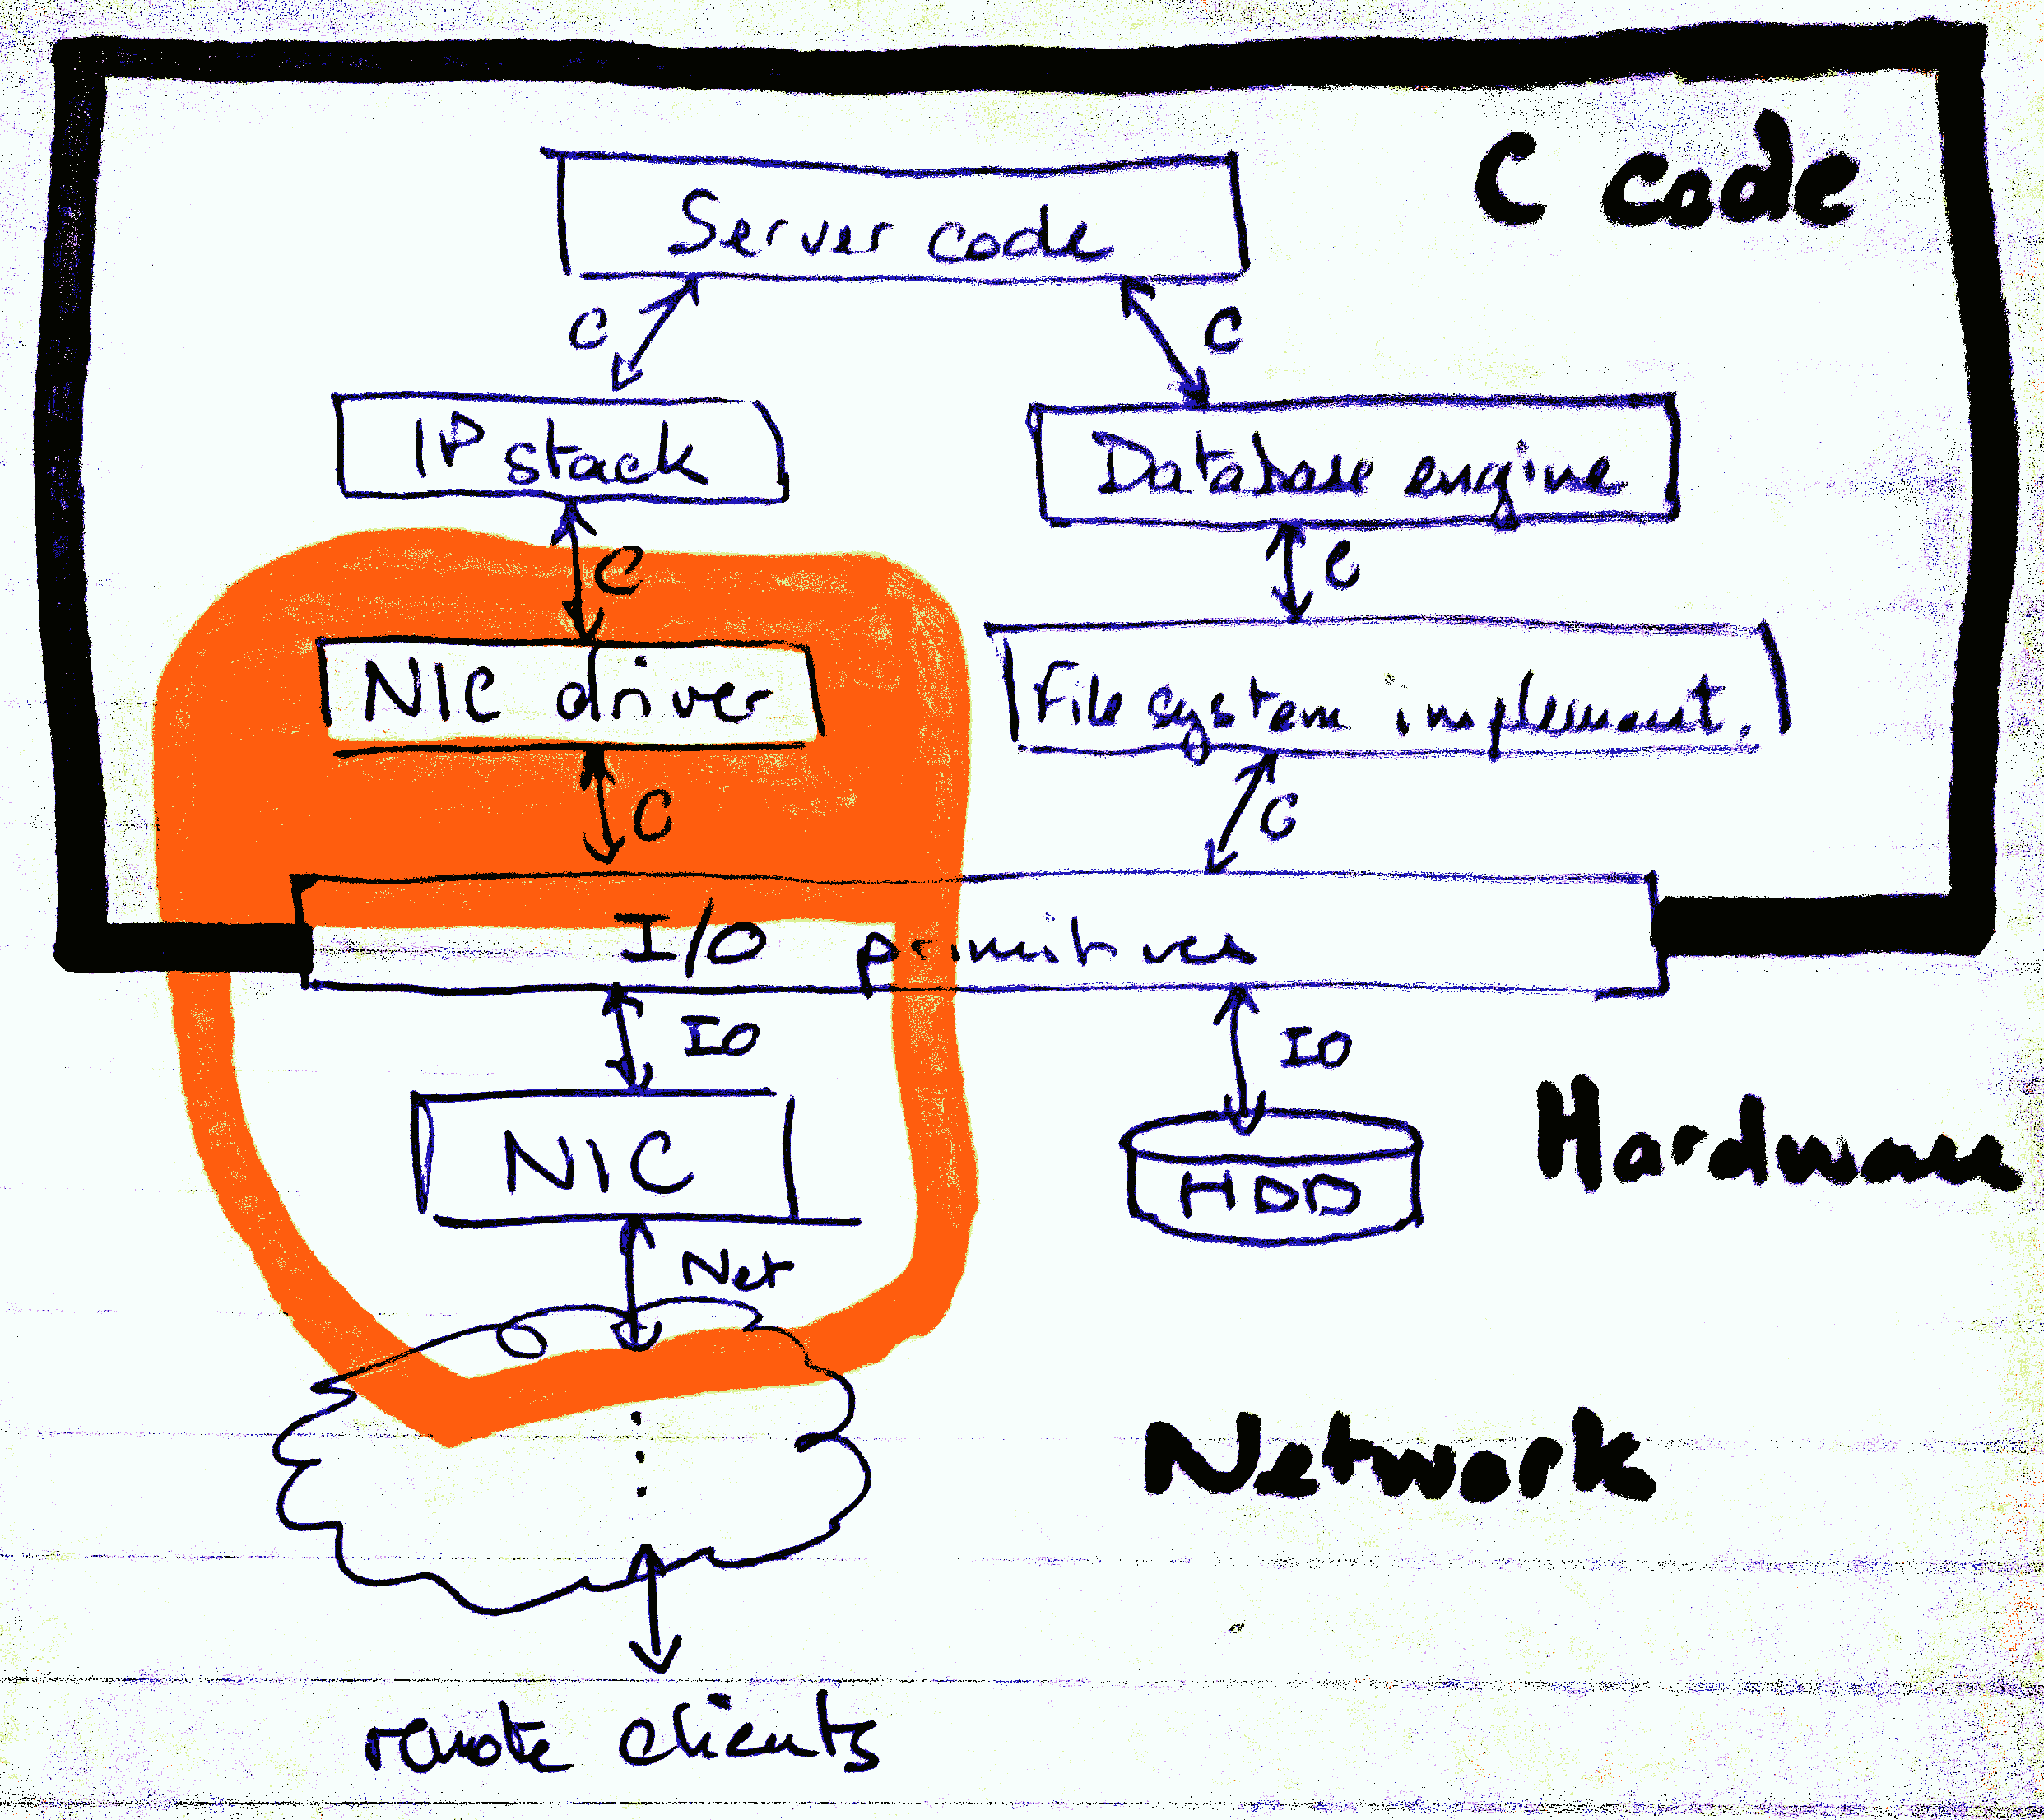
\includegraphics[scale=0.09]{hetsys}
%	\caption{A futuristic verification scenario (draft figure).
%    Contextual approaches to compositional reasoning
%    impose a boundary,
%    depicted as a thick black line,
%    between the completed program and its environment;
%    compositionality operates only within this boundary.
%    However,
%    the verification of large-scale, heterogeneous systems
%    requires modelling components which cross this boundary.}
%  \label{fig:hetsys}
%\end{figure}
%}}}

%}}}

\subsection{Contributions} \label{sec:compcertreq} %{{{

This paper introduces CompCertO,
the first extension of CompCert
satisfying the following requirements:
\begin{enumerate}
\item \label{req:opensem}
  A semantics is given for
  source and target \emph{components}.
\item \label{req:opensim}
  The correctness theorem relates
  the behaviors of corresponding
  source and target components directly.
\item \label{req:openabs}
  The C calling convention is modelled explicitly.
\item \label{req:linking}
  A form of certified component \emph{linking}
  is provided.
\item \label{req:complexity}
  Changes to existing proofs of CompCert
  are minimal.
\end{enumerate}
Each of these requirements is fulfilled
by some exisiting CompCert extension,
however none satisfies them all.

%The key to this achievement
%is the expressivity of our model.
%and our unreserved adoption of relational reasoning,
%which provides flexibility in
%describing complex phenomena
%arising from compositional compilation,
%and enables a more fine-grained separation of concerns.

We generalize CompCert semantics
to express interactions between components (\S\ref{sec:sem}),
using \emph{language interfaces}
to describe the form of these interactions
and \emph{simulation conventions}
to describe the correspondence between the interfaces
of source and target languages.
The behavior of
composite programs is specified by a
\emph{horizontal composition} operator (\S\ref{sec:sem:linker}),
which is shown to be correctly implemented
by the existing linking operator for assembly programs
(\S\ref{sec:sem:ref}).
To combine and reason about simulation proofs,
we define a notion of
\emph{CompCert Kripke logical relation} (\S\ref{sec:cklr})
and introduce a rich \emph{simulation convention algebra}.
We then use them to derive our main compiler correctness statement
from the simulation properties
of CompCertO's individual passes
(\S\ref{sec:callconv}).

%The simulation proofs for
%most of CompCert's passes
%can be updated with minimal effort.
%%In the case of more complex passes,
%Simulation conventions can be defined
%which capture the internal invariants
%used by existing proofs,
%avoiding many sources of complexity found
%in previous work.
%To facilitate reasoning about
%them, %simulation conventions,
%we define \emph{CompCert Kripke logical relations}
%(CKLR, \S\ref{sec:cklr}),
%which unify
%CompCert's memory transformations
%as structure-preserving relations
%over the memory model.
%Our treatment of invariants is presented in \S\ref{sec:inv}
%and more specialized simulation conventions
%are discussed in \S\ref{sec:backend}.

%We discuss related work in \S\ref{sec:rw}
%and %conclude with a short evaluation of
%the significance of our results in \S\ref{sec:concl}.

This paper discusses CompCertO version 0.1,
available online in the CertiKOS CompCert git repository.%
\footnote{\url{https://github.com/CertiKOS/compcert/tree/compcerto}}

%}}}

%}}}

\section{Main ideas} \label{sec:mainideas} %{{{

\begin{optional}
\subsection{Principles for system construction} \label{sec:principles} %{{{

% preamble {{{

The goal of certified system design is
to create a formal description of
the system to be constructed (the program),
while ensuring
through careful analysis
that the system
will behave properly.
To this end,
we assign
to every system $p \in P$
a mathematical object $\llbracket p \rrbracket \in \mathbb{D}$
representing its behavior.
We will call the set $\mathbb{D}$ a \emph{semantic domain}.
In this section we elucidate
the structure and properties of $\mathbb{D}$
necessary to the process of builing
large-scale certified systems.

%}}}

\paragraph{Specifications and refinement} %{{{

System design starts with a set of requirements
on the behavior of the system to be constructed
(the specification).
These requirements do not capture every detail
of the eventual system,
but delineate a range of acceptable behaviors.

In refinement-based approaches,
programs and specifications are interpreted in the same
semantic domain $\mathbb{D}$,
which is equipped with a \emph{refinement} preorder
${\refby} \subseteq \mathbb{D} \times \mathbb{D}$.
The proposition $\sigma_1 \refby \sigma_2$
asserts that $\sigma_2$ is a refinement of $\sigma_1$,
and in particular a system description $p \in P$ is a correct implementation
of $\sigma \in \mathbb{D}$ when
$\sigma \refby \llbracket p \rrbracket$.

%}}}

\paragraph{Compositionality} %{{{

Complex systems are built by assembling components
whose behavior is understood,
such that their interaction achieves a desired effect.
The syntactic constructions of
the language used to describe systems
correspond to the ways in which they can be composed.

To enable compositional reasoning,
a suitable model must provide an account of
the behavior of the composite system
in terms of the behavior of its parts.
For instance,
if the language contains a binary operator
${+} : P \times P \rightarrow P$,
then the semantic domain should be equipped with
a corresponding operation
${\oplus} : \mathbb{D} \times \mathbb{D} \rightarrow \mathbb{D}$
such that
$\llbracket p_1 + p_2 \rrbracket =
 \llbracket p_1 \rrbracket \oplus \llbracket p_2 \rrbracket$.

%}}}

\paragraph{Monotonicity} %{{{

Once a component has been shown to conform to a given specification,
we want to abstract it as a ``black box''
so that further reasoning can be done in terms of
the component's specification rather than its implementation details.
To support this,
we must establish that semantic composition operators
are compatible with refinement:
\[ \sigma_1 \refby \sigma_1' \wedge
   \sigma_2 \refby \sigma_2' \Rightarrow
   \sigma_1 \oplus \sigma_2 \refby \sigma_1' \oplus \sigma_2' \,. \]
Suppose we have two components $p_1$ and $p_2$,
where $p_2$ relies on $p_1$ for its operation,
and we want to verify that their combination $p_1 + p_2$
satisfies a specification $\sigma$.
Once we verify $p_1$ against its own specification
$\sigma_1 \refby \llbracket p_1 \rrbracket$,
by the monotonicity of ${\oplus}$ it is sufficient to show that
$\sigma \refby \sigma_1 \oplus \llbracket p_2 \rrbracket$:
\[
   \sigma \:\refby\:
   \sigma_1 \oplus \llbracket p_2 \rrbracket \:\refby\:
   \llbracket p_1 \rrbracket \oplus \llbracket p_2 \rrbracket \:=\:
   \llbracket p_1 + p_2 \rrbracket
\]

%}}}

\paragraph{Abstraction} %{{{

Large-scale systems operate across multiple layers of abstraction.
Each abstraction layer defines its own understanding of the interaction
between a component and its environment.
To relate abstraction layers we need to give
an explicit account of how their formulations of the interaction
correspond to one another.
In this work we address this by defining a heterogenous version
of the refinement relation
${\refby_\mathbb{R}} \subseteq
 \mathbb{D}_1 \times \mathbb{D}_2$ between
the abstract domain $\mathbb{D}_1$ and
the more concrete one $\mathbb{D}_2$, where
$\mathbb{R}$ specifies a correspondence between
the two views of the system.

%In related work we show that for a sufficiently general
%semantic domain, the simulation convention $\mathbb{R}$
%defines a Galois connection
%$(\mathbb{D}^\sharp, {\refby})
% \galois{\gamma}{\alpha}
% (\mathbb{D}^\natural, {\refby})$
%between the abstract and concrete domains,
%which allows refinement properties to be transferred between
%the abstract and concrete domains through the defining property
%$
%    \gamma(\sigma^\sharp) \refby \sigma^\natural \Leftrightarrow
%    \sigma^\sharp \refby \alpha(\sigma^\natural)
%$.

%}}}

%\paragraph{Compilers} %{{{
%
%This is particularly relevant
%in the context of compilers.
%Between C and assembly,
%interactions across compilation units
%are understood very differently.
%At the level of C,
%cross-module interaction is defined in terms of
%function calls;
%invoking a function consists of assigning values
%to the function's parameters,
%initializing a new stack frame,
%and finally executing the function's body.
%At the assembly level, cross-module
%interactions simply consist in branching to an address
%outside the current module with
%a certain register state.
%
%In that context,
%the correpondance between the source and target semantic domains
%depends on the \emph{calling convention} used by the compiler.
%The correctness property of a C-to-assembly compiler
%can then be stated as:
%\[ \llbracket p \rrbracket_s \sqsubseteq_\mathbb{R}
%   \llbracket C(p) \rrbracket_t \,. \]
%where
%$p$ is the source program, $C(p)$ the compiler's output,
%$\llbracket - \rrbracket_s$ gives the semantics of the source language,
%$\llbracket - \rrbracket_t$ gives the semantics of the target language,
%and $\mathbb{R}$ formalizes the C calling convention.
%
%%}}}

%}}}
\end{optional}

\subsection{Game semantics} \label{sec:gamesem} %{{{

% preamble {{{

Game semantics is a form of denotational semantics which
incorporates some operational aspects.
%An early success of this approach was
%the formulation of the first fully abstract models
%of the programming language PCF \cite{pcfajm,pcfho}.
%In this section,
%we give an overview of this line of research
%and how it can be applied in the context of CompCert.
Typically,
game semantics interpret
types as two-player games
and terms as strategies for these games.
Games describe the form of the interaction
between a program component %of the corresponding type
(the \emph{system})
and its execution context
(the \emph{environment}).
Strategies
specify which move the system plays
at each position in the game.

Positions are usually identified with sequences of moves,
and strategies with the set of positions
a component can reach.
% depending on the possible behaviors of the environment
This representation makes
game semantics similar to
the trace semantics of process algebras,
but game semantics is distinguished
by a strong polarization between
actions of the system and the environment,
and between outputs and inputs.
This confers an inherent ``rely-guarantee'' flavor
to games which facilitates compositional reasoning
\cite{cspgs}.

%}}}

\paragraph{Games} \label{sec:mainideas:gs:games} %{{{

A game is defined by a set of moves
players will choose from,
as well as a stipulation of which
sequences of moves are valid.
We focus on two-player, alternating games
where the environment plays first and
where the players
each contribute every other move.

When typesetting examples,
we underline the moves of the system.
For chess,
moves are taken in the set $\{a1 \ldots h8\} \times \{a1 \ldots h8\}$,
and a valid sequence of moves may look like:
\[ e2e4 \cdot \underline{c7c5} \cdot c2c3 \cdot \underline{d7d5} \cdots \]
The games we use to model low-level components
will rely on the following constructions.

%Most game semantics
%include additional structure
%in the description of games.
%The set of moves is usually partitioned
%into proponent and opponent moves ($M = M^\kw{O} \uplus M^\kw{P}$),
%and into questions and answers ($M = M^\que \uplus M^\ans$).
%Game models for high-order languages are often more complex.

%}}}

\paragraph{Type structure} \label{sec:mainideas:gs:types} %{{{

%While the game $\mathcal{C}$
%is extremely simple,
The expressive power of game semantics
comes from the ways in which complex games can be derived from simple ones,
and used to interpret compound types.
For example,
in the game $A \times B$
the environment initially chooses whether to play
an instance of $A$ or an instance of $B$.
The game $A \rightarrow B$ usually consists of
an instance of $B$ played
together with instances of $A$
started at the discretion of the system,
where the roles of the players are reversed.
%and which correspond to
%the multiple accesses to the argument values
%allowed by most $\lambda$-calculi.

The games we start from have a particularly simple structure.
We call each one a \emph{language interface}.
Their moves are partitionned into
questions and answers,
where
questions correspond to function invocations
and answers return control to the caller.
%Formally,
%a language interface is defined as follows.

\begin{definition} \label{def:li}
A \emph{language interface} is a tuple
$A = \langle A^\que, A^\ans \rangle$, where
$A^\que$ is a set of \emph{questions} and
$A^\ans$ is a set of \emph{answers}.
\end{definition}

We focus on games of the form $A \rightarrow B$,
where $A$ and $B$ are language interfaces.
In this setting,
the valid positions of $A \rightarrow B$ are
sequences of the form:
\[
  q\ph{qpos} \cdot
    \underline{m_1}\ph{m1pos} \cdot \pt{m1pos}n_1 \cdots
    \underline{m_k}\ph{m2pos} \cdot \pt{m2pos}n_k \cdot
    \pt{qpos}\underline{r} \in
  B^\que ( {A^\que} A^\ans )^* {B^\ans}
\]
and all their prefixes.
In our context,
this describes a program component responding to
an incoming call $q$.
The component performs a series of external calls $m_1 \ldots m_k$
yielding the results $n_1 \ldots n_k$,
and finally returns from the top-level call
with the result $r$.
The arrows show the correspondence between questions and answers
%in a play of this form
but are not part of the model.

\begin{example} \label{ex:abc} %{{{
We use a simplified version of C and assembly
to illustrate some of the principles behind our model.
Consider the program components in \autoref{fig:abc}.
The behavior of $\textsf{B.c}$
as it interacts with $\textsf{A.c}$
is described by plays of the form:
\begin{equation} \label{eqn:cplay}
  \mathsf{sqr}(3) \cdot
    \underline{\mathsf{mult}(3,3)} \cdot 9 \cdot \underline{9}
\end{equation}
This corresponds to the game
$\tilde{\mathcal{C}} \rightarrow \tilde{\mathcal{C}}$
for a language interface
$\tilde{\mathcal{C}} :=
 \langle \kw{ident} \times \kw{val}^*, \kw{val} \rangle$.
Questions specify the function to invoke
and its arguments;
answers carry the value it returns.

To describe the behavior of \texttt{A.s} and \texttt{B.s},
we use a set of registers
$R := \{ \kw{pc}, \kw{eax}, \kw{ebx}, \kw{ecx} \}$
($\kw{pc}$ is the program counter)
together with a stack of pending return addresses.
The corresponding language interface can be defined as
$\tilde{\mathcal{A}} :=
 \langle \kw{val}^R \times \kw{val}^*, \,
         \kw{val}^R \times \kw{val}^* \rangle$.
A possible execution of \texttt{B.s}
is: % described by the play:
\begin{equation} \label{eqn:splay}
{
  \footnotesize
  \left[
    \begin{array}{l@{{} \mapsto {}}r}
      \kw{pc}  & \kw{sqr} \\
      \kw{eax} & 42 \\
      \kw{ebx} & 3 \\
      \kw{ecx} & 7 \\
      \multicolumn{2}{c}{\textit{stack: } \hfill x \vec{k}}
    \end{array}
  \right] %\cdot
  \underline{
    \left[
      \begin{array}{l@{{} \mapsto {}}r}
        \kw{pc}  & \kw{mult} \\
        \kw{eax} & 42 \\
        \kw{ebx} & 3 \\
        \kw{ecx} & 3 \\
        \multicolumn{2}{c}{\textit{stack: } \: \kw{L1} \, x \vec{k}}
      \end{array}
    \right]} %\cdot
  \left[
    \begin{array}{l@{{} \mapsto {}}r}
      \kw{pc}  & \kw{L1} \\
      \kw{eax} & 9 \\
      \kw{ebx} & 3 \\
      \kw{ecx} & 3 \\
      \multicolumn{2}{c}{\textit{stack: } \hfill x \vec{k}}
    \end{array}
  \right] %\cdot
  \underline{
    \left[
      \begin{array}{l@{{} \mapsto {}}r}
        \kw{pc}  & x \\
        \kw{eax} & 9 \\
        \kw{ebx} & 3 \\
        \kw{ecx} & 3 \\
        \multicolumn{2}{c}{\textit{stack: } \hfill \vec{k}}
      \end{array}
    \right]}
}
\end{equation}
The correspondence between (\ref{eqn:cplay}) and (\ref{eqn:splay})
is determined by the C calling convention in use.
This is discussed in \S\ref{sec:simconv}.
\end{example}
%}}}

\begin{figure} % fig:abc {{{
  \figsize
  \tt
  \begin{tabular}{ll lr@{\ }l}
    \hline
    \underline{A.c} & int mult(n, p) \{ &
    \underline{A.s} & mult: & \%eax := \%ebx \\
                    & \quad return n * p; &
                    & & \%eax *= \%ecx \\
                    & \} &
                    & & ret \\
    \hline
    \underline{B.c} & int sqr(n) \{ &
    \underline{B.s} & sqr: & \%ecx := \%ebx \\
                    & \quad return mult(n, n); &
                    & & call mult \\
                    & \} &
                    & L1: & ret \\
    \hline
  \end{tabular}
  \caption{Two simple C compilation units and corresponding assembly code.
    For this example,
    the calling convention stores arguments in
    the registers
    \texttt{\%ebx} and \texttt{\%ecx}
    and return values in
    the register
    \texttt{\%eax}.}
  \label{fig:abc}
\end{figure}
%}}}

%}}}

%}}}

%%\subsection{Refinement} \label{sec:mainideas:gs:ref} %{{{
%
%Existing work on denotational game semantics of
%typed functional languages
%has not placed much emphasis on the notion of refinement,
%focusing instead on program equivalence and
%the problem of full abstraction.
%While there have been attempts to integrate nondeterminism
%to game semantics \cite{gsnondet,gsndsheaves},
%we believe that this work
%is limited by a lack of distinction between angelic and demonic
%nondeterminism.
%
%The distinction between system and environment actions
%present in game-theoretical approaches
%leads to a notion of \emph{alternating} refinement:
%a behavior $x$ refines a behavior $y$ if
%all \emph{system} actions in $x$ are also possible in $y$, and if
%all \emph{environment} actions in $y$ are also possible in $x$
%\cite{altref,gmos}.
%This makes it possible for specifications to
%constrain the environment as well as the system,
%and enables a rely-guarantee style of reasoning.
%
%In the realm of imperative program semantics and verification,
%it has long been recognized that predicate transformers
%can model both \emph{angelic} and \emph{demonic} nondeterminism,
%and that this duality has important connections to games.
%In particular,
%the imperative programs and specifications
%of the \emph{refinement calculus} are understood as
%\emph{contracts} between a component and its environment,
%and their behavior is described in terms of
%an operational game semantics \cite{refcal,refcalgames}.
%The calculus incorporates both kinds of nondeterminism
%as the meet and join operations of the calculus' refinement lattice.
%
%We build on recent work extending this approach to the realm
%of functional programming \cite{augtyp,dndf}
%to incorporate dual nondeterminism to the game semantics
%we present in \S\ref{sec:gamesem}.
%
%%}}}

\subsection{CompCertO} \label{sec:mainideas:compcerto} %{{{

The semantic model of CompCert corresponds to
a game $\mathcal{E} \rightarrow \mathcal{W}$.
Programs are run without any parameters
and produce a single integer denoting their exit status.
This is described by the language interface
$\mathcal{W} := \langle \mathbbm{1}, \kw{int} \rangle$,
where $\mathbbm{1} = \{ * \}$ is the unit set
and $\kw{int}$ is the set of machine integers.
Interaction with the environment
is captured as a trace of events from a predefined set.
%each with an output and input component.
These events,
described by the language interface $\mathcal{E}$,
correspond to system calls and accesses to volatile variables.

\paragraph{Semantic model} %{{{

In order to model components and their interactions,
we generalize CompCert's labelled transition systems
to describe strategies for games of the form:
\[ A \twoheadrightarrow B \: := \:
   A \times \mathcal{E} \rightarrow B \,. \]
The language interface $B$ describes how a component can be activated,
and the ways in which it can return control to the caller.
The language interface $A$ describes the external calls that the component
may perform during its execution.

This flexibility allows us to treat interactions
at a level of abstraction adapted to each language.
For example, CompCertO's source language \kw{Clight} uses the game
\mbox{$\mathcal{C} \twoheadrightarrow \mathcal{C}$}.
The questions of $\mathcal{C}$ specify a function to call,
argument values,
and the state of the memory at the time of invocation;
the answers specify a return value and an updated memory state.
On the other hand, the target language \kw{Asm} uses
$\mathcal{A} \twoheadrightarrow \mathcal{A}$,
where $\mathcal{A}$ describes control transfers
in terms of processor registers
rather than function calls (see \S\ref{sec:sem:open}).
%The original whole-program model can be recovered as
%$\mathbf{1} \twoheadrightarrow \mathcal{W}$,
%where $\mathbf{1}$ represents the empty language interface.
%The language interfaces used in CompCertO
%are described in \S\ref{sec:sem:open}.

%This allows to accurately model assembly-level control transfers,
%which is important when verifying system code
%incorporating hand-written assembly components
%which may not follow the C calling convention.
%As demonstrated in \S\ref{sec:passes},
%this gain in expressivity
%allows us to side-step a number of issues
%that have plagued previous work on CompCert compositionality.

%}}}

\paragraph{Simulations} %{{{

CompCert uses simulation proofs
to establish a correspondence between
the externally observable behaviors of
the source and target programs of each compilation pass.
The internal details of simulation relations
have no bearing on this correspondence,
so these details can remain hidden
to fit a uniform and transitive notion of pass correctness.
This makes it easy to derive the correctness
of the whole compiler
from the correctness of each pass.

Unfortunately,
to achieve compositionality across compilation units,
our model must reveal details
about component interactions
which were previously internal.
Since many passes transform
%the memory states and runtime values which constitute
these interactions in
%non-trivial and
specialized ways,
this breaks the uniformity
of pass correctness properties.

Existing work attempts to recover this uniformity
by using more general notions of correctness
covering all passes
\cite{compcompcert,compcertm}
or by delaying pass composition so that
it operates on closed semantics only
\cite{sepcompcert,compcertm}.
Unfortunately, these techniques either
conflict with our requirement~\#2,
make proofs more complex,
or cascade into subtle ``impedence mismatch'' problems
requiring their own solutions
(see \S\ref{sec:rw}).

By contrast,
we capture the particularities of each simulation proof
by introducing a notion of \emph{simulation convention}
expressing the correspondence between
source- and target-level interactions.
To describe simulation conventions
and reason about them,
%compositionally,
we use logical relations.

%}}}

%}}}

\subsection{Logical relations} \label{sec:logrel} %{{{

Logical relations are structure-preserving relations
in the way homomorphisms are structure-preserving maps.
However,
logical relations are more compositional than homomorphisms,
because they do not suffer from the same problems
in the presence of mixed-variance constructions
like the function arrow %$\rightarrow$
\cite{lrp}.
In the context of typed languages,
this means that type-indexed logical relations
can be defined by recursion over the structure of types.

%Logical relations have found widespread use in programming language theory.
%Unary logical relations can be used to establish
%various properties of type systems:
%a type-indexed predicate expressing a property of interest
%is shown to be compatible with the language's reduction,
%and to contain all of the well-typed terms of the language.
%Binary logical relations can be used to capture
%contextual equivalence between terms,
%as well as notions such as non-interference or compiler correctness.
%Relational models of type quantification yield
%Reynold's well-known theory of relational parametricity,
%and can be used to prove \emph{free theorems} that
%all terms of a given parametric type must satisfy.

Logical relations can be of any arity,
but
we restrict our attention to
binary logical relations.
Given an algebraic structure $\mathcal{S}$,
a \emph{logical relation}
between two instances $S_1, S_2$ of $\mathcal{S}$
is a relation $R$
between their carrier sets,
such that the corresponding operations of $S_1$ and $S_2$
take related arguments to related results.
We write $R \in \mathcal{R}(S_1, S_2)$.

\begin{example}%[Logical relation of monoids] %{{{
\label{ex:monoid}
A monoid is a set with
an associative operation $\cdot$ and
a unit $\epsilon$.
A~\emph{logical relation of monoids} between
$\langle A, \cdot_A, \epsilon_A \rangle$ and
$\langle B, \cdot_B, \epsilon_B \rangle$
is a relation $R \subseteq A \times B$
such that:
\begin{equation}
\label{eqn:monoidrel}
(u \mathrel{R} u' \wedge v \mathrel{R} v' \: \Rightarrow \:
 u \cdot_A v \: \mathrel{R} \: u' \cdot_B v')
\: \wedge \:
\epsilon_A \mathrel{R} \epsilon_B
\end{equation}
\end{example}
%}}}

Logical relations between multisorted structures
consist of one relation for each sort,
between the corresponding carrier sets.
In the case of structures which include type operators,
we can associate to each base type $A$
a relation over its carrier set $\llbracket A \rrbracket$,
and to each type operator $T(A_1, \ldots, A_n)$
a corresponding \emph{relator}:
given relations $R_1, \ldots, R_n$ over
the carrier sets $\llbracket A_1 \rrbracket, \ldots, \llbracket A_n \rrbracket$,
the relator for $T$
will construct a relation $T(R_1, \ldots, R_n)$
over $\llbracket T(A_1, \ldots, A_n) \rrbracket$.
Relators for some common constructions are shown in \autoref{fig:relators}.
In this framework, the proposition (\ref{eqn:monoidrel}) can be reformulated as:
\[
  \cdot_A \ifr{R \times R \rightarrow R} \cdot_B
  \: \wedge \:
  \epsilon_A \mathrel{R} \epsilon_B \,.
\]

\begin{example} \label{ex:simrel} %{{{
%Simulation relations are
%logical relations of transition systems.
A simulation relation
between the transition systems
$\alpha : A \rightarrow \mathcal{P}(A)$ and
$\beta : B \rightarrow \mathcal{P}(B)$
is a relation $R \in \mathcal{R}(A, B)$
satisfying the following property:
\[
  \begin{tikzcd}[scale=0.8]
    s_1 \arrow[r, "\alpha"]
        \arrow[d, dash, "R"'] &
    s_1' \arrow[d, dashed, dash, "R"] \\
    s_2 \arrow[r, dashed, "\beta"] &
    s_2'
  \end{tikzcd}
  \qquad
  \label{eqn:simrel}
  \begin{array}{r@{\,.\,}l}
    \forall s_1 \, s_2 \, s_1' &
      \alpha(s_1) \ni s_1' \wedge s_1 \mathrel{R} s_2 \Rightarrow
    \\[0.25ex]
    \exists s_2' &
      \beta(s_2) \ni s_2' \wedge s_1' \mathrel{R} s_2'
  \end{array}
\]
Using the relators in \autoref{fig:relators},
we can express the same property
concisely and compositionally as:
\[
  \alpha \ifr{R \rightarrow \mathcal{P}^\le(R)} \beta \,.
\]
\end{example}
%}}}

\begin{figure} % fig:relators {{{
  \figsize
  \begin{align*}
    x \ifr{R_1 \times R_2} y \ \Leftrightarrow\  &
      \pi_1(x) \ifr{R_1} \pi_1(y) \wedge
      \pi_2(x) \ifr{R_2} \pi_2(y) \\
    x \ifr{R_1 + R_2} y \ \Leftrightarrow\  &
      (\exists \, x_1 \, y_1 \,.\,
        x_1 \ifr{R_1} y_1 \wedge
        x = i_1(x_1) \wedge
        y = i_1(y_1)) \\ \vee\ &
      (\exists \, x_2 \, y_2 \,.\,
        x_2 \ifr{R_2} y_2 \wedge
        x = i_2(x_2) \wedge
        y = i_2(y_2)) \\
    f \ifr{R_1 \rightarrow R_2} g \ \Leftrightarrow\  &
      \forall \, x \, y \,.\,
        x \ifr{R_1} y \Rightarrow
        f(x) \ifr{R_2} g(y) \\
    A \ifr{\mathcal{P}^\le(R)} B \ \Leftrightarrow\  &
      \forall \, x \in A \,.\,
      \exists \, y \in B \,.\,
      x \ifr{R} y
  \end{align*}
  \caption{A selection of relators}
  \label{fig:relators}
\end{figure}
%}}}

%Logical relations used to reason about contextual equivalence
%are often partial equivalence relations (PER).
%By contrast, since we mainly focus on refinement,
%most of the relations we consider will not be symmetric.

\paragraph{Kripke relations}

Since relations for stateful languages
often depend on the current state,
Kripke logical relations
are parametrized over a set of state-dependent \emph{worlds}.
Components related at the same world
are guaranteed to be related in compatible ways.
We use the following notations.

\begin{definition} \label{def:klr} %{{{
A \emph{Kripke} relation is
a family of relations $(R_w)_{w \in W}$.
We write $R \in \mathcal{R}_W(A, B)$
for a Kripke relation between the sets $A$ and $B$.
For $w \in W$ we write:
\[
\begin{array}{c@{\qquad}c}
    [w \Vdash R] \: := \: R_w &
    [\Vdash R] \: := \: \bigcap_{w} R_w
\end{array}
\]
\end{definition}
%}}}

A simple relation $R \in \mathcal{R}(A, B)$
can be promoted to a Kripke relation
$\lceil R \rceil \in \mathcal{R}_W(A, B)$
by defining $\lceil R \rceil_w := R$ for all $w \in W$.
More generally, for an $n$-ary relator $F$ we have:
\[
  \AxiomC{$
    F :
      \mathcal{R}(A_1, B_1) \,\times\,\cdots\,\times\,\mathcal{R}(A_n, B_n)
      \rightarrow \mathcal{R}(A, B)$}
  \UnaryInfC{$
    \lceil F \rceil :
      \mathcal{R}_W(A_1, B_1) \times \cdots \times \mathcal{R}_W(A_n, B_n)
      \rightarrow \mathcal{R}_W(A, B)$}
  \DisplayProof
\]
where for the Kripke relations $R_i \in \mathcal{R}_W(A_i, B_i)$:
\[
  [w \Vdash \lceil F \rceil (R_1, \ldots, R_n)] \: := \:
    F(w \Vdash R_1, \ldots, w \Vdash R_n)
\]
We use $\lceil - \rceil$ implicitly
when a relator appears in a context where
a Kripke logical relation is expected.
Since reasoning with logical relations
often involves self-relatedness,
we use the notation
$x :: R$ to denote $x \mathrel{R} x$.
For legibility, we will also write
$w \Vdash x \mathrel{R} y$ for $x \ifr{w \Vdash R} y$
and $\Vdash x \mathrel{R} y$ for $x \ifr{\Vdash R} y$.

%}}}

\subsection{Simulation conventions} \label{sec:simconv} %{{{

Kripke relations allow us
to define simulation conventions as follows.
The worlds ensure that corresponding pairs of
questions and answers are related consistently.

\begin{definition} \label{def:simconv} % Simulation convention %{{{
A \emph{simulation convention} between the language interfaces
$A_1 = \langle A_1^\que, A_1^\ans \rangle$ and
$A_2 = \langle A_2^\que, A_2^\ans \rangle$
is a tuple $\mathbb{R} = \langle W, \mathbb{R}^\que, \mathbb{R}^\ans \rangle$
with $\mathbb{R}^\que \in \mathcal{R}_W(A_1^\que, A_2^\que)$
and $\mathbb{R}^\ans \in \mathcal{R}_W(A_1^\ans, A_2^\ans)$.
We will write $\mathbb{R} : A_1 \Leftrightarrow A_2$.
In particular,
for a language interface $A$,
the \emph{identity} simulation convention
is defined as
$\kw{id}_A := \langle \mathbbm{1}, {=}, {=} \rangle
  : A \Leftrightarrow A$.
We usually omit the subscript $A$.
\end{definition}
%}}}

A simulation between the transition systems
$L_1 : A_1 \twoheadrightarrow B_1$ and
$L_2 : A_2 \twoheadrightarrow B_2$
is then assigned a type $\mathbb{R}_A \twoheadrightarrow \mathbb{R}_B$,
where %the expressions
$\mathbb{R}_A : A_1 \Leftrightarrow A_2$ and
$\mathbb{R}_B : B_1 \Leftrightarrow B_2$
relate the corresponding language interfaces.
We write
$L_1 \le_{\mathbb{R}_A \twoheadrightarrow \mathbb{R}_B} L_2$.

%Table~\ref{tbl:notations} presents a summary of notations.
%(notations are summarized in Table~\ref{tbl:notations}.
%Simulation conventions
%will often be derived from
%more elementary relations,
%following the internal structure of questions and answers
%(see \S\ref{sec:cklr}).

\begin{example} %{{{
The calling convention used in Example~\ref{ex:abc}
can be formalized as %a simulation convention
$\tilde{\mathbb{C}} :=
  \langle \kw{val}^*, \tilde{\mathbb{C}}^\que, \tilde{\mathbb{C}}^\ans \rangle :
    \tilde{\mathcal{C}} \Leftrightarrow \tilde{\mathcal{A}}$.
We use the set of worlds $\kw{val}^*$
to relate the stack component of
assembly questions to that of the corresponding answers.
The relations $\tilde{\mathbb{C}}^\que, \tilde{\mathbb{C}}^\ans$
are defined by:
%can be expressed using the rules:
\[
  \figsize
  \AxiomC{$\mathit{rs}[\kw{pc}] = f$}
  \AxiomC{\hspace{-1em} $\vec{v} \sqsubseteq \mathit{rs}[\kw{ebx}, \kw{ecx}]$}
  \BinaryInfC{$
    x \vec{k} \Vdash
    f(\vec{v}) \mathrel{\tilde{\mathbb{C}}^\que} \mathit{rs}@ x \vec{k}
  $}
  \DisplayProof
  \quad
  \AxiomC{$\mathit{rs}[\kw{eax}] = v'$}
  \AxiomC{\hspace{-1em} $\mathit{rs}[\kw{pc}] = x$}
  \BinaryInfC{$
    x \vec{k} \Vdash
    v' \mathrel{\tilde{\mathbb{C}}^\ans} \mathit{rs}@\vec{k}
  $}
  \DisplayProof
\]
For a C-level function invocation $f(\vec{v})$,
we expect the register $\kw{pc}$ to point to
the beginning of the function $f$,
and the registers $\kw{ebx}$ and $\kw{ecx}$
to contain the first and second arguments (if applicable).
The register $\kw{eax}$ may contain arbitrary values.
The stack $x \vec{k}$ has no relationship to the C question,
however the assembly answer is expected to pop the return address
and branch to it, setting the program counter $\kw{pc}$ accordingly.
In addition,
the register $\kw{eax}$
must store
the return value $v'$.
\end{example}
%}}}

The expressive power of simulation conventions
makes the adaptation of existing correctness proofs
for the various passes of CompCert straightforward.
Instead of forcing all passes into a single one-size-fits-all mold,
we can choose conventions matching
the simulation relation and invariants
used in each pass.
The simulations for each pass can then be composed
in the way shown in \autoref{fig:simcomp}.

\begin{figure} % fig:simcomp {{{
  \figsize
  $\begin{array}{c}
    \kw{id} : A \Leftrightarrow A
    \qquad
    L \le_{\kw{id} \twoheadrightarrow \kw{id}} L
    \\[1.5em]
    \AxiomC{$\mathbb{R} : A_1 \Leftrightarrow A_2$}
    \AxiomC{$\mathbb{S} : A_2 \Leftrightarrow A_3$}
    \BinaryInfC{$\mathbb{R} \cdot \mathbb{S} : A_1 \Leftrightarrow A_3$}
    \DisplayProof
    \\[1.5em]
    \AxiomC{$L_1 \le_{\mathbb{R}_A \twoheadrightarrow \mathbb{R}_B} L_2$}
    \AxiomC{$L_2 \le_{\mathbb{S}_A \twoheadrightarrow \mathbb{S}_B} L_3$}
    \BinaryInfC{$
      L_1 \le_{\mathbb{R}_A \cdot \mathbb{S}_A \twoheadrightarrow
               \mathbb{R}_B \cdot \mathbb{S}_B} L_3$}
    \DisplayProof
  \end{array}
  \qquad
  \begin{tikzpicture}[baseline,xscale=0.66,yscale=0.55]
    \node (A1) at (-1,  2) {$A_1$};
    \node (A2) at (-1,  0) {$A_2$};
    \node (A3) at (-1, -2) {$A_3$};
    \node (B1) at ( 1,  2) {$B_1$};
    \node (B2) at ( 1,  0) {$B_2$};
    \node (B3) at ( 1, -2) {$B_3$};
    \draw (A1) edge[->>] node[auto] {$L_1$} (B1);
    \draw (A2) edge[->>] node[auto] {$L_2$} (B2);
    \draw (A3) edge[->>] node[auto] {$L_3$} (B3);
    \begin{scope}[double equal sign distance, {Implies[]}-{Implies[]}]
      \draw (A1) edge[double] node[auto,swap] {$\mathbb{R}_A$} (A2);
      \draw (B1) edge[double] node[auto] {$\mathbb{R}_B$} (B2);
      \draw (A2) edge[double] node[auto,swap] {$\mathbb{S}_A$} (A3);
      \draw (B2) edge[double] node[auto] {$\mathbb{S}_B$} (B3);
    \end{scope}
  \end{tikzpicture}
  $
  \caption{Simulation identity and vertical composition}
  \label{fig:simcomp}
\end{figure}
%}}}

%}}}

\subsection{Simulation convention algebra} \label{sec:mainideas:simalg} %{{{

Unfortunately,
the simulation convention obtained
when we vertically compose the resulting simulation properties
suffers two serious problems.
First,
it is overly specific to the construction of CompCert
and the exact sequence of passes included in the compiler.
%This complicates the use of the correctness theorem
%in different contexts,
%for instance linking with assembly code produced
%manually or by using a different compiler.
Second,
because the correctness proofs in CompCert
sometimes assume more guarantees on outgoing calls
than they provide for incoming calls,
outgoing and incoming calls use different simulation conventions.
This asymmetry breaks %the simulation's
horizontal compositionality (Thm.~\ref{thm:fsim-hcomp}).

%CompCert's \emph{injection} passes (see \S\ref{sec:cklr})
%pose a particular challenge,
%already encountered
%in the work on Compositional CompCert
%\cite{compcompcert}:
%injection passes
%make stronger assumptions on external calls
%than they guarantee for incoming calls.
%Our framework
%can express this situation by using
%different simulation conventions
%for external and incoming calls
%($\kw{injp} \twoheadrightarrow \kw{inj}$).
%However,
%since
%the external calls of one component and
%the incoming calls of another
%will not be related in compatible ways,
%this asymmetry breaks %the simulation's
%horizontal compositionality (Thm.~\ref{thm:fsim-hcomp}).

In CompCertO,
we rectify this imbalance \emph{outside}
of the simulation proof itself.
The requirements of most passes
on their outgoing calls
are met using the properties
of the source language $\kw{Clight}$,
encoded as self-simulations
and inserted as a pseudo-pass.
We can then perform algebraic manipulations
on simulation statements
to rewrite the overall simulation convention
used by the compiler.

This is achieved using a notion of
simulation convention refinement ($\screfd$)
allowing simulation convention
to replace another in all simulation statements.
We construct a typed Kleene algebra \cite{tka}
based on this ordering,
and use it to ensure that
our compiler correctness statement
is formulated in terms of a simple,
compositional calling convention (\S\ref{sec:callconv}).

%}}}

\begin{table} % tbl:notations {{{
  \caption{Summary of notations}
  \label{tbl:notations}
  \figsize
  \begin{tabular}{l@{\hspace{1ex}}cl}
    \hline
    Notation & Examples & Description \\
    \hline
    $R \in \mathcal{R}(S_1, S_2)$ &
      $\vref$ &
      Simple relation \\
    $R \in \mathcal{R}_W(S_1, S_2)$ &
      $\hookrightarrow_\kw{m}$ &
      Kripke relation (Def.~\ref{def:klr}) \\
    $w \Vdash R$ & &
      Kripke relation at world $w$ \\
    $w \Vdash x \mathrel{R} y$ & &
      $x$ and $y$ related at world $w$ \\
    \hline
    $A, B, C$ &
      $\mathcal{C}, \mathcal{A}, \mathbf{1}$ &
      Language interface (Def.~\ref{def:li}) \\
    %$M_A^\que, M_A^\ans$ & &
    %  Questions and answers of $A$ \\
    $\mathbb{R} : A_1 \Leftrightarrow A_2$ &
      $\kw{alloc}$ &
      Simulation convention (Def.~\ref{def:simconv}) \\
    $L : A \twoheadrightarrow B$ &
      $\kw{Clight}(p)$ &
      LTS for $A \twoheadrightarrow B$ (Def.~\ref{def:lts}) \\
    $L_1 \oplus L_2$ & &
      Horizontal composition (Def.~\ref{def:hcomp}) \\
    $L_1 \le_{\mathbb{R} \twoheadrightarrow \mathbb{S}} L_2$ &
      Thm.~\ref{thm:compc} &
      Simulation property (Def.~\ref{def:fsim}) \\
    %$p_1 + p_2$ & &
    %  Program linking \\
    %$\mathbf{R}$ &
    %  $\kw{ext}, \kw{inj}$ &
    %  CKLR (Def.~\ref{def:cklr}) \\
    \hline
  \end{tabular}
\end{table}
%}}}

%}}}

\section{Operational semantics} \label{sec:sem} %{{{

%This section describes CompCertO's semantic infrastructure.
%In \S\ref{sec:sem:overview}--\ref{sec:sem:mm},
%we review the techniques used in CompCert
%to formalize the semantics of the various languages involved,
%then starting with \S\ref{sec:sem:open}
%we describe the extensions we use
%to model the behavior of \emph{open} programs.

\subsection{Whole-program semantics in CompCert} \label{sec:sem:closed} %{{{

The semantics of CompCert languages
are given in terms of a simple notion of process behavior.
By \emph{process}, we mean a self-contained computation
which can be characterized by
the sequence of system calls it performs.
%Several steps are involved to go
%from a source program to an executing process;
%these steps are modeled by CompCert
%with varying degrees of sophistication and accuracy.
For a C program to be executed as a process,
its translation units must be compiled to object files,
then linked together
into an executable binary
loaded by the system.

\begin{optional}
\begin{figure} % fig:process {{{
    \begin{tikzpicture}[scale=1.25]
        \tt
        \node (Ms) at (1.5, 1) {whole-program.s};
        \node (M1c) at (0, 3) {M1.c};
        \node (M2c) at (1, 3) {M2.c};
        \node (etc) at (2, 3) {\ldots};
        \node (Mnc) at (3, 3) {M$n$.c};
        \node (M1s) at (0, 2) {M1.s};
        \node (M2s) at (1, 2) {M2.s};
        \node (ets) at (2, 2) {\ldots};
        \node (Mns) at (3, 2) {M$n$.s};
        \draw (M1c) edge[->] (M1s);
        \draw (M2c) edge[->] (M2s);
        \draw (Mnc) edge[->] (Mns);
        \draw (M1s) edge[->] (Ms);
        \draw (M2s) edge[->] (Ms);
        \draw (Mns) edge[->] (Ms);
        \rm
        \node at (-1.3, 2.5) {Compilation};
        \node at (-1.3, 1.5) {Linking};

        %\node (Mb) at (1.5, 0) {Running process};
        %\node at (-1.3, 0.5) {Loading};
        %\draw (Ms) edge[->] (Mb);

        %\tt
        %\node (Mc) at (1.5, 4) {whole-program.c};
        %\draw (M1c) edge[->,dotted] (Mc);
        %\draw (M2c) edge[->,dotted] (Mc);
        %\draw (Mnc) edge[->,dotted] (Mc);
    \end{tikzpicture}
    \caption{CompCert's approximation of the C toolchain}
    \label{fig:process}
\end{figure}
%}}}
\end{optional}

%Finally, the system loads the executable into memory
%where initialization code sets up the process
%and invokes the program's \texttt{main} function.
%Since CompCert is a compiler from C to assembly,
%but does not include an assembler or linker,
The model used for verifying CompCert accounts for this
\opt{in the way depicted in \autoref{fig:process}.}%
    {in the following way.}
%The lowest-level objects considered
%are CompCert \kw{Asm} programs.
Linking is approximated by
merging programs, seen as sets of global definitions.
The execution
of a program composed of the translation units
$\texttt{M1.c} \ldots \texttt{M$n$.c}$
which compile to
$\texttt{M1.s} \ldots \texttt{M$n$.s}$
is modeled as:
\[
    L_\kw{tgt} :=
    \kw{Asm}(\texttt{M1.s} +
             \cdots +
             \texttt{M$n$.s}) \,.
\]
Here,
$+$ denotes CompCert's linking operator and
$\kw{Asm}$ maps an assembly program to its semantics.
Note that the loading process is encoded
as part of the definition of $\kw{Asm}$,
which models the conventional invocation of \texttt{main}
after constructing a global environment
laying out the program's code and static data
into the runtime address space.

To formulate compiler correctness,
we must also specify the behavior of the source program.
To this end,
CompCert defines a linking operator
and semantics
for the language $\kw{Clight}$,%
\footnote{
  Although CompCert features a frontend for a richer version
  of the C language,
  the simplified intermediate dialect \kw{Clight}
  is usually used as the source language
  when using CompCert to build certified artifacts.
  %In particular it is the target language of the
  %\texttt{clightgen} utility which
  %produces Coq code for a C program's AST,
  %which the user can then prove to be correct
  %either manually or with tools such as the VST program logic
  %\cite{vst}.
}
allowing the desired behavior to be specified as:
\[
    L_\kw{src} :=
    \kw{Clight}(\texttt{M1.c} + \cdots + \texttt{M$n$.c}) \,.
\]
Compiler correctness
can then be stated as $L_\kw{src} \refby L_\kw{tgt}$.

\paragraph{Transition systems} %{{{

In the original CompCert, language semantics are
given as labelled transition systems (LTS),
which characterize a program's behavior in terms of
sequences of observable events.
Schematically, a CompCert LTS
is a tuple
$L = \langle S, I, {\rightarrow}, F \rangle$
consisting of
a set of states $S$,
a subset $I \subseteq S$ of initial states,
a labelled transition relation
${\rightarrow} \subseteq S \times \mathbb{E}^* \times S$,
and a set
$F \subseteq S \times \kw{int}$
of final states associated with exit statuses.
The relation~$s \stackrel{t}{\rightarrow} s'$
indicates that the state $s$ may transition to the state $s'$
through an interaction $t \in \mathbb{E}^*$.
%The possible behaviors of CompCert LTS fall into four categories:
%\begin{itemize}
%\item An execution reaching a final state is said to
%    \emph{terminate}.
%    For example,
%    the following execution generates
%    the event trace $t_1 t_2 \cdots t_{n-1}$
%    and terminates with status $r$:
%    \[
%        I \ni s_1 \stackrel{t_1}{\rightarrow}
%          s_2 \stackrel{t_2}{\rightarrow}
%          \cdots \stackrel{t_{n-1}}{\rightarrow}
%          s_n \mathrel{F} r \,.
%    \]
%\item An execution reaching
%    an infinite sequence of $\epsilon$ transitions
%    is said to \emph{silently diverge}.
%    The following execution diverges after
%    generating the trace $t_1 t_2 \cdots t_{n-1}$:
%    \[
%        I \ni s_1 \stackrel{t_1}{\rightarrow}
%          s_2 \stackrel{t_2}{\rightarrow}
%          \cdots \stackrel{t_{n-1}}{\rightarrow}
%          s_n \stackrel{\epsilon}{\rightarrow}
%          s_{n+1} \stackrel{\epsilon}{\rightarrow}
%          \cdots
%    \]
%\item By contrast,
%    infinite executions which keep interacting
%    are said to exhibit \emph{reactive} behavior.
%    The following execution
%    is reactive if and only if
%    $\forall i \, \exists j \,.\, i \le j \wedge t_j \ne \epsilon$:
%    \[
%        I \ni s_1 \stackrel{t_1}{\rightarrow}
%          s_2 \stackrel{t_2}{\rightarrow}
%          s_3 \stackrel{t_3}{\rightarrow}
%          \cdots
%    \]
%\item Finally, an execution which reaches a stuck state
%    is said to \emph{go wrong}. It will have the shape:
%    \[
%        I \ni s_1 \stackrel{t_1}{\rightarrow}
%          s_2 \stackrel{t_2}{\rightarrow}
%          \cdots \stackrel{t_{n-1}}{\rightarrow}
%          s_n \,,
%    \]
%    with no $t, s'$ such that
%    $s_n \stackrel{t}{\rightarrow} s'$.
%    This models \emph{undefined behavior}
%    and can be refined by any behavior
%    admitting $t_1 t_2 \cdots t_{n-1}$ as a prefix.
%\end{itemize}

%The model outlined above
%makes no attempt to model interactions across components,
%and is only ever used to
%describe the behavior of whole programs.
%This makes it challenging to reason about
%the behavior of individual compilation units,
%although there have been successful attempts in this direction
%\cite{sepcompcert,compcertm}.
%In any case,
%the compiler's correctness property
%as described in \S\ref{sec:sem:intro}
%only considers uses which follow
%the pattern approximated in Fig.~\ref{fig:process}.
%
%To formulate a more fine-grained and flexible
%version of the correctness theorem of CompCert,
%we need an account of
%the behavior of individual translation units.
%The model presented in \S\ref{sec:sem:open}
%achives this by recoding control transfers
%to and from the modeled system explicitly.
%These control transfer will need to expose more information
%about the internal structure of program states;
%in the following section we review the design of
%CompCert's memory model,
%which all program states are constructed from.

The construction of states in CompCert language semantics
follows common patterns.
In particular,
all languages start with
the same notion of \emph{memory state}.

%}}}

\paragraph{Memory model} \label{sec:sem:mm} %{{{

The CompCert memory model \cite{compcertmm,compcertmmv2}
is the core algebraic structure
underlying the semantics of CompCert's languages.
Some of its operations
are shown in \autoref{fig:mm}.
The idealized version presented here
involves
the type of memory states \kw{mem},
the type of runtime values \kw{val}, and
the types of pointers \kw{ptr} and address ranges \kw{ptrrange}.
To keep our exposition concise and clear,
we gloss over the technical details
associated with modular arithmetic and overflow constraints.

\begin{figure} % fig:mm (The CompCert memory model) {{{
  \figsize
  \[
    v \in \kw{val} ::=
          \kw{undef} \mid
          \kw{int}(n) \mid
          \kw{long}(n) \mid
          \kw{float}(x) \mid
          \kw{single}(x) \mid
          \kw{vptr}(b, o)
  \]
  \[
    (b, o) \in \kw{ptr} =
      \kw{block} \times \mathbb{Z}
    \qquad
    (b, l, h) \in \kw{ptrrange} =
      \kw{block} \times \mathbb{Z} \times \mathbb{Z}
  \]
  \begin{align*}
    \kw{alloc} &:
      \kw{mem} \rightarrow \mathbb{Z} \rightarrow \mathbb{Z} \rightarrow
      \kw{mem} \times \kw{block}
    \\
    \kw{free} &:
      \kw{mem} \rightarrow
      \kw{ptrrange} \rightarrow
      \kw{option}(\kw{mem})
    \\
    \kw{load} &:
      \kw{mem} \rightarrow \kw{ptr} \rightarrow \kw{option}(\kw{val})
    \\
    \kw{store} &:
      \kw{mem} \rightarrow \kw{ptr} \rightarrow \kw{val} \rightarrow \kw{option}(\kw{mem})
%    \\
%    \kw{perm} &:
%      \kw{mem} \rightarrow \kw{ptr} \rightarrow \mathcal{P}(\kw{perm})
  \end{align*}
  \caption{Outline of the CompCert memory model}
  \label{fig:mm}
\end{figure}
%}}}

The memory is organized into a finite number of \emph{blocks}.
Each memory block has a unique identifier $b \in \kw{block}$
%represented as a positive integer,
and is equipped with its own linear address space.
Block identifiers and offsets are often manipulated together
as pointers $p = (b, o) \in \kw{ptr} = \kw{block} \times \mathbb{Z}$.
New blocks are created with prescribed boundaries
using the primitive $\kw{alloc}$.
A runtime value $v \in \kw{val}$ can be stored at
a given address using the primitive \kw{store},
and retreived using the primitive \kw{load}.
Values can be integers (\kw{int}, \kw{long}) and
floating point numbers (\kw{float}, \kw{single})
of different sizes,
as well as pointers (\kw{vptr}).
The special value \kw{undef}
represents an undefined value.
Simulation relations
often allow $\kw{undef}$
to be refined into a more concrete value;
we write value refinement as
${\vref} := \{(\kw{undef}, v), (v, v) \mid v \in \kw{val}\}$.

The memory model is shared by all of the languages in CompCert.
States always consist of
a memory component $m \in \kw{mem}$,
alongside language-specific components
which may contain additional values ($\kw{val}$).

%}}}

%}}}

\subsection{Open semantics in CompCertO} \label{sec:sem:open} %{{{

The memory model also plays a central role
when describing interactions between program components.
In our approach, %to compositional semantics,
the memory state is passed %back-and-forth
alongside all control transfers.

\paragraph{Language interfaces} %{{{

\begin{table} % tbl:li Language interfaces {{{
  \caption{Language interfaces used in CompCertO}
  \label{tbl:li}
  \figsize
  \begin{tabular}{clll}
    \hline
    Name & Question & Answer & Description \\
    \hline
    $\mathcal{C}$ &
      $\mathit{vf}[\mathit{sg}](\vec{v})@m$ & $v'@m'$ &
      C calls \\
    $\mathcal{L}$ &
      $\mathit{vf}[\mathit{sg}](\mathit{ls})@m$ & $\mathit{ls}'@m'$ &
      Abstract locations \\
    $\mathcal{M}$ &
      $\mathit{vf}(\mathit{sp},\mathit{ra},\mathit{rs})@m$ & $\mathit{rs}'@m'$ &
      Machine registers \\
    $\mathcal{A}$ &
      $\mathit{rs}@m$ & $\mathit{rs}'@m'$ &
      Arch-specific \\
    $\mathbf{1}$ & n/a & n/a &
      Empty interface \\
    $\mathcal{W}$ & * & $r$ &
      Whole-program \\
    \hline
  \end{tabular}
\end{table}
%}}}

Our models of cross-component interactions in CompCert languages
are shown in \autoref{tbl:li}.
At the source level ($\mathcal{C}$),
questions consist of
the address of the function to invoke
($\mathit{vf} \in \kw{val}$),
its signature
($\mathit{sg} \in \kw{signature}$),
the values of its arguments
($\vec{v} \in \kw{val}^*$),
and the state of the memory at the point of entry
($m \in \kw{mem}$);
answers
consist of the function's return value
and the state of the memory at the point of exit.
%In these terms,
%a Clight component describes a strategy for the game
%$\mathcal{C} \twoheadrightarrow \mathcal{C}$.
%The component is activated by an incoming $\mathcal{C}$ question
%in the right-hand side game,
%where it is expected to produce a $\mathcal{C}$ answer.
%In the meantime,
%it may perform external calls by
%asking questions and expecting answers
%in the left-hand side $\mathcal{C}$ game.
This language interface is used for \kw{Clight} and
most of CompCert's intermediate languages.
%including \kw{RTL} which is used to perform
%most of the compiler's optimizations.

As we move towards lower-level languages,
this is reflected in the language interfaces we use:
function arguments are mapped into
%abstract locations alongside local temporary variables
%($\mathcal{L}$,~used by \kw{LTL} and \kw{Linear}).
%These locations are eventually split between
in-memory stack slots and machine registers
($\mathcal{M}$, used by \kw{Mach}).
Finally, the target assembly language \kw{Asm}
stores the program counter, stack pointer,
and return address into their own machine registers,
which is reflected in its interface $\mathcal{A}$.

The interface of whole-program execution
can also be described in this setting:
the language interface $\mathbf{1}$ contains no move;
per \S\ref{sec:mainideas:compcerto},
the interface $\mathcal{W}$ has a single trivial question $*$,
and the answers $r \in \kw{int}$
give the exit status of a process.
%XXX already said that, refer to earlier
Hence the original CompCert semantics described in
\S\ref{sec:sem:closed}
can be seen to define strategies for
$\mathbf{1} \twoheadrightarrow \mathcal{W}$:
the process can only be started in a single way,
cannot perform any external calls,
and indicates an exit status upon termination.

%}}}

\paragraph{Transition systems} %{{{

To account for the cross-component interactions
described by language interfaces,
CompCertO extends
the transition systems described in \S\ref{sec:sem:closed}
as follows.

\begin{definition} \label{def:lts}
Given an \emph{incoming} language interface $B$
and an \emph{outgoing} language interface $A$,
a \emph{labelled transition system for the game $A \twoheadrightarrow B$}
is a tuple $L = \langle S, \rightarrow, D, I, X, Y, F \rangle$.
The relation
${\rightarrow} \subseteq S \times \mathbb{E}^* \times S$ is
a \emph{transition relation} on the set of states $S$.
The set $D \subseteq B^\que$ specifies which
questions the component accepts;
$I \subseteq D \times S$ then
assigns to each one a set of \emph{initial states}.
$F \subseteq S \times B^\ans$
designates \emph{final states} together with corresponding answers.
External calls are specified by
$X \subseteq S \times A^\que$,
which designates \emph{external states} together with
a question of $A$, and
$Y \subseteq S \times A^\ans \times S$,
which is used to select a \emph{resumption state}
to follow an external state
based on the answer provided by the environment.
We write $L : A \twoheadrightarrow B$ when
$L$ is a labelled transition system for $A \twoheadrightarrow B$.
\end{definition}

We use infix notation for the various transition relations
$I, X, Y, F$.
In particular, $n \mathrel{Y}^s s'$
denotes that $n \in A^\ans$
resumes the suspended external state $s$
to continue with state $s'$.
%
%The interpretation of the generalized LTS described above
%follows the one given in \S\ref{sec:sem:closed},
%with interactions over the game $A$
%as a new source of observable actions.
% XXX candidate for drop
\begin{optional}
The main reason for treating
events $e \in \mathbb{E}$ and
external calls $m n \in A^\que A^\ans$
differently is that
while events are expected to be the same
between the source and target programs,
the form of external calls varies significantly
across languages
and the simulation convention they follow
must be defined explicitly.
In addition,
while events and event traces
bundle together the output and input
components of the interaction,
our representation of external calls
separates them,
which simplifies the formulation of
horizontal composition and open simulations.
\end{optional}

%For a small-step semantics
%$L = \langle S, {\rightarrow}, I, X, Y, F \rangle : \kw{semantics}(A,B)$,
%we recognize those states using the predicate:
%\[
%    \kw{stuck}_L(s) :=
%      ({\rightarrow}(s) = \varnothing) \wedge
%      (X(s) = \varnothing) \wedge
%      (F(s) = \varnothing)
%\]
%Taking this into account,
%the immediate behavior of a state $s \in S$
%can be expressed as the interactive computation
%$\kw{step}_L(s) : \mathcal{I}_{M_A^\que,M_A^\ans}(S)$
%defined as follows:
%\[
%  \kw{step}_L(s) :=
%    \begin{cases}
%      \top & \mbox{if } \kw{stuck}(s) \\
%      {\rightarrow}(s) \sqcup
%      (X(s) \bind \mathbf{I} \bind Y(s)) & \mbox{otherwise,}
%   \end{cases}
%\]
%The overall external behavior of $L$
%can then be given as
%$
%    \llbracket L \rrbracket :
%      M_B^\que \rightarrow \mathcal{I}_{M_A^\que,M_A^\ans}(M_B^\ans)
%$
%defined by:
%%Then $\llbracket L \rrbracket$ can be defined as:
%\begin{align*}
%  \llbracket L \rrbracket (q) :=
%    \begin{cases}
%       \top & \mbox{if } I(q) = \varnothing \\
%       I(q) \bind \kw{step}^\infty \bind F & \mbox{otherwise.}
%     \end{cases}
%\end{align*}

%}}}

\paragraph{Horizontal composition} \label{sec:sem:linker} %{{{

To model linking,
we need to express the external behavior
of a collection of components
in terms of the behaviors of
individual components.
%The operator we use for this purpose
%can be described in the following way.

\begin{definition}[Horizontal composition] \label{def:hcomp} %{{{
For two transition systems $L_1, L_2 : A \twoheadrightarrow A$
with
$L_i = \langle S_i, {\rightarrow}_i, D_i, I_i, X_i, Y_i, F_i \rangle$,
the \emph{horizontal composition} of $L_1$ and $L_2$
is of the form:
\[
    L_1 \oplus L_2 :=
    \big\langle
      (S_1 + S_2)^*, \: {\rightarrow}, \:
      D_1 \cup D_2, \:
      I, \: X, \: Y, \: F
    \big\rangle
\]
where the components $\rightarrow$, $I$, $X$, $Y$, $F$
are defined by
the rules shown in \autoref{fig:hcomp}.
\end{definition}
%}}}

\begin{figure} % fig:hcomp {{{
  \figsize
%  \begin{tikzpicture}[%xscale=0.5,yscale=0.7,
%      baseline=(current bounding box.center)]
%    \node[draw] (L1) at (0, 1) {$L_1$};
%    \node[draw] (L2) at (0,-1) {$L_2$};
%    \begin{scope}[circle, minimum size=3, inner sep=0]
%      \node[draw, fill=black] (X) at (-2,0) {};
%      \node[draw, fill=black] (I) at (+2,0) {};
%    \end{scope}
%    \tiny
%    \node[below right] at (I) {$\kw{inc}$};
%    \draw (L1) -| (-1,0);
%    \draw (L2) -| (-1,0) -- (X);
%    \draw[->] (X) -- node[below] {$\kw{ext}$} (-3,0);
%    \draw[->] (X) |- (0,2) node[above] {$\kw{push}/\kw{pop}$} -| (I);
%    \draw (3,0) -- (1,0);
%    \draw[->] (1,0) |- (L1);
%    \draw[->] (1,0) |- (L2);
%  \end{tikzpicture}
%  \begin{minipage}{0.6\textwidth}
    \begin{gather*}
        \AxiomC{$q \in D_i$}
        \AxiomC{\hspace{-1.5em} $q \mathrel{I_i} s$}
        \RightLabel{$\kw{i}^\que$}
        \BinaryInfC{$q \mathrel{I} (i, s)$}
        \DisplayProof
        \quad
        \AxiomC{$s \stackrel{t}{\rightarrow}_i s'$}
        \RightLabel{$\kw{run}$}
        \UnaryInfC{$
            (i, s) \, k
            \stackrel{t}{\rightarrow}
            (i, s') \, k$}
        \DisplayProof
        \quad
        \AxiomC{$s \mathrel{F_i} r$}
        \RightLabel{$\kw{i}^\ans$}
        \UnaryInfC{$(i, s) \mathrel{F} r$}
        \DisplayProof
        \\[0.8em]
        \AxiomC{$s \mathrel{X_i} q$}
        \AxiomC{\hspace{-1.5em} $q \in D_j$}
        \AxiomC{\hspace{-1.5em} $q \mathrel{I_j} s'$}
        \RightLabel{$\kw{push}$}
        \TrinaryInfC{$
            (i, s) \, k
            \stackrel{\epsilon}{\rightarrow}
            (j, s') \, (i, s) \, k$}
        \DisplayProof
        \qquad
        \AxiomC{$s' \mathrel{F_j} r$}
        \AxiomC{$r \mathrel{Y_i^s} s''$}
        \RightLabel{$\kw{pop}$}
        \BinaryInfC{\hspace{-1.5em} $
            (j, s') \, (i, s) \, k
            \stackrel{\epsilon}{\rightarrow}
            (i, s'') \, k$}
        \DisplayProof
        \\[0.8em]
        \AxiomC{$s \mathrel{X_i} q$}
        \AxiomC{$\forall j \,.\, q \notin D_j$}
        \RightLabel{$\kw{x}^\que$}
        \BinaryInfC{$(i, s) \, k \mathrel{X} q$}
        \DisplayProof
        \qquad
        \AxiomC{$r \mathrel{Y_i^s} s'$}
        \RightLabel{$\kw{x}^\ans$}
        \UnaryInfC{$r \mathrel{Y^{(i, s) \, k}} (i, s') \, k$}
        \DisplayProof
    \end{gather*}
%  \end{minipage}
    \caption{Horizontal composition of open semantics.
    }
    \label{fig:hcomp}
\end{figure}
%}}}

The construction $L_1 \oplus L_2$
is similar to
the \emph{semantic linking} operator of
Compositional CompCert \cite{compcompcert}.

Referring to \autoref{fig:hcomp},
when the composite transition system
receives an incoming question,
an appropriate component is chosen
based on the domains $D_1$ and $D_2$
($\kw{i}^\que$).
This component becomes active
and the composite transition system
proceeds accordingly ($\kw{run}$, $\kw{x}^\que$, $\kw{x}^\ans$).
%
To enable mutual recursion between $L_1$ and $L_2$,
the composite system
maintains an alternating stack of suspended states
of $L_1$ and $L_2$.
When $L_1$ is active
and performs an external call to $L_2$,
the current state is suspended
and the question of $L_1$
is used to initialize a new instance of $L_2$
($\kw{push}$).
When that instance terminates,
the suspended state of $L_1$ is resumed
using the corresponding answer ($\kw{pop}$).
In between,
$L_2$ may itself perform cross-component calls,
creating \emph{new} instances of $L_1$,
and so on to an arbitrary depth.

%}}}

%}}}

\subsection{Open simulations} \label{sec:sem:ref} %{{{

CompCert is proved correct using a simulation
between the transition semantics of the source and target programs.
This \emph{forward}
%\footnote{In this usage, \emph{forward} pertains to
%  the compilation process,
%  rather than the execution of programs.}
simulation is used to establish a \emph{backward} simulation.
Backward simulations
are in turn proved to be sound with respect to trace containement.
We have updated forward and backward simulations to
work with CompCertO's semantic model.
In this section we present the forward simulations
used as our primary notion of refinement.
%in the remainder of the paper.

%The set of worlds $W$ is used to
%make sure that questions on one hand,
%and answers on the other hand,
%are related consistently.
%For instance,
%in CompCertO's overall simulation convention
%$\mathbb{C} : \mathcal{C} \Leftrightarrow \mathcal{A}$,
%the registers used to store a function's return value
%may depend on the signature $\kw{sg}$ used for the call.
%As another example,
%when an injection pass makes an external call,
%we need to make sure the call's final memory states
%are related by the same memory injection that was used
%for the initial states (or a successor, see \S\ref{sec:corr:inj}).

\paragraph{Forward simulations} %{{{

\begin{figure} % fig:fsim {{{
  \figsize
  \[
    \begin{array}{c@{\qquad}c}
      \begin{tikzcd}[sep=large]
        q_1 \ar[d, "w_B \Vdash \mathbb{R}_B^\que"', dash] \ar[r, dash, "I_1"] &
        s_1 \ar[d, "w_B \Vdash R", dash, dashed] \\
        q_2 \ar[r, "I_2"', dash, dashed] &
        s_2
      \end{tikzcd}
      &
      \begin{tikzcd}[sep=large]
        s_1 \ar[r, "F_1", dash] \ar[d, "w_B \Vdash R"', dash] &
        r_1 \ar[d, "w_B \Vdash \mathbb{R}_B^\ans", dash, dashed] \\
        s_2 \ar[r, "F_2"', dash, dashed] &
        s_2'
      \end{tikzcd}
      \vspace{1ex} \\
      I_1 \ifr{\Vdash \mathbb{R}_B^\que \rightarrow \mathcal{P}^\le(R)} I_2
      &
      F_1
      \ifr{\Vdash R \rightarrow \mathcal{P}^\le(\mathbb{R}_B^\ans)}
      F_2
      \vspace{1.5ex} \\
      \small \textsf{(a) Initial states} &
      \small \textsf{(b) Final states}
    \end{array}
  \]
%  \[
%    \begin{array}{c}
%      \begin{tikzcd}[sep=large]
%        s_1 \ar[r, "t"] \ar[d, "w_B \Vdash R"', dash] &
%        \!\!{}_1 \:\, s_1' \ar[d, "w_B \Vdash R", dash, dashed] \\
%        s_2 \ar[r, "t", dashed] &
%        \!\!{}_2^* \:\, s_2'
%      \end{tikzcd}
%      \\
%      {\rightarrow_1}
%      \ifr{\Vdash R \rightarrow {=} \rightarrow \mathcal{P}^\le(R)}
%      {\rightarrow_2^*}
%      \\
%      \small \textsf{(b) Internal states}
%    \end{array}
%  \]
  \[
    \begin{array}{c}
      \begin{tikzcd}[sep=large,baseline=-3pt]
        s_1 \ar[r, "X_1", dash] \ar[d, "w_B \Vdash R"', dash] &
        m_1 \ar[r, dotted, dash] \ar[d, "w_A \Vdash \mathbb{R}_A^\que"', dash, dashed] &
        n_1 \ar[r, "Y_1^{s_1}", dash] \ar[d, "w_A \Vdash \mathbb{R}_A^\ans"', dash] &
        s_1' \ar[d, "w_B \Vdash R", dash, dashed]
        \\
        s_2 \ar[r, "X_2"', dash, dashed] &
        m_2 \ar[r, dotted, dash] &
        n_2 \ar[r, "Y_2^{s_2}"', dash, dashed] &
        s_2
      \end{tikzcd}
      \vspace{1ex} \\
      \begin{array}{
          r @{\,.\,} l @{{} \Vdash {}} c@{}c@{}c @{\:\wedge\:}
                                    c@{}c@{}c @{\:\:} l}
        \forall \, w_B \, s_1 \, s_2 \, m_1 & w_B & s_1 & {}\mathrel{R}{} & s_2 &
                        s_1 & {}\mathrel{X_1}{} & m_1 & \Rightarrow \\
        \exists \, w_A \, m_2 & w_A & m_1 & {}\mathrel{\mathbb{R}_A^\que}{} & m_2 &
                        s_2 & {}\mathrel{X_2}{} & m_2 & \wedge \\
        \forall \, n_1 \, n_2 \, s_1' & w_A & n_1 & {}\mathrel{\mathbb{R}_A^\ans}{} & n_2 &
                        n_1 & {}\mathrel{Y_1^{s_1}}{} & s_1' & \Rightarrow \\
        \exists \, s_2' & w_B & s_1' & {}\mathrel{R}{} & s_2' &
                        n_2 & {}\mathrel{Y_2^{s_2}}{} & s_2' &
      \end{array}
      \vspace{1.5ex} \\
      \small \textsf{(c) External states}
    \end{array}
  \]
  \caption{Selected forward simulation properties.}
%    When $L_1$ assigns a question $m_1$ to an external state $s_1$,
%    $L_2$ assigns a corresponding question $m_2$ to any related state $s_2$.
%    The questions are related according to
%    the simulation convention $\mathbb{R}_A$,
%    at a world $w_A$ chosen by the simulation.
%    When $L_1$ is resumed by an answer $n_1$,
%    then a related answer $n_2$ also resumes $L_2$,
%    and reestablishes the simulation relation
%    between resulting states.}
  \label{fig:fsim}
\end{figure}
%  \caption{Forward simulation properties for initial, internal and final states.}
%    (a)~When the execution is initiated by two related questions,
%    any initial state of $L_1$ is matched by
%    a related initial state of $L_2$.
%    (b)~Every internal transition of $L_1$ is then matched by
%    a sequence of transitions of $L_2$,
%    preserving the simulation relation.
%    (c)~When a final state is eventually reached by $L_1$,
%    any related state in $L_2$ is final as well and
%    produces a related answer.
%    The indexing of the relations
%    $\mathbb{R}_B^\que$, $R$, $\mathbb{R}_B^\ans$
%    by the Kripke world $w_B$
%    guarantees that the original questions and their eventual answers
%    are related in a consistent way.}
%  \label{fig:fsim}
%\end{figure}
%}}}

A forward simulation asserts that any transition in the source program
has a corresponding transition sequence in the target.
The sequence may be empty,
but to ensure the preservation of silent divergence
this can only happen for finitely many consecutive source transitions.
This is enforced by indexing the simulation relation
over a well-founded order,
and requiring the index to decrease
whenever an empty transition sequence is used.
This mechanism is unchanged in CompCertO
and is largely orthogonal to the techniques we introduce,
so we omit this aspect of forward simulations
in our exposition below.

In CompCertO,
to take into account
the external interactions
of our transition systems,
a forward simulation between %the transition systems
$L_1 : A_1 \twoheadrightarrow B_1$ and
$L_2 : A_2 \twoheadrightarrow B_2$
operates in the context of the simulation conventions
$\mathbb{R}_A : A_1 \Leftrightarrow A_2$ and
$\mathbb{R}_B : B_1 \Leftrightarrow B_2$.
The corresponding simulation properties
are depicted in \autoref{fig:fsim}.

If the questions of $B_1$ and $B_2$
used to activate $L_1$ and $L_2$
are related by the simulation convention $\mathbb{R}_B$
at a world $w_B$,
simulations guarantee that the corresponding answers will be related
by $\mathbb{R}_B$ as well.
%the diagrams
%can be pasted together horizontally
%to follow the executions of $L_1$ and $L_2$.
Note that
the simulation relation $R \in \mathcal{R}_{W_B}(S_1, S_2)$
is itself indexed by $w_B$
to ensure that answers
are related consistently with the corresponding questions.

Conversely,
the simulation convention $\mathbb{R}_A$
determines the correspondence between
outgoing questions triggered by
the transition systems' external states.
Compared with the treatment of incoming questions,
the roles of the system and environment are reversed:
the simulation proof can choose $w_A$
to relate the outgoing questions,
and can assume that any corresponding answers
will be related at that world.

\begin{definition}[Forward simulation] \label{def:fsim} %{{{
Given
two simulation conventions
$\mathbb{R}_A : A_1 \Leftrightarrow A_2$ and
$\mathbb{R}_B : B_1 \Leftrightarrow B_2$,
and given
the transition systems
$L_1 : A_1 \twoheadrightarrow B_1 = \langle S_1, {\rightarrow}_1, D_1, I_1, X_1, Y_1, F_1 \rangle$ and
$L_2 : A_2 \twoheadrightarrow B_2 = \langle S_2, {\rightarrow}_2, D_2, I_2, X_2, Y_2, F_2 \rangle$,
a \emph{forward simulation} between $L_1$ and $L_2$
is a relation
$R \in \mathcal{R}_{W_B}(S_1, S_2)$
satisfying the properties shown in
\autoref{fig:fsim}
as well as:
\begin{gather*}
  (\lambda q_1 \, . \, (q_1 \in D_1))
  \ifr{\Vdash \mathbb{R}_B^\que \rightarrow {\Leftrightarrow}}
  (\lambda q_2 \, . \, (q_2 \in D_2))
  \\
  {\rightarrow_1}
  \ifr{\Vdash R \rightarrow {=} \rightarrow \mathcal{P}^\le(R)}
  {\rightarrow_2^*}
\end{gather*}
We will write $L_1 \le_{\mathbb{R}_A \twoheadrightarrow \mathbb{R}_B} L_2$.
\end{definition}
%}}}

%}}}

\paragraph{Horizontal composition} %{{{

The horizontal composition operator
described by Def.~\ref{def:hcomp}
preserves simulations.
Roughly speaking,
whenever new component instances are created
by cross-component calls,
the simulation property for the new components
can be stitched in-between
the two halves of the callers' simulation property
described in \autoref{fig:fsim}(c).

\begin{theorem}[Horizontal composition of simulations] \label{thm:fsim-hcomp} %{{{
For a simulation convention
$\mathbb{R} : A_1 \Leftrightarrow A_2$
and transition systems
$L_1, L_1' : A_1 \twoheadrightarrow A_1$ and
$L_2, L_2' : A_2 \twoheadrightarrow A_2$,
the following holds:
\[
    \AxiomC{$L_1 \le_{\mathbb{R} \twoheadrightarrow \mathbb{R}} L_2$}
    \AxiomC{$L_1' \le_{\mathbb{R} \twoheadrightarrow \mathbb{R}} L_2'$}
    \BinaryInfC{$L_1 \oplus L_1'
      \le_{\mathbb{R} \twoheadrightarrow \mathbb{R}}
      L_2 \oplus L_2'$}
    \DisplayProof
\]
\end{theorem}
%}}}

One interesting and novel aspect of the proof
is the way worlds are managed.
Externally,
only the worlds corresponding to incoming and outgoing
questions and answers are observed.
Internally,
the proof of Thm.~\ref{thm:fsim-hcomp}
maintains a \emph{stack} of
worlds
to relate the corresponding stack of activations
in the source and target composite semantics.
See also \S\ref{sec:cklr-worlds}.

Horizontal composition of simulations
allows us to decompose the verification of a complex program
into the verification of its parts.
To establish the correctness of the linked assembly program,
we can use the following result.

\begin{theorem} \label{thm:asmlinking} %{{{
Linking \kw{Asm} programs
yields a correct implementation of
horizontal composition:
\[
    \forall p_1 p_2 \,.\,
      \kw{Asm}(p_1) \oplus \kw{Asm}(p_2)
      \le_{\kw{id} \twoheadrightarrow \kw{id}}
      \kw{Asm}(p_1 + p_2)
\]
\end{theorem}
%}}}

%}}}

\paragraph{Vertical composition} %{{{

Simulations also compose \emph{vertically},
combining the
simulation properties for successive compilation passes
into a single one.
The convention used by the resulting simulation
can be described as follows.

\begin{definition}[Composition of simulation conventions] %{{{
The composition of two Kripke relations
$R \in \mathcal{R}_{W_R}(X, Y)$ and
$S \in \mathcal{R}_{W_S}(Y, Z)$
is %the Kripke relation
$R \cdot S \in \mathcal{R}_{W_R \times W_S}(A, C)$,
defined by:
\[
  (w_R, w_S) \Vdash x \ifr{R \cdot S} z \Leftrightarrow
  \exists y \in Y \,.\,
    w_R \Vdash x \mathrel{R} y \wedge
    w_S \Vdash y \mathrel{R} z \,.
\]
Then for the simulation conventions
$\mathbb{R} : A \Leftrightarrow B$ and
$\mathbb{S} : B \Leftrightarrow C$,
we define
$\mathbb{R} \cdot \mathbb{S} : A \Leftrightarrow C$ as:
\[
  \mathbb{R} \cdot \mathbb{S} :=
  \langle
    W_\mathbb{R} \times W_\mathbb{S}, \:
    \mathbb{R}^\que \cdot \mathbb{S}^\que, \:
    \mathbb{R}^\ans \cdot \mathbb{S}^\ans
  \rangle
\]
\end{definition}
%}}}

\begin{theorem} \label{thm:fsim-vcomp} %{{{
Open forward simulations compose vertically
as depicted in \autoref{fig:simcomp}.
\end{theorem}
%}}}

As mentioned in \S\ref{sec:mainideas:simalg},
the composition of simulation conventions
forms a typed Kleene algebra;
the additive operation
allows the caller to make a choice of simulation convention
(see Appendix~\ref{sec:details}).

%}}}

%}}}

\subsection{Compiler correctness} \label{sec:comppass} %{{{

The passes of CompCertO are shown in \autoref{tbl:passes}.
The techniques outlined above allow us to formulate
a simulation convention
$\mathbb{C} : \mathcal{C} \Leftrightarrow \mathcal{A}$
for the compiler %which is both compositional
%and independent of the exact sequence of passes
%included in the compiler.
and to establish the following correctness property.

\begin{theorem}[Compositional Correctness of CompCertO] \label{thm:compc} %{{{
For a \kw{Clight} program $p$
and an \kw{Asm} program $p'$ such that
$\kw{CompCert}(p) = p'$,
the following simulation holds:
\[
    \kw{Clight}(p) \le_{\mathbb{C} \twoheadrightarrow \mathbb{C}}
    \kw{Asm}(p') \,,
\]
\end{theorem}
%}}}

The simulation convention $\mathbb{C}$
formalizes the correspondence between C and assembly interactions.
By necessity,
it follows $\kw{Clight}$ and $\kw{Asm}$ in their use of
the CompCert memory model,
but is otherwise independent of the compiler.
In particular, $\mathbb{C}$ is not sensitive to the inclusion of optional optimization passes.
The details %of $\mathbb{C}$
%and the construction of the proof of \autoref{thm:compc}
are discussed in \S\ref{sec:callconv}.

\begin{table} % tbl:passes Passes of CompCertO %{{{
  \caption{Passes of CompCertO
    grouped by source language.
    $\dagger$ indicates optional optimizations.
    Significant lines of code (SLOC) measured by \texttt{coqwc},
    compared to CompCert v3.6.}
  \label{tbl:passes}
  \figsize
  \begin{tabular}{l r @{$\: \twoheadrightarrow \:$} l r @{\ } r r}
    \hline
    Language/Pass & Outgoing & Incoming & \multicolumn{2}{c}{SLOC}
    \\
    \hline
%   \textbf{Csem} & $\mathcal{C}$ & $\mathcal{C}$ & & \\
%   - & $\kw{id}$ & $\kw{id}$ \\
%   \textbf{Cstrategy} & $\mathcal{C}$ & $\mathcal{C}$ & & \\
%   \kw{SimplExpr} & $\kw{id}$ & $\kw{id}$ \\
%   \hline
    \textbf{Clight} & $\mathcal{C}$ & $\mathcal{C}$ & +17 & (+3\%) \\
    \kw{SimplLocals} & $\kw{injp}$ & $\kw{inj}$ & -3 & (-0\%) \\
    \kw{Cshmgen} & \kw{id} & \kw{id} & +0 & (+0\%) \\
    \hline
    \textbf{Csharpminor} & $\mathcal{C}$ & $\mathcal{C}$ & +15 & (+4\%) \\
    \kw{Cminorgen} & $\kw{injp}$ & $\kw{inj}$ & -15 & (-1\%) \\
    \hline
    \textbf{Cminor} & $\mathcal{C}$ & $\mathcal{C}$ & +15 & (+3\%) \\
    \kw{Selection} & $\kw{wt} \cdot \kw{ext}$ & $\kw{wt} \cdot \kw{ext}$ &
      +46 & (+1\%) \\
    \hline
    \textbf{CminorSel} & $\mathcal{C}$ & $\mathcal{C}$ & +15 & (+3\%) \\
    \kw{RTLgen} & $\kw{ext}$ & $\kw{ext}$ & +12 & (+1\%) \\
    \hline
    \textbf{RTL} & $\mathcal{C}$ & $\mathcal{C}$ & +11 & (+3\%) \\
    $\kw{Tailcall}^\dagger$ & $\kw{ext}$ & $\kw{ext}$ & +4 & (+1\%) \\
    \kw{Inlining} & $\kw{injp}$ & $\kw{inj}$ & +62 & (+3\%) \\
    \kw{Renumber} & $\kw{id}$ & $\kw{id}$ & -14 & (-7\%) \\
    $\kw{Constprop}^\dagger$ &
      $\kw{va} \cdot \kw{ext}$ & $\kw{va} \cdot \kw{ext}$ &
      -15 & (-1\%) \\
    $\kw{CSE}^\dagger$ &
      $\kw{va} \cdot \kw{ext}$ & $\kw{va} \cdot \kw{ext}$ &
      +6 & (+0\%) \\
    $\kw{Deadcode}^\dagger$ &
      $\kw{va} \cdot \kw{ext}$ & $\kw{va} \cdot \kw{ext}$ &
      -5 & (-0\%) \\
    %\st{Unusedglob} \\
    \kw{Allocation} &
	  $\kw{wt} \cdot \kw{ext} \cdot \mathcal{C\!L} $ &
	  $\kw{wt} \cdot \kw{ext} \cdot \mathcal{C\!L}$ &
      +46 & (+2\%) \\
    \hline
    \textbf{LTL} & $\mathcal{L}$ & $\mathcal{L}$ & +18 & (+8\%) \\
    \kw{Tunneling} & $\kw{ext}$ & $\kw{ext}$ & +15 & (+3\%) \\
    \kw{Linearize} & \kw{id} & \kw{id} & -15 & (-3\%) \\
    \hline
    \textbf{Linear} & $\mathcal{L}$ & $\mathcal{L}$ & +18 & (+8\%) \\
    \kw{CleanupLabels} & \kw{id} & \kw{id} & -10 & (-3\%) \\
    \kw{Debugvar} & \kw{id} & \kw{id} & -12 & (-2\%) \\
    \kw{Stacking} &
      $\kw{injp} \cdot \mathcal{L\!M} $ &
      $\mathcal{L\!M} \cdot \kw{inj}$ &
      +268 & (+10\%) \\
    \hline
    \textbf{Mach} & $\mathcal{M}$ & $\mathcal{M}$ & +184 & (+49\%) \\
    \kw{Asmgen} & $\kw{ext} \cdot \mathcal{M\!A}$ & $\kw{ext} \cdot \mathcal{M\!A}$ & +277 & (+9\%) \\
    \hline
    \textbf{Asm} & $\mathcal{A}$ & $\mathcal{A}$ & +566 & (+10\%) \\
    \hline
    \multicolumn{3}{r}{Total:} & +1136 & (+3\%)
  \end{tabular}
\end{table}
%}}}

In the remainder of this section,
we examine applications of Thm.~\ref{thm:compc},
beginning with separate compilation.

\begin{corollary}[Separate compilation] \label{cor:sepcomp} %{{{
%Recalling Fig.~\ref{fig:process},
%As an immediate consequence,
Suppose
$\mathtt{M1.c}, \ldots, \mathtt{Mn.c}$
are compiled and linked to
$\mathtt{M1.s} + \ldots + \mathtt{Mn.s} = \mathtt{M.s}$.
We~can use
Thms.~\ref{thm:fsim-hcomp},
\ref{thm:asmlinking} and
\ref{thm:compc}
to establish the following separate compilation property:
\begin{equation}
  \label{eqn:sepcomp}
  \kw{Clight}(\mathtt{M1.c}) \oplus \cdots \oplus \kw{Clight}(\mathtt{Mn.c})
  \le_{\mathbb{C} \twoheadrightarrow \mathbb{C}}
  \kw{Asm}(\mathtt{M.s})
\end{equation}
That is,
the linked \kw{Asm} program
$\mathtt{M.s}$
faithfully implements
the horizontal composition of the source modules' behaviors.
\end{corollary}
%}}}

\subsection{Heterogeneous verification}

Although we focus in this paper on a symmetric form
of horizontal composition
which models linking and mutual recursion,
it is possible to define a more traditional operator
$
  {\circ_{A,B,C}} : (B \twoheadrightarrow C) \times (A \twoheadrightarrow B)
    \rightarrow (A \twoheadrightarrow C)
$.
In $L_1 \circ L_2$,
calls propagate from the environment to $L_1$,
then to $L_2$,
then back to the environment,
but $L_2$ cannot call directly into $L_1$.
The homogenous case $\circ_{A,A,A}$ is
an under-approximation of $\oplus$
and therefore Thm.~\ref{thm:asmlinking} applies:
\[
  \kw{Asm}(p_1) \circ \kw{Asm}(p_2)
  \le_{\kw{id} \twoheadrightarrow \kw{id}}
  \kw{Asm}(p_1 + p_2)
\]
These constructions
enrich our framework with the structure of a double category,
and make it possible to use CompCertO
in a heterogeneous context.

\begin{figure} % fig:nicagain {{{
  \figsize
  \begin{tikzpicture}[xscale=1.75,yscale=0.8]
    \tikzset{text height=0.7em,text depth=0.5ex}
    \tikzset{to path={
      .. controls ($(\tikztostart)!\stens!(\tikztostart -| \tikztotarget)$)
              and ($(\tikztotarget)!\stens!(\tikztostart -| \tikztotarget)$) ..
      (\tikztotarget) \tikztonodes}}

    \begin{pgfonlayer}{nodes}
      \begin{scope}[every node/.style={draw,fill=white,rounded corners=2pt}]
        \path
          (0.25,1.5) coordinate (NIC1)
          (1,2) coordinate (IO1)
          (1.25,3.25) coordinate (Def) node {Eqn. (\ref{eqn:nicspec})}
          (1,1) coordinate (IO) node {Eqn. (\ref{eqn:iocompat})}
          (2,2.25) coordinate (CP) node {Eqn. (\ref{eqn:drvcorrect})}
          (2,1) coordinate (T1) node {Thm. \ref{thm:compc}}
          (3,1) coordinate (T2) node {Thm. \ref{thm:compc}}
          (2.5,-0.2) coordinate (LK) node {Thm. \ref{thm:asmlinking}};
      \end{scope}
    \end{pgfonlayer}

    % Boundary
    \begin{scope}
      % Corners
      \path (-0.25, 4)       coordinate (ULC)
            ( 2,   -1)       coordinate (LRC)
            ($(ULC -| LRC)$) coordinate (URC)
            ($(ULC |- LRC)$) coordinate (LLC);

      % Source transition systems
      \path ($(Def |- ULC)$) coordinate (Spec) node[above] {$\sigma$};
      \path ($(T2 |- ULC)$) coordinate (CC) node[above] {$\kw{Clight}(C)$};

      % Target transition systems
      \path ($(NIC1 |- LRC)$) coordinate (NIC2) node[below] {$\sigma_\kw{NIC}$};
      \path ($(IO1 |- LRC)$) coordinate (IO2) node[below] {$\sigma_\kw{io}'$};
      \path ($(LK |- LRC)$) coordinate (CD2) node[below] {$\kw{Asm}(C' + p')$};

      % Simulation convention
      \path (3.75,1) coordinate (C) node[right] {$\mathbb{C}$};
    \end{scope}

    % Transition systems
    \begin{scope}[inner sep=1.6pt]
      \footnotesize
      \draw (Def) to (NIC1) -- (NIC2);
      \draw (Def) to node[above right] {$\sigma_\kw{drv}$} (CP.center)
        (CP) -- node[left] {$\kw{Clight}(p)$} (T1)
        (LK.center) to node[left,pos=0.6] {$\kw{Asm}(p')$} (T1.center)
        (LK) -- (CD2);
      \draw (CC) -- (T2)
        (LK.center) to node[right,pos=0.6] {$\kw{Asm}(C')$} (T2.center);
      \draw (Spec)
        -- (Def) to (IO1) node[left] {$\sigma_\kw{io}$}
        -- (IO)
        -- (IO2);
    \end{scope}

    % Simulation convention
    \draw[thick] (IO) -- (C);

    % Colors
    \begin{pgfonlayer}{tint}
      \begin{scope}[every node/.style={black}]
        \footnotesize
        \fill[ACMBlue!50] (ULC) -- (Spec) -- (Def)
          to (NIC2) -| (ULC);
        \fill[ACMGreen!75]
          (Def) to (NIC1) -- (Def) to (IO1) -- (IO2) -| (NIC1) -- cycle;
        \fill[ACMLightBlue!50]
          (Spec) -- (Def) to (IO1) -- (IO) -- (C) |- cycle;
        \fill[ACMRed!50] (IO2) rectangle (C);
        \node[below right] at (ULC) {$\kw{Net}$};
        \node[above] at ($(NIC2)!0.5!(IO2)$) {$\kw{IO}$};
        \node[below left] at ($(CC -| C)$) {$\mathcal{C}$};
        \node[above left] at ($(CD2 -| C)$) {$\mathcal{A}$};
      \end{scope}
    \end{pgfonlayer}
  \end{tikzpicture}
  \caption{
    Heterogeneous scenario outlined
    in Example~\ref{ex:nicagain},
    depicted as a string diagram.
    Thin vertical lines represent transition systems;
    their horizontal juxtaposition denotes composition.
    Colored regions correspond to language interfaces and
    rectangles to simulation properties.
    %The thick horizontal line
    %represents the simulation convention $\mathbb{C}$.
    }
  \label{fig:nicagain}
\end{figure}
%}}}

\begin{example} \label{ex:nicagain} %{{{
  Recall that in Example~\ref{ex:nicdriver}
  we considered:
  \begin{itemize}
  \item a network interface card model
  $\sigma_\kw{NIC} : \kw{Net} \rightarrow \kw{IO}$,
  \item device I/O primitives modelled as
  $\sigma_\kw{io} : \kw{IO} \rightarrow \mathcal{C}$,
  \item a network card driver specified by
  $\sigma_\kw{drv} : \mathcal{C} \rightarrow \mathcal{C}$,
  \end{itemize}
  Together, they implement a specification
  $\sigma : \kw{Net} \rightarrow \mathcal{C}$ as:
  \begin{equation} \label{eqn:nicspec}
    \sigma
    \: \le_{\kw{id} \twoheadrightarrow \kw{id}} \:
    \sigma_\kw{drv} \circ \sigma_\kw{io} \circ \sigma_\kw{NIC}
  \end{equation}
  The interface $\kw{Net}$ models the flow of ethernet packets
  sent and received by the network adapter,
  whereas $\kw{IO}$ models its interaction with the CPU.
  Device I/O primitives are implemented in unverified code
  and axiomatized in $\sigma_\kw{io}$.
  The driver itself can be implemented as a Clight program:
  \begin{equation} \label{eqn:drvcorrect}
    \sigma_\kw{drv}
    \le_{\kw{id} \twoheadrightarrow \kw{id}}
    \kw{Clight}(p)
  \end{equation}
  To characterize the compiled driver,
  we must use an assembly-level specification for I/O primitives
  $\sigma_\kw{io}' : \kw{IO} \rightarrow \mathcal{A}$
  such that:
  \begin{equation} \label{eqn:iocompat}
    \sigma_\kw{io}
    \le_{\kw{id} \twoheadrightarrow \mathbb{C}}
    \sigma_\kw{io}'
  \end{equation}
  Then per \autoref{fig:nicagain},
  the compiled system satifies
  \[
    \sigma
    \: \le_{\kw{id} \twoheadrightarrow \mathbb{C}} \:
    \kw{Asm}(p') \circ \sigma_\kw{io}' \circ \sigma_\kw{NIC}
  \]
  and a client program $C$ interacting with $\sigma$
  can be soundly compiled and linked with the driver:
  \[
    \kw{Clight}(C) \circ \sigma
    \: \le_{\kw{id} \twoheadrightarrow \mathbb{C}} \:
    \kw{Asm}(C' + p') \circ \sigma_\kw{io}' \circ \sigma_\kw{NIC}
    \,.
  \]
\end{example}
%}}}

It is admittedly unclear whether
the model presented in this section,
designed specifically for the verification of CompCertO,
could adequately capture
the complexity of hardware interfaces
or the concurrency inherent in this kind of composite system.
However,
our semantics and proofs
can be embedded into richer game models,
where the approach outlined in Example~\ref{ex:nicagain}
could be realistically carried out.

%}}}

%}}}

\section{Logical relations for CompCert} \label{sec:cklr} %{{{

%In the next few sections,
%we examine the correctness properties
%and simulation conventions
%at the level of individual passes.
%In this section,
%we focus on simulations which use
%$\kw{ext}$, $\kw{inj}$ and $\kw{injp}$.

The questions, answers and states
used in the semantics of CompCert languages all contain
a memory state and surrounding runtime values.
Likewise, simulation conventions and relations
are constructed around \emph{memory transformations}
and relate the surrounding components in ways that %,
%in addition to reflecting any structural changes
%between to source and target language interfaces,
are compatible with the chosen memory transformation.

\subsection{Memory extensions} \label{sec:memext} %{{{

For passes where strict equality is too restrictive,
but the source and target programs
use similar memory layouts,
CompCert uses the \emph{memory extension} relation,
which allows the values
stored in the target memory state to refine
the values stored in the source memory at the same location.
%the target memory state can also
%provide more permissions than the source memory,
%and in particular blocks may be allocated with
%a broader range of addresses in the target memory
%than in the source memory.

By analogy with
the relation $v_1 \vref v_2$
introduced in
\S\ref{sec:sem:mm},
we write $m_1 \mext m_2$ to signify that
the source memory $m_1$ is extended by
the target memory $m_2$.
Together,
the relations $\vref$ and $\mext$
constitute a logical relation for the memory model,
in the sense that
loads from memory states related by extension
yield values related by refinement,
writing values related by refinement
preserves memory extension,
and similarly for the remaining memory operations.

%}}}

\subsection{Memory injections} \label{sec:meminj} %{{{

The most complex simulation relations of CompCert
allow memory blocks to be dropped, added, or
mapped at a given offset within a larger block.
These transformations of the memory structure
are specified by partial functions of type:
\[
  \kw{meminj} := \kw{block} \rightharpoonup \kw{block} \times \mathbb{Z}
\]
We will call $f \in \kw{meminj}$
an \emph{injection mapping}.
An entry $f(b) = (b', o)$
means that the source memory block with identifier $b$
is mapped into the target block $b'$
at offset $o$.

As with refinement and extension,
an injection mapping determines both
a relation on values and
a relation on memory states,
which work together
as a logical relation for the CompCert memory model.
The relation $f \Vdash v_1 \hookrightarrow_\kw{v} v_2$
allows $v_2$ to refine $v_1$,
but also requires any pointer present in $v_1$
to be transformed according to $f$.
The relation $f \Vdash m_1 \hookrightarrow_\kw{m} m_2$
requires that the corresponding addresses of $m_1$ and $m_2$
hold values that are related by $f \Vdash {\hookrightarrow_\kw{v}}$.
%The injection mapping $f$ plays the role of a Kripke world,
%ensuring that the memory states and surrounding values
%are related consistently.

Note that corresponding memory allocations
in the source and target states cause $f$ to
evolve into a more defined injection mapping $f \subseteq f'$
relating the two newly allocated blocks.
To handle this,
we introduce the following constructions.

%}}}

\subsection{Modal Kripke relators} %{{{

We defined general Kripke relations in \S\ref{sec:logrel}.
We add structure to sets of Kripke worlds,
specifying how they can evolve.

\begin{definition} %{{{
A \emph{Kripke frame} is a tuple
$\langle W, {\leadsto} \rangle$, where
$W$ is a set of \emph{possible worlds} and
$\leadsto$ is a
binary \emph{accessibility relation} over $W$.
Then the Kripke relator $\Diamond$ is defined by:
\[
  w \Vdash x \ifr{\Diamond R} y \: \Leftrightarrow \:
    \exists \, w' \,.\, w \leadsto w' \wedge
      w' \Vdash x \mathrel{R} y
\]
\end{definition}
%}}}

\begin{example}[Injection simulation diagrams] \label{ex:sim} %{{{
Building on Example~\ref{ex:simrel},
consider once again the simple transition systems
$\alpha : A \rightarrow \mathcal{P}(A)$ and
$\beta : B \rightarrow \mathcal{P}(B)$.
An injection-based simulation relation between them
will be a Kripke relation
$R \in \mathcal{R}_\kw{meminj}(A, B)$
satisfying the property:
\begin{equation} \label{eqn:hairy-sim}
  \hspace{-1ex}
  \begin{tikzcd}[scale=0.8]
    s_1 \arrow[r, "\alpha"]
        \arrow[d, dash, "f \Vdash R"'] &
    s_1' \arrow[d, dashed, dash, "f' \Vdash R"'] \\ % \quad (f \subseteq f')"] \\
    s_2 \arrow[r, dashed, "\beta"] &
    s_2'
  \end{tikzcd}
  \figsize
    \begin{array}{l}
    \forall f \, s_1 \, s_2 \, s_1' \,.\,
      f \Vdash s_1 \mathrel{R} s_2 \wedge
      \alpha(s_1) \ni s_1' \Rightarrow \\
    \exists f' s_2' \,.\,
      f \subseteq f' \wedge
      \beta(s_2) \ni s_2' \wedge
      f' \Vdash s_1' \mathrel{R} s_2'
    \end{array}
\end{equation}
The new states may be related according to
a new injection mapping $f'$.
To preserve existing relationships
between any surrounding source and target pointers,
the new mapping must include
the original one ($f \subseteq f'$).
This pattern is common in CompCert
and appears in a variety of contexts.
By using $\langle \kw{meminj}, {\subseteq} \rangle$
as a Kripke frame,
we can express
(\ref{eqn:hairy-sim}) as:
\[
  \alpha \ifr{\Vdash R \rightarrow \mathcal{P}^\le(\Diamond R)} \beta \,.
\]
\end{example}
%}}}

%}}}

\subsection{CompCert Kripke logical relations} \label{sec:cklrdef} %{{{

A \emph{CompCert Kripke logical relation} (CKLR)
must provides a Kripke frame $\langle W, {\leadsto} \rangle$,
as well as a component relation for every type involved
in the CompCert memory model.
These relations must satisfy
the properties given in \autoref{fig:cklr-def}.
Note that $R^\kw{mem}$
is the central component driving world transitions,
as witnessed by the uses of $\Diamond$ in \autoref{fig:cklr-def}.
The surrounding relations must be monotonic in $w$,
so that any extra state
constructed from pointers and runtime values
will be able to ``follow along'' when
world transitions occur.

\begin{figure} % fig:cklr-def (Definition of CKLRs) {{{
  \figsize
  \begin{gather*}
    {\leadsto} \mbox{ is reflexive and transitive}
% \\
%    w \leadsto w' \Rightarrow f(w) \subseteq f(w')
  \end{gather*}
  \begin{align*}
      \kw{alloc} ::
        &\Vdash R^\kw{mem} \rightarrow {=} \rightarrow {=} \rightarrow
        \Diamond (R^\kw{mem} \times R^\kw{block})
      \\
      \kw{free} ::
        &\Vdash R^\kw{mem} \rightarrow R^\kw{ptrrange} \rightarrow
        \kw{option}^\le(\Diamond R^\kw{mem})
      \\
      \kw{load} ::
        &\Vdash R^\kw{mem} \rightarrow R^\kw{ptr} \rightarrow
        \kw{option}^\le(R^\kw{val})
      \\
      \kw{store} ::
        &\Vdash R^\kw{mem} \rightarrow R^\kw{ptr} \rightarrow R^\kw{val} \rightarrow
        \kw{option}^\le(\Diamond R^\kw{mem})
%      \\
%      \kw{perm} ::
%        &\Vdash R^\kw{mem} \rightarrow R^\kw{ptr} \rightarrow {\subseteq}
  \end{align*}
  \caption{Defining properties of CKLRs.
    Note the correspondence with
    the types of operations in \autoref{fig:mm}.}
  \label{fig:cklr-def}
\end{figure}
%}}}

Among other constructions,
we can define
the CKLRs $\kw{ext}$ and $\kw{inj}$,
which correspond to
CompCert's memory extensions and memory injections.
Their component relations for values and memory states
coincide with the usual ones:
\begin{align*}
  W_\kw{ext} &:= \mathbbm{1} &
  \kw{ext}^\kw{val} &:= {\vref} &
  \kw{ext}^\kw{mem} &:= {\mext} \\
  W_\kw{inj} &:= \kw{meminj} &
  \kw{inj}^\kw{val} &:= {\hookrightarrow_\kw{v}} &
  \kw{inj}^\kw{mem} &:= {\hookrightarrow_\kw{m}}
\end{align*}

%We can now formalize the idea that
%extensions and injections
%constitute logical relations for the CompCert memory model.
%
%\begin{definition}[CompCert Kripke Logical Relation] \label{def:cklr} %{{{
%For a tuple $R = (W, \leadsto, f, R^\kw{mem})$,
%where
%$\langle W, \leadsto \rangle$ is a Kripke frame,
%$f : W \rightarrow \kw{meminj}$
%associates an injection mapping to each world, and where
%$R^\kw{mem} \in \mathcal{R}_{W}(\kw{mem})$
%is a Kripke relation on memory states,
%the Kripke relations
%$R^\kw{ptr} \in \mathcal{R}_W(\kw{ptr})$ and
%$R^\kw{ptrrange} \in \mathcal{R}_W(\kw{ptrrange})$
%are defined by the rules:
%\[
%  \AxiomC{$f_w(b) = (b', \delta)$}
%  \UnaryInfC{$w \Vdash (b, o) \mathrel{R^\kw{ptr}} (b', o + \delta)$}
%  \DisplayProof
%\]
%\[
%  \AxiomC{$w \Vdash (b_1, l_1) \mathrel{R^\kw{ptr}} (b_2, l_2)$}
%  \AxiomC{$h_1 - l_1 = h_2 - l_2$}
%  \BinaryInfC{$w \Vdash (b_1, l_1, h_1) \mathrel{R^\kw{ptrrange}} (b_2, l_2, h_2)$}
%  \DisplayProof
%\]
%and
%$R^\kw{val} \in \mathcal{R}_W(\kw{val})$
%is the smallest Kripke relation satisfying:
%\begin{gather*}
%  \forall \, v \in \kw{val} \,.\,
%    \Vdash \kw{undef} \mathrel{R^\kw{val}} v \qquad
%  \kw{vptr} :: {\Vdash R^\kw{ptr} \rightarrow R^\kw{val}} \\
%  \kw{int}, \kw{long}, \kw{float}, \kw{single} ::
%    {\Vdash {=} \rightarrow R^\kw{val}} \,.
%\end{gather*}
%We say that $R$ is a \emph{CompCert Kripke logical relation}
%if the properties shown in Fig.~\ref{fig:cklr-def} are satisfied.
%\end{definition}
%%}}}
%
%\paragraph{Rationale} %{{{
%
%The relation $R^\kw{mem}$ is given.
%We expect $R^\kw{ptr}$ to map
%each source pointer to at most one target pointer
%and to be shift-invariant in the following sense:
%\[
%  \AxiomC{$w \Vdash (b_1, o_1) \mathrel{R^\kw{ptr}} (b_2, o_2)$}
%  \UnaryInfC{$w \Vdash (b_1, o_1 + \delta) \mathrel{R^\kw{ptr}} (b_2, o_2 + \delta)$}
%  \DisplayProof
%\]
%Any such relation can be uniquely specified by
%the injection mapping $f$.
%We expect the other relations to be consistent with $R^\kw{ptr}$
%and $\kw{undef}$ to act as a least element for $R^\kw{val}$,
%which determines them completely.
%
%%}}}
%
%\begin{theorem} \label{thm:cklr-ext-inj}
%Extensions and injections
%correspond to the CompCert Kripke logical relations:
%\begin{align*}
%  \kw{ext} &:=
%    \langle \{*\}, \: \{(*,*)\}, \: * \mapsto (b \mapsto (b, 0)), \:
%    {\mext} \rangle
%  \\
%  \kw{inj} &:=
%    \langle \kw{meminj}, {\subseteq}, f \mapsto f,
%      {\hookrightarrow_\kw{m}} \rangle
%\end{align*}
%%\begin{proof}
%%The correspondence between $R^\kw{val}_\kw{inj}$ and
%%$\hookrightarrow_\kw{v}$ is easily verified,
%%as is the correspondence between
%%$* \Vdash R^\kw{val}_\kw{ext}$ and $\vref$.
%%The properties of Fig.~\ref{fig:cklr-def}
%%reduce to well-known properties of the memory model
%%already proven in CompCert.
%%\end{proof}
%\end{theorem}

\paragraph{Simulation conventions}

Given a language interface $\mathcal{X}$,
we can use the components of a CKLR
$R = \langle W, {\leadsto}, f, R^\kw{mem} \rangle$
to build a simulation convention
$R_\mathcal{X} : \mathcal{X} \Leftrightarrow \mathcal{X}$.
For instance:
\[
  R_\mathcal{C} :=
    \langle
      W, \:
      (R^\kw{val} \times {=} \times \vec{R}^\kw{val} \times R^\kw{mem}), \:
      \Diamond (R^\kw{val} \times R^\kw{mem})
    \rangle \,.
\]
We will often implicitly promote $R$ to $R_\mathcal{C}$.

Note that in our model,
accessibility relations are not directly involved
in the interface of simulations.
Instead,
a single world is used to formulate
the 4-way relationship between
pairs of questions and answers.
In the definition above,
we allow world transitions in simulations
by qualifying the relation $R_\mathcal{C}^\ans$
with the modality $\Diamond$.

%In simulations,
%the accessibility relation
%allows us to update the world after each step
%in the program's execution.
%Transitivity allows us to combine
%multiple steps in one:
%\[
%  q\ph{qh} \cdot
%    \bpt{qh}s_1\ph{s1} \cdot
%    \bpt{s1}s_2\ph{s2} \cdots
%    s_k\ph{sn} \cdot
%    \bpt{sn}r
%  \quad \Rightarrow \quad
%  q\ph{qh} \cdot
%    s_1 \cdot
%    s_2 \cdots
%    s_k \cdot
%    \bpt{qh}r
%\]

\paragraph{Parametricity}

Since the semantics of CompCert languages
are built out of the operations of the memory model,
they are well-behaved with respect to CKLRs.
%In particular,
%we can prove the following parametricity theorem.

\begin{theorem}%[Relational parametricity of $\kw{Clight}$] %{{{
\label{thm:param}
For the languages $L \in \{\kw{Clight}, \kw{RTL}, \kw{Asm}\}$,
\[
    \forall \, R \in \kw{CKLR} \,.\:
      L(p)
        \le_{R \twoheadrightarrow R}
      L(p)
\]
\end{theorem}
%}}}

%The passes of CompCert which use memory extensions
%do not feature complex invariants
%which must be preserved at call sites;
%it is enough for external calls to preserve
%the memory extension.
%Consequently,
%they are not much more difficult to update
%than identity passes,
%and can be assigned the type $\kw{ext} \twoheadrightarrow \kw{ext}$.
%By contrast,
%injection passes are trickier to handle.

%}}}

\subsection{External calls in injection passes} \label{sec:injp} %{{{

\begin{figure} % fig:injp {{{
  \figsize
  \begin{tikzpicture}[scale=0.35,>=stealth]
    \node at (-2,4.5) {$m_1$};
    \node at (-2,2.5) {$f$};
    \node at (-2,0.5) {$m_2$};
    \draw ( 0,4) rectangle +(2,1);
    \draw[pattern=north east lines] ( 3,4) rectangle +(2,1);
    \draw ( 6,4) rectangle +(3,1);
    \draw[pattern=north east lines] (10,4) rectangle +(1,1);
    \draw[pattern=north east lines] ( 0,0) rectangle +(8,1);
    \draw[pattern=north east lines] ( 9,0) rectangle +(2,1);
    \draw[->] (0,4) -- (1,1); \draw[dotted] (2,4) -- (3,1);
    \draw[->] (6,4) -- (4,1); \draw[dotted] (9,4) -- (7,1);
    \draw[fill=white] (1,0) rectangle +(2,1);
    \draw[fill=white] (4,0) rectangle +(3,1);
    %
    \draw[dashed] (12,5.5) -- (12,-0.5);
    %
    \draw (13,4) rectangle +(2,1);
    \draw (16,4) rectangle +(2,1);
    \draw (13,0) rectangle +(1,1);
    \draw (15,0) rectangle +(3,1);
    \draw[dashed,->] (13,4) -- (15,1);
    \draw[dotted] (15,4) -- (17,1);
    \draw[dotted] (17,1) -- (17,0);
    \node at (20,4.5) {$m_1'$};
    \node at (20,2.5) {$f'$};
    \node at (20,0.5) {$m_2'$};
  \end{tikzpicture}
  \[ (f, m_1, m_2) \leadsto_\kw{injp} (f', m_1', m_2') \]
  \caption{External calls and memory injections.
    The source and target memory states are
    depicted at the top and bottom
    of the figure. Arrows describe the injection mapping.
    The memory block on the left of the dashed line
    are present at the beginning of the call.
    Memory blocks on the right
    are allocated during the call,
    adding a new entry to the injection mapping.
    The shaded areas must not be modified by the call.
  }
  \label{fig:injp}
\end{figure}
%}}}

Passes which alter the block structure of the memory
use \emph{memory injections} (\S\ref{sec:meminj}).
The CKLR \kw{inj} can be used for incoming calls,
but it is insufficient for outgoing calls.

\begin{example}
The \kw{SimplLocals} pass
removes some local variables %whose addresses are not taken
from the memory.
The corresponding values are instead stored
as temporaries in the target function's local environment,
and the correspondence between the two
is enforced by the simulation relation.
To maintain it,
we need to know that
external calls do not modify
source memory blocks
with no counterpart in the target memory.
\end{example}

More generally,
as depicted in \autoref{fig:injp},
injection passes expect external calls
to leave regions outside of the injection's footprint untouched.
This expectation is reasonable because
external calls
should behave uniformly between the source and target executions.
%An external function acting on the memory state
%should not forge block identifiers and pointers,
%but can only follow pointers passed as arguments
%or fetched from the memory itself
%(as explained in \S\ref{sec:cklr},
%this is a form of parametricity).
%
These requirements can be formalized as
a CKLR \kw{injp}
which includes the following components:
\begin{gather*}
  \small
  W_\kw{injp} := \kw{meminj} \times \kw{mem} \times \kw{mem}
  \\
  \AxiomC{$f \Vdash v_1 \hookrightarrow_\kw{v} v_2$}
  \UnaryInfC{$(f, m_1, m_2) \Vdash v_1 \mathrel{R^\kw{val}_\kw{injp}} v_2$}
  \DisplayProof
  \quad
  \AxiomC{$f \Vdash m_1 \hookrightarrow_\kw{m} m_2$}
  \UnaryInfC{$(f, m_1, m_2) \Vdash m_1 \mathrel{R^\kw{mem}_\kw{injp}} m_2$}
  \DisplayProof
\end{gather*}
Then, $(f, m_1, m_2) \leadsto_\kw{injp} (f', m_1', m_2')$
ensures that $f \subseteq f'$ and that the memory states
satisfy the constraints in \autoref{fig:injp}.

%}}}

\subsection{World transitions and compositionality} \label{sec:cklr-worlds} %{{{

The CKLR $\kw{injp}$
illustrates a key novelty
in the granularity at which we deploy
Kripke world transitions.
Consider two related executions with the shape:
\[
  q \: \cdot \:
    \textcolor{ACMDarkBlue}{s_1} \: \cdot \:
    \textcolor{ACMDarkBlue}{s_2} \: \cdot \:
    m \: \cdot \:
    \textcolor{ACMRed}{s_1'} \: \cdot\:
    \textcolor{ACMRed}{s_2'} \: \cdot\:
    n \: \cdot\:
    \textcolor{ACMDarkBlue}{s_3} \: \cdots \:
    \textcolor{ACMDarkBlue}{s_k} \: \cdot \:
    r
\]
Each element of the sequence denotes
a pair of related moves or states.
For example, $q$, $m$, $n$, $r$ each denote a pair of related moves
tranferring control between components,
whereas $\textcolor{ACMDarkBlue}{s_i}$ and $\textcolor{ACMRed}{s_i'}$
denote pairs of states of two different components.

We draw an arrow from a pair $m$
to an earlier pair $n$ when
the world used to relate the source and target constituents of $m$
is accessible from the world used for $n$.
Traditionally, Kripke worlds evolve linearly
with the execution:
\[
  q \: \ph{qh} \cdot \:
    \bpt{qh} \textcolor{ACMDarkBlue}{s_1} \: \ph{s1} \cdot \:
    \bpt{s1} \textcolor{ACMDarkBlue}{s_2} \: \ph{s2} \cdot \:
    \bpt{s2}m \: \ph{m} \cdot \:
    \bpt{m} \textcolor{ACMRed}{s_1'} \: \ph{s1'} \cdot\:
    \bpt{s1'} \textcolor{ACMRed}{s_2'} \: \ph{s2'} \cdot\:
    \bpt{s2'}n \: \ph{n} \cdot\:
    \bpt{n} \textcolor{ACMDarkBlue}{s_3} \: \cdots \:
    \textcolor{ACMDarkBlue}{s_k} \: \ph{sn} \cdot \:
    \bpt{sn}r
\]
To enable horizontal compositionality,
the challenge is then to construct worlds,
accessibility relations, and simulation relations
which are sophisticated enough
to express ownership constraints
like the ones discussed in \S\ref{sec:injp},
which evolve and shift as the execution
switches between components.

In our open simulations,
worlds can be deployed
independently for incoming and outgoing calls,
in a way which follows the structure of plays,
as depicted here:
\[
  q\ph{qpos} \cdot
    m_1\ph{m1pos} \cdot \ptc{m1pos}{black}n_1 \cdots
    m_k\ph{m2pos} \cdot \ptc{m2pos}{black}n_k \cdot
    \ptc{qpos}{black}r
\]
Internal states
are not part of a component's observable behavior,
and individual simulation proofs
can relate them in arbitrary ways,
as long as the simulation relation is compatible with
the simulation convention at interaction sites.

Two examples illustrate this flexibility.
First, as explained in \S\ref{sec:sem:ref},
to handle nested calls between its components,
a composite simulation
uses an internal stack of worlds.
A~situation where $m_1$ and $m_2$ are
internal calls and $m_3$ is an external call
can be described as:
\[
  q\ph{qpos} \cdot
    \textcolor{ACMDarkBlue!50}{m_1\ph{m1pos} \cdot
    m_2}\ph{m2pos} \cdot
    m_3\ph{m3pos} \cdot
    \ptc{m3pos}{black}n_3 \cdot
    \ptc{m2pos}{ACMDarkBlue!50}\textcolor{ACMDarkBlue!50}{n_2 \cdot
    \ptc{m1pos}{ACMDarkBlue!50}n_1} \cdot
    \ptc{qpos}{black}r
\]
Second,
in simulations which use CKLRs,
the simulation relation
is qualified as $w_B \Vdash \Diamond R$
to allow the world to evolve as the execution progresses.
Since $\Diamond \Diamond R = \Diamond R$,
per-step world transitions
($\Vdash R \rightarrow \Diamond R$)
maintain the overall constraint:
\[
  q\ph{qh} \: \cdot \:
    \textcolor{ACMDarkBlue!50}{
      \ptc{qh}{ACMDarkBlue!50}s_1\ph{s1} \: \cdot \:
      \ptc{s1}{ACMDarkBlue!50}%
      \ptc{qh}{ACMDarkBlue!50}s_2\ph{s2} \: \cdot \:
      \ptc{s2}{ACMDarkBlue!50}%
      \ptc{qh}{ACMDarkBlue!50}s_3 \: \cdots \:
      \ptc{qh}{ACMDarkBlue!50}s_k}\ph{sn} \: \cdot \:
    \ptc{qh}{black}r
\]
Moreover,
this allows steps which \emph{do not}
individually conform to world transitions
but \emph{do} maintain $\Diamond R$ with respect
to the initial world
($w_B \Vdash \Diamond R \rightarrow \Diamond R$):
\[
  q\ph{qh} \: \cdot \:
    \textcolor{ACMDarkBlue!50}{
      \ptc{qh}{ACMDarkBlue!50}s_1\ph{s1} \: \cdot \:
      \ptc{qh}{ACMDarkBlue!50}s_2\ph{s2} \: \cdot \:
      \ptc{qh}{ACMDarkBlue!50}s_3 \: \cdots \:
      \ptc{qh}{ACMDarkBlue!50}s_k}\ph{sn} \: \cdot \:
    \ptc{qh}{black}r
\]
This happens for example in the \kw{SimplExpr} pass,
where the source program may write to local variables
which have been removed from the memory in the target program.
Because the corresponding memory blocks
are allocated after the function is invoked,
they are not constrained by $\kw{injp}$
with reference to the initial world.

In combination,
these two examples illustrate the way our framework
handles ownership constraints which require
sophisticated permission maps in other approaches,
using conditions like $\leadsto_\kw{injp}$
already present in CompCert.

%}}}

%\subsection{Properties} \label{sec:cklr-props} %{{{
%
%Finally,
%we state some properties which are used
%to derive Thm.~\ref{thm:compc}.
%
%\begin{theorem} \label{thm:cklr-props}
%For any $\kw{Clight}$ %and $\kw{RTL}$
%program $p$:
%\begin{gather*}
%\forall \, p \,.\,
%  \kw{Clight}(p)
%  \le_{(\kw{ext} + \kw{injp} + \kw{va})^* \twoheadrightarrow
%       (\kw{ext} + \kw{injp} + \kw{va})^*}
%  \kw{Clight}(p)
%%\\
%%\forall \, p \,.\,
%%  \kw{RTL}(p)
%%  \le_{\kw{inj} \twoheadrightarrow \kw{inj}}
%%  \kw{RTL}(p)
%\end{gather*}
%%In addition,
%%the simulation relations derived from $\kw{ext}$ and $\kw{inj}$
%%compose in the following way:
%%\[
%%  \kw{ext} \cdot \kw{inj} \equiv
%%  \kw{inj} \cdot \kw{ext} \equiv
%%  \kw{inj} \cdot \kw{inj} \equiv
%%  \kw{inj} \,.
%%\]
%%\begin{proof}
%%The first statement is derived from
%%Thms.~\ref{thm:simk} and~\ref{thm:param};
%%see \texttt{driver/Compiler.v}.
%%For the second statement, see
%%\texttt{ext\_inj}, \texttt{inj\_ext}, \texttt{inj\_inj}
%%found under \texttt{cklr/}.
%%\end{proof}
%\end{theorem}

%}}}

%}}}

\section{Calling convention} \label{sec:callconv} %{{{

% Preamble {{{

The simulation convention
$\mathbb{C} : \mathcal{C} \Leftrightarrow \mathcal{A}$
used in the formulation of \autoref{thm:compc}
is constructed as follows:
\[
  \begin{array}{c}
  \mathbb{C} :=
    \mathcal{R}^* \cdot
    \kw{wt} \cdot
    \mathcal{C}\!\mathcal{A} \cdot
    \kw{vainj}_{\!\mathcal{A}}
  \end{array}
\]
The structure of $\mathbb{C}$
is explained below:
\begin{itemize}
\item
The first component
%ensures that the source is well-behaved and
allows the caller to 
use CKLRs in the set
$
  \mathcal{R} := \kw{injp} + \kw{inj} + \kw{ext} + \kw{vainj} + \kw{vaext}
$.
In particular,
it is used to satisfy the requirements
placed on external calls by the passes of CompCert.
\item
The component \kw{wt}
%does not transform questions and answers, but it
ensures that the arguments and return values of the C-level calls are well-typed.
\item
The component
$\mathcal{C\!A} \equiv \mathcal{C\!L} \cdot \mathcal{L\!M} \cdot \mathcal{M\!A}$
formalizes the structural aspects of
the C calling convention,
in particular
the encoding of C function arguments
in assembly registers and on the stack.
It guarantees the preservation of
callee-save registers
and ensures that the source-level execution
does not have access to the arguments region
of the stack.
%but it does not otherwise transform the memory.
\item
The component
$\kw{vainj}_{\!\mathcal{A}}$
ensures that calls are compatible with memory injections
and that global constants have their prescribed values
in the source memory.
\end{itemize}

In the remainder of this section,
we explain how the passes of CompCertO
can be composed to build a compiler
which obeys the simulation convention $\mathbb{C}$.
%As mentioned in \S\ref{XXX},
%the core of our approach
%is the use of a typed Kleene algebra
%defined over simulation conventions.

%}}}

\subsection{Refinement of simulation conventions} \label{sec:scref} %{{{

% Refinement tiles %{{{
\newenvironment{tile}[1]{%
  \begin{tikzpicture}[baseline,yscale=0.36,xscale=0.5]
    \figsize
    \tikzset{to path={
      .. controls ($(\tikztostart)!\stens!(\tikztostart -| \tikztotarget)$)
              and ($(\tikztotarget)!\stens!(\tikztotarget -| \tikztostart)$) ..
      (\tikztotarget) \tikztonodes}}
    \tikzset{#1}
    % Coordinates for things on the left
    \coordinate (TL) at (-1,1);
    \coordinate (L) at (-1,0);
    \coordinate (BL) at (-1,-1);
    \coordinate (TLB) at (-0.3,1);
    \coordinate (BLB) at (-0.3,-1);
    % Coordinates for things on the right
    \coordinate (TR) at (1,1);
    \coordinate (R) at (1,0);
    \coordinate (BR) at (1,-1);
    \coordinate (TRB) at (0.3,1);
    \coordinate (BRB) at (0.3,-1);
    % Center node, for crossing
    \coordinate (T) at (0,+1.5);
    \node[circle,inner sep=2pt] (C) at (0,0) {};
    \coordinate (B) at (0,-1.5);
    % Computed coordinates
    \coordinate (TLC) at ($(T-|L)$);
    \coordinate (BLC) at ($(B-|L)$);
    \coordinate (TRC) at ($(T-|R)$);
    \coordinate (BRC) at ($(B-|R)$);
}{%
  \end{tikzpicture}
}
\newcommand{\simproof}[2]{%
  \begin{pgfonlayer}{nodes}
    \node[draw,rectangle,fill=white,rounded corners=2pt,minimum height=0.5cm,minimum width=0.8cm] at #1 {#2};
  \end{pgfonlayer}
}
\newcommand{\drawsc}{%
  \draw[thick,rounded corners=1mm]
}
\newcommand{\filltop}[1]{%
  \begin{pgfonlayer}{tint}
    \fill[#1] (TLC) rectangle (R);
  \end{pgfonlayer}
}
\newcommand{\fillbot}[1]{%
  \begin{pgfonlayer}{tint}
    \fill[#1] (L) rectangle (BRC);
  \end{pgfonlayer}
}
\newcommand{\fillboth}[1]}}

A refinement $\mathbb{R} \screfd \mathbb{S}$
captures the idea that the simulation convention $\mathbb{R}$
is more general than $\mathbb{S}$,
so that any simulation accepting $\mathbb{R}$ as its
incoming convention can accept $\mathbb{S}$ as well.
The shape of the symbol illustrates its meaning:
when $\mathbb{R} \screfd \mathbb{S}$,
related questions of $\mathbb{S}$ can be transported to
related question of $\mathbb{R}$;
when we get a response, the
related answers of $\mathbb{R}$ can be transported back to
related answers of $\mathbb{S}$.

\begin{definition}[Simulation convention refinement] %{{{
Given two simulation conventions
$\mathbb{R}, \mathbb{S} : A_1 \Leftrightarrow A_2$,
we say that
$\mathbb{R}$ is refined by $\mathbb{S}$ and write
$\mathbb{R} \screfd \mathbb{S}$
when the following holds:
\begin{align*}
  \forall w \, m_1 \, m_2 \,.\,
  w \Vdash m_1 \mathrel{S^\que} m_2 &\Rightarrow
  \exists \, v \,.\, (
  v \Vdash m_1 \mathrel{R^\que} m_2
  \: \wedge \\
  \forall \, n_1 \, n_2 \,.\,
  v \Vdash n_1 \mathrel{R^\ans} n_2 &\Rightarrow
  w \Vdash n_1 \mathrel{S^\ans} n_2) \,.
\end{align*}
We write $\mathbb{R} \equiv \mathbb{S}$ when both
$\mathbb{R} \screfd \mathbb{S}$ and
$\mathbb{S} \screfd \mathbb{R}$.
\end{definition}
%}}}

\begin{theorem} \label{thm:sccomp} % assoc, id, monot {{{
For
$\mathbb{R} : A_1 \Leftrightarrow A_2$,
$\mathbb{S} : A_2 \Leftrightarrow A_3$,
$\mathbb{T} : A_3 \Leftrightarrow A_4$,
the following properties hold:
\begin{gather*}
  ({\cdot}) :: {{\screfd} \times {\screfd} \rightarrow {\screfd}}
  \\
  (\mathbb{R} \cdot \mathbb{S}) \cdot \mathbb{T} \equiv
    \mathbb{R} \cdot (\mathbb{S} \cdot \mathbb{T})
  \qquad
  \mathbb{R} \cdot \kw{id} \equiv
  \kw{id} \cdot \mathbb{R} \equiv
  \mathbb{R}
\end{gather*}
In addition, when
$\mathbb{R}' \screfd \mathbb{R} : A_1 \Leftrightarrow A_2$ and
$\mathbb{S} \screfd \mathbb{S}' : B_1 \Leftrightarrow B_2$,
for all
$L_1 : A_1 \twoheadrightarrow B_1$ and $L_2 : A_2 \twoheadrightarrow B_2$:
\[
      L_1 \le_{\mathbb{R} \twoheadrightarrow \mathbb{S}} L_2
      \: \Rightarrow \:
      L_1 \le_{\mathbb{R}' \twoheadrightarrow \mathbb{S}'} L_2 \,.
\]
\end{theorem}
%}}}

Building on the graphical language used in \autoref{fig:nicagain},
we can represent simulation convention refinements
as boxes on horizontal lines.
For example, \autoref{thm:sccomp}
enables the horizontal glueing of the following tiles:
\[
  \begin{tile}{xscale=1.5}
    \simproof{(C)}{$\mathbb{R'} \screfd \mathbb{R}$}
    \draw[thick]
      (L) node[left] {$\mathbb{R}'$} --
      (R) node[right] {$\mathbb{R}$};
    \filltop{ACMLightBlue!50}
    \fillbot{ACMBlue!50}
  \end{tile}
  \begin{tile}{xscale=2.5}
    \simproof{(C)}{$L_1 \le_{\mathbb{R} \twoheadrightarrow \mathbb{S}} L_2$}
    \draw[thick] (L) -- (R);
    \draw (T) node[above] {$L_1$} -- (B) node[below] {$L_2$};
    \begin{pgfonlayer}{tint}
      \fill[ACMLightBlue!50] (TLC) rectangle (C.center);
      \fill[ACMBlue!50] (L) rectangle (B);
      \fill[ACMOrange!50] (T) rectangle (R);
      \fill[ACMRed!50] (C.center) rectangle (BRC);
    \end{pgfonlayer}
  \end{tile}
  \begin{tile}{xscale=1.5}
    \simproof{(C)}{$\mathbb{S} \screfd \mathbb{S}'$}
    \draw[thick]
      (L) node[left] {$\mathbb{S}$} --
      (R) node[right] {$\mathbb{S}'$};
    \filltop{ACMOrange!50}
    \fillbot{ACMRed!50}
  \end{tile}
\]
The composition of simulation conventions
can be depicted as their vertical juxtaposition.
Refinement boxes can be replaced by
distinctive shapes.
Based on these conventions,
\autoref{fig:compc}
shows how to construct a proof of \autoref{thm:compc}.

%}}}

\begin{figure} % fig:compc {{{
  \footnotesize
  \begin{tikzpicture}[yscale=0.36,thick]
    \tikzset{to path={
      .. controls ($(\tikztostart)!\stens!(\tikztostart -| \tikztotarget)$)
              and ($(\tikztotarget)!\stens!(\tikztotarget -| \tikztostart)$) ..
      (\tikztotarget) \tikztonodes}}

    % Refinement of the incoming convention
    \begin{scope}[xshift=1.3cm,xscale=0.11]
      \draw (-1,14) coordinate (XI1) -- (18,14) node[right] {$\mathcal{R}^*$};
      \draw (0,11) coordinate (AI1) -- (18,11) node[right] {$\kw{wt}$};
      \draw (0, 9) coordinate (AI3) -- (18, 9) coordinate (CLI) node[right] {$\mathcal{C\!L}$};
      \draw (0, 5) coordinate (SI1) -- (18, 5) coordinate (LMI) node[right] {$\mathcal{L\!M}$};
      \draw (0, 2) coordinate (GI2) -- (18, 2) coordinate (MAI) node[right] {$\mathcal{M\!A}$};
      \draw (0, 1) coordinate (RaI) -- (18, 1) node[right] {$\kw{vainj}$};

      % From now on we will use nodes as gaps around crossings
      \tikzset{rounded corners,every node/.style={inner sep=2pt}};

      % The vainj across
      \node (C1) at (4,11) {};
      \node (C2) at (6, 9) {};
      \node (C3) at (10,5) {};
      \node (C4) at (13,2) {};
      \draw (XI1) -- (1,14) -- (C1) -- (C2) -- (C3) -- (C4) -- (15,1) -- (17,1);

      % Spikes off of vainj
      \draw (-1,13) coordinate (XI2) -- (2,13) -- (3,12); % inj
      \draw (-1,12) coordinate (XI3) -- (3,12) -- (C1); % vainj
      \draw (-1, 4) coordinate (SI2) -- (11,4) -- (12,3); % inj

      % Spikes off of that last inj
      \node (C5) at (3,9) {};
      \node (C6) at (7,5) {};
      \draw (-1,10) coordinate (AI2) -- (2,10) -- (C5) -- (C6) -- (8,4) -- (9,4); % ext
      \draw (0, 8) coordinate (TI) -- (4,8) -- (5,7); % ext
      \draw (0, 3) coordinate (GI1) -- (4,3) -- (5,4) -- (6,4); % ext
    \end{scope}

    % Refinement of the outgoing convention
    \begin{scope}[xshift=-1.3cm,xscale=-0.11]
      \draw (0,14) coordinate (XO1) -- (18,14) node[left] {$\mathcal{R}^*$};
      \draw (0,11) coordinate (AO1) -- (18,11) node[left] {$\kw{wt}$};
      \draw (0, 9) coordinate (AO3) -- (18, 9) coordinate (CLO) node[left] {$\mathcal{C\!L}$};
      \draw (0, 5) coordinate (SO1) -- (18, 5) coordinate (LMO) node[left] {$\mathcal{L\!M}$};
      \draw (0, 2) coordinate (GO2) -- (18, 2) coordinate (MAO) node[left] {$\mathcal{M\!A}$};
      \draw (0, 1) coordinate (RaO) -- (18, 1) node[left] {$\kw{vainj}$};

      % From now on we will use nodes as gaps around crossings
      \tikzset{rounded corners,every node/.style={inner sep=2pt}};

      % Asmgen
      \node (D1) at ( 3, 5) {};
      \node (D2) at ( 7, 9) {};
      \node (D3) at ( 9,11) {};
      \draw (-1, 3) coordinate (GO1) -- (1, 3) -- (D1) -- (D2) -- (D3) -- (12,14) -- (14,14);

      % Stacking
      \node (D4) at ( 0, 5) {};
      \node (D5) at ( 4, 9) {};
      \node (D6) at ( 6,11) {};
      \draw (-3, 4) coordinate (SO2) -- (-1, 4) -- (D4) -- (D5) -- (D6) -- (9,14) -- (11,14);

      % Tunneling
      \node (D7) at ( 1, 9) {};
      \node (D8) at ( 3,11) {};
      \draw (-2, 8) coordinate (TO)  -- (0, 8) -- (D7) -- (D8);

      % Allocation
      \draw (0,10) coordinate (AO2) -- (2,10) -- (D8) -- ( 6,14) -- ( 9,14);

      % Frontend
      \draw (-1,12) coordinate (XO3) -- (1,12) -- ( 3,14) -- ( 5,14);
      \draw (-2,13) coordinate (XO2) -- (0,13) -- ( 1,14) -- ( 3,14);
    \end{scope}

    \begin{scope}
      \begin{pgfonlayer}{nodes}
        \begin{scope}[every node/.style={draw,fill=white,rounded corners=0.5mm,minimum height=0.4cm,inner ysep=0pt}]
          \node[minimum width=0.8cm] (X) at (0,12.5) {\ldots};
          \node (A) at (0,10) {$\kw{Allocation}$};
          \node (T) at (0,8) {$\kw{Tunneling}$};
          \node[minimum width=0.8cm] (C) at (0,6.25) {\ldots};
          \node (S) at (0,4.5) {$\kw{Stacking}$};
          \node (G) at (0,2.5) {$\kw{Asmgen}$};
        \end{scope}
        \begin{scope}[every node/.style={fill=black,circle,inner sep=1.6pt}]
          \node (RC) at (0,14) {};
          \node (RA) at (0,1) {};
        \end{scope}
      \end{pgfonlayer}
    \end{scope}

    \draw[thin]
      (0,15) coordinate (SP) node[above] {$\kw{Clight}(p)$} --
      (X) -- (A) -- (T) -- (C) -- (S) -- (G) -- (RA) --
      (0,0) coordinate (TP) node[below] {$\kw{Asm}(p')$};

    \draw
      (XI1) to (RC.center) to (XO1)
               (X.center) to (XO1)
      (XI2) to (X.center) to (XO2)
      (XI3) to (X.center) to (XO3)
      (AI1) to (X.center) to (AO1)
      (AI1) to (A.center) to (AO1)
      (AI2) to (A.center) to (AO2)
      (AI3) to (A.center) to (AO3)
      (TI)  to (T.center) to (TO)
      (SI1) to (S.center) to (SO1)
      (SI2) to (S.center) to (SO2)
      (GI1) to (G.center) to (GO1)
      (GI2) to (G.center) to (GO2)
      (RaI) to (RA.center) to (RaO);

    % Extra simulation convention labels
    \tiny
    \path[every node/.style={inner sep=0.8pt}]
      (XI2) node[above] {$\kw{inj}$}
      (XI3) node[above] {$\kw{vainj}$}
      (GI1) node[above] {$\kw{ext}$}
      (SI2) node[above] {$\kw{inj}$}
      (TI)  node[above] {$\kw{ext}$}
      (AI2) node[above] {$\kw{ext}$};

    % Region coloring
    \begin{pgfonlayer}{tint}
      \fill[ACMLightBlue!50]
        (AI3) to (A.center) to (AO3) --
        (CLO) |- (SP) -| (CLI) -- cycle;
      \fill[ACMBlue!50]
        (CLI) -- (AI3) to (A.center) to (AO3) -- (CLO) --
        (LMO) -- (SO1) to (S.center) to (SI1) -- (LMI) -- cycle;
      \fill[ACMOrange!50]
        (LMO) -- (SO1) to (S.center) to (SI1) -- (LMI) --
        (MAI) -- (GI2) to (G.center) to (GO2) -- (MAO) -- cycle;
      \fill[ACMRed!50]
        (MAI) -- (GI2) to (G.center) to (GO2) -- (MAO) |- (TP) -| cycle;
    \end{pgfonlayer}

  \end{tikzpicture}
  \caption{Overall structure of the proof of \autoref{thm:compc}.
    The intersections marked with $\bullet$
    denote parametricity properties
    of $\kw{Clight}$ and $\kw{Asm}$ (\autoref{thm:param}).
    The simulation proof for $\mathcal{C}$ passes,
    depicted as ``\ldots'' in the top part of the figure,
    can be constructed incrementally (see \autoref{fig:incrcomp}).
    The other ellipsis denotes identity passes
    which can be composed transparently.}
  \label{fig:compc}
\end{figure}
%}}}

\subsection{Composing CKLRs} %{{{

The simulation convention obtained
by composing the passes of CompCertO (\autoref{tbl:passes})
involves a multitude of CKLRs.
Thankfully,
$\kw{ext}$ and $\kw{inj}$
compose nicely.

\begin{lemma} \label{lem:cklrcomp}
The CKLRs $\kw{ext}$ and $\kw{inj}$
compose as follows:
\[
  \kw{ext} \cdot \kw{inj} \equiv
  \kw{inj} \cdot \kw{ext} \equiv
  \kw{inj} \cdot \kw{inj} \equiv
  \kw{inj}
  \qquad
  \kw{ext} \cdot \kw{ext} \equiv
  \kw{ext}
\]
\end{lemma}
\noindent
The corresponding refinements can be depicted as
variations on forks of the following kind:
%Since CKLRs can be instantiated for all language interfaces,
%we show them on a neutral background:
\[
  \begin{tile}{}
    \drawsc (L) node[left] {$\kw{inj}$} -- (R) node[right] {$\kw{inj}$};
    \drawsc (L) -- (C.center) -- (TRB) -- (TR) node[right] {$\kw{ext}$};
  \end{tile}
  \qquad
  \begin{tile}{}
    \drawsc (L) node[left] {$\kw{inj}$} -- (R) node[right] {$\kw{inj}$};
    \drawsc (TL) node[left] {$\kw{ext}$} -- (TLB) -- (C.center) -- (R);
  \end{tile}
\]
However,
intervening calling conventions ($\mathcal{X\!Y}$)
and invariants ($\kw{wt}$, $\kw{va}$)
prevent us from using them to their full extent.
This is addressed in part by
%Thankfully,
%the calling conventions used in CompCertO satisfy
the following properties.

\begin{lemma} \label{lem:commut}
For $\mathcal{X\!Y} \in \{ \mathcal{C\!L, L\!M, M\!A} \}$ and $R \in \kw{CKLR}$:
\[
  \begin{tile}{}
    \drawsc (L) node[left] {$\mathcal{X\!Y}$}
      -- (R) node[right] {$\mathcal{X\!Y}$};
    \drawsc (TL) node[left] {$R$}
      -- (TLB) -- (C) -- (BRB)
      -- (BR) node[right] {$R$};
    \filltop{ACMOrange!50}
    \fillbot{ACMRed!50}
    \node[below left,inner sep=1pt] at (TRC) {\tiny $\mathcal{X}$};
    \node[above right,inner sep=1pt] at (BLC) {\tiny $\mathcal{Y}$};
  \end{tile}
  \qquad \quad
  R_\mathcal{X} \cdot \mathcal{X\!Y}
  \: \screfd \:
  \mathcal{X\!Y} \cdot R_\mathcal{Y}
  \qquad \quad
\]
\end{lemma}

Using these properties,
the incoming injection
can be fanned out across the compiler
to satisfy the requirements of
all passes.
Conversely,
outgoing memory transformations
can be regrouped at the source level,
where we can require all components
to be compatible with the CKLRs in $\mathcal{R}$.
To express this requirement,
we rely on
the Kleene algebra structure
of simulation convention refinement.

%}}}

\subsection{Kleene algebra} %{{{

%Addition combines two simulation conventions
%by allowing questions to be related by either one of them.
%The Kleene star combines all possible finite iterations.

\begin{definition} \label{def:joins} % joins and Kleene star {{{
Consider $(\mathbb{R}_i)_{i \in I}$
a family of conventions
with
$\mathbb{R}_i = \langle W_i, R_i^\que, R_i^\ans \rangle
  : A_1 \Leftrightarrow A_2$
for all $i \in I$.
We define the simulation convention
$\sum_{i \in I} \mathbb{R}_i := \langle W, R^\que, R^\ans \rangle$,
where:
\[
  W := \sum_{i \in I} W_i  \qquad
  \begin{array}{l}
  (i, w) \Vdash R^\que \: := \: w \Vdash R_i^\que \\[1ex]
  (i, w) \Vdash R^\ans \: := \: w \Vdash R_i^\ans \,.
  \end{array}
\]
We will write $\mathbb{R}_1 + \cdots + \mathbb{R}_n$
for the finitary case $\sum_{i=1}^n \mathbb{R}_i$.
Then for $\mathbb{R} : A \Leftrightarrow A$,
we define
$\mathbb{R}^* := \sum_{n \in \mathbb{N}} \mathbb{R}^n$,
where
$\mathbb{R}^0 := \kw{id}$ and
$\mathbb{R}^{n+1} := \mathbb{R}^n \cdot \mathbb{R}$.
\end{definition}
%}}}

\begin{theorem} \label{thm:simk} %{{{
The constructions ${\scref}, {\cdot}, {+}, {*}$
work together as a typed Kleene algebra.
Moreover, the following properties hold:
\[
  \AxiomC{$\forall i \,.\,
    L_1 \le_{\mathbb{R} \twoheadrightarrow \mathbb{S}_i} L_2$}
  \UnaryInfC{$
    L_1 \le_{\mathbb{R} \twoheadrightarrow \sum_i \mathbb{S}_i} L_2$}
  \DisplayProof
  \qquad
  \AxiomC{$L \le_{\mathbb{R} \twoheadrightarrow \mathbb{S}} L$}
  \UnaryInfC{$L \le_{\mathbb{R}^* \twoheadrightarrow \mathbb{S}^*} L$}
  \DisplayProof
\]
\end{theorem}
%}}}

\noindent
Writing $\mathcal{R} = \sum_i \mathbb{R}_i$,
this enables refinements such as:
\[
  \begin{tile}{yscale=0.66}
    \drawsc (TL) node[left] {$\mathcal{R}^*$}
      -- (TR) node[right] {$\mathcal{R}^*$};
    \drawsc (TL) -- (TLB) -- (BRB)
      -- (BR) node[right] {$\mathbb{R}_i$};
    \fillboth{ACMLightBlue!50}
  \end{tile}
  \qquad
  \begin{tile}{yscale=0.66}
    \drawsc (L) node[left] {$\mathcal{R}^*$}
      -- (C.west) -- (TRB)
      -- (TR) node[right] {$\mathcal{R}^*$};
    \drawsc (L) -- (C.west) -- (BRB)
      -- (BR) node[right] {$\mathcal{R}^*$};
    \fillboth{ACMLightBlue!50}
  \end{tile}
  \begin{tile}{yscale=0.66}
    \drawsc (TL) -- (TLB) -- (C.east) -- (R) node[right] {$\mathcal{R}^*$};
    \drawsc (BL) -- (BLB) -- (C.east) -- (R);
    \fillboth{ACMLightBlue!50}
  \end{tile}
\] 

%}}}

\subsection{Dealing with invariants} %{{{

The typing invariant $\kw{wt}$ is fairly well-behaved.
The invariant $\kw{va}$ is more recalcitrant to commutation,
but can be built into two new CKLRs.

\begin{lemma} \label{lem:wtprops} %{{{
If $\,\mathbb{R}$ is built from CKLRs using
$\,\cdot\,$, $+$ and $*$,
\[
  \begin{tile}{}
    \drawsc (L) node[left] {$\mathbb{R}$} -- (R) node[right] {$\mathbb{R}$};
    \drawsc (BL) node[left] {$\kw{wt}$} -- (BR) node[right] {$\kw{wt}$};
    \drawsc (BL) -- (BLB) -- (C) -- (TRB) -- (TR) node[right] {$\kw{wt}$};
    \fillboth{ACMLightBlue!50}
  \end{tile}
  \quad
  \begin{tile}{}
    \drawsc (L) node[left] {$\mathbb{R}$} -- (R) node[right] {$\mathbb{R}$};
    \drawsc (BL) node[left] {$\kw{wt}$} -- (BR) node[right] {$\kw{wt}$};
    \drawsc (TL) node[left] {$\kw{wt}$} -- (TLB) -- (C) -- (BRB) -- (BR);
    \fillboth{ACMLightBlue!50}
  \end{tile}
  \quad
  \begin{tile}{}
    \drawsc (L) node[left] {$\kw{wt}$} -- (R) node[right] {$\kw{wt}$};
    \drawsc (TL) node[left] {$\mathbb{R}$} -- (TLB) -- (C) -- (BRB) -- (BR) node[right] {$\mathbb{R}$};
    \fillboth{ACMLightBlue!50}
  \end{tile}
\]
\end{lemma}
%}}}

\begin{lemma} \label{lem:vaprops}
The CKLRs $\kw{vainj}$ and $\kw{vaext}$ satisfy:
\[
  \kw{vaext} \equiv \kw{va} \cdot \kw{ext}
  \quad
  \kw{vainj} \equiv \kw{va} \cdot \kw{inj} \equiv \kw{vainj} \cdot \kw{vainj}
\]
\end{lemma}

Using these properties,
correctness proofs for the $\mathcal{C}$ passes
can be composed incrementally and selectively.
This is illustrated in \autoref{fig:incrcomp}.

\begin{figure} % fig:incrcomp {{{
  \newcommand{\sclabel}[2]{node[inner sep=1pt,#1] {\tiny #2}}
  \begin{tile}{}
    % Nodes
    \begin{scope}
      \coordinate (Param) at (0,6);
      \coordinate (New) at (0,4.5);
      \coordinate (Old) at (0,1);
      \node at (Param) [circle,fill=black,inner sep=1.6pt] {};
      \simproof{(New)}{$\kw{CSE}$};
      \simproof{(Old)}{\ldots};
    \end{scope}

    % Incoming refinement
    \begin{scope}[xshift=2cm,xscale=0.33]
      %\draw[lightgray!50] (0,-0.5) grid (10,5.5);
      \coordinate (R) at (0,6);
      \coordinate (va) at (0,5);
      \coordinate (ext) at (0,4);
      \coordinate (inj) at (0,2);
      \coordinate (vainj) at (0,1);
      \coordinate (wt) at (0,0);
      \drawsc (R) -- ++(7,0) -- ++(4,-4) -- ++(2,0) node[right] {$\kw{inj}$};
      \drawsc (va) \sclabel{above right}{$\kw{va}$}
        -- ++(4,0) -- ++(1,-1) -- ++(2,0) -- ++(3,-3) -- ++(1,0);
      \drawsc (ext) \sclabel{above right,xshift=-1pt}{$\kw{ext}$}
        -- ++(1,0) -- ++(1,-1) -- ++(1,0);
      \drawsc (inj) \sclabel{below right}{$\kw{inj}$} -- ++(1,0)
        -- ++(1,+1) \sclabel{below right}{$\kw{inj}$} -- ++(2,0)
        -- ++(1,+1) \sclabel{above right,inner sep=0}{$\kw{vainj}$} -- ++(1,0);
      \drawsc (vainj) -- ++(13,0) node[right] {$\kw{vainj}$};
      \drawsc (wt) -- ++(13,0) node[right] {$\kw{wt}$};
      \coordinate (RB) at (13,0);
    \end{scope}

    % Outgoing refinement
    \begin{scope}[xshift=-2cm,xscale=-0.33]
      %\draw[lightgray!50] (0,-0.5) grid (10,5.5);
      \coordinate (RO) at (0,6);
      \coordinate (vaO) at (0,5);
      \coordinate (extO) at (0,4);
      \coordinate (ROx) at (0,3);
      \coordinate (injO) at (0,2);
      \coordinate (vainjO) at (0,1);
      \coordinate (wtO) at (0,0);
      \drawsc (RO) -- ++(11,0) node[left] {$\mathcal{R}^*$};
      \drawsc (vaO) \sclabel{above left}{$\kw{va}$}
         -- ++(5,0) \sclabel{below}{$\kw{vaext}$}
         -- ++(1,1) -- ++(1,0);
      \drawsc (extO) \sclabel{above left,xshift=1pt}{$\kw{ext}$} -- ++(2,0) -- ++(1,1) -- ++(1,0);
      \drawsc (ROx) -- ++(6,0) -- ++(3,3) -- ++(1,0);
      \drawsc (injO) -- ++(11,0) node[left] {$\kw{inj}$};
      \drawsc (vainjO) -- ++(11,0) node[left] {$\kw{vainj}$};
      \drawsc (wtO) -- ++(11,0) node[left] {$\kw{wt}$};
      \coordinate (LB) at (11,0);
    \end{scope}

    % Strings
    \draw[thick]
      (RO) to (Param) to (R)
      (vaO) to (New) to (va)
      (extO) to (New) to (ext)
      (ROx) to (Old)
      (injO) to (Old) to (inj)
      (vainjO) to (Old) to (vainj)
      (wtO) to (Old) to (wt);

    % Transition system
    \draw (0,7) node[above] {$\kw{RTL}(p_i)$}
      -- (0,-1) node[below] {$\kw{RTL}(p_j)$};

    \begin{pgfonlayer}{tint}
      \fill[ACMLightBlue!50] ($(LB |- 0,7)$) rectangle ($(RB |- 0,-1)$);
    \end{pgfonlayer}
  \end{tile}
  \caption{Incremental composition of $\mathcal{C}$ passes.
    Here the correctness proof of $\kw{CSE}$
    is pre-composed without modifying the overall simulation convention.
    This process is iterated for the passes
    $\kw{Deadcode}$ throught $\kw{SimplLocals}$,
    and initiated using the compatibility of $\kw{RTL}$
    with CKLRs and $\kw{wt}$.}
  \label{fig:incrcomp}
\end{figure}
%}}}

%}}}

%}}}

\section{Related work and evaluation} \label{sec:rw} %{{{

A general survey,
discussion and synthesis of various
compositional compiler correctness results
is provided by \citet{next700}.
We focus on CompCert extensions.
Our conceptual framework
can be used to classify previous work
on semantic models of CompCert.
By reinterpreting these models
in terms of games and strategies,
we establish the taxonomy presented in
\autoref{tbl:compcerts}.

\paragraph{CompCert and SepCompCert} %{{{

As noted in \S\ref{sec:mainideas:compcerto},
the whole-program semantics used by CompCert
express strategies for the game
$\mathbf{1} \twoheadrightarrow \mathcal{W}$.
CompCert's original correctness theorem
stated the refinement property
$\kw{C}_\kw{wp}(p) \refby \kw{Asm}_\kw{wp}(p')$,
where $\kw{C}_\kw{wp}$ and $\kw{Asm}_\kw{wp}$
denote the source and target whole-program semantics.
SepCompCert \cite{sepcompcert}
later introduced the linking operator $+$
and generalized the correctness theorem to
the form discussed in \S\ref{sec:sem:closed}.
%Our work uses the same notion of linking
%for target \kw{Asm} programs.

Since external calls are not accounted for explicitly
in this semantic model,
they are interpreted %in every language semantics
using a common global parameter $\chi$
specifying their behavior.
The correctness proof assumes that $\chi$ is deterministic
and that it satisfies a number of healthiness requirements
with respect to the memory transformations
used in CompCert's correctness proof.
%generalized in CompCertO by \autoref{thm:param}.
%corresponding roughly to self-simulation
%under the CKLRs $\kw{ext}$ and $\kw{injp}$.

%}}}

\begin{table} % tbl:compcerts {{{
  \caption{Taxonomy of CompCert extensions
    in terms of the corresponding game models.
    The parameter $\chi : \mathbf{1} \twoheadrightarrow \mathcal{C}$
    fixes the behavior of external functions,
    whereas games on the left of arrows
    correspond to dynamic interactions.
    CompCertO's model is parametrized a language interface
    $A \in \mathbb{L} \supseteq \{\mathcal{C}, \mathcal{A}\}$.
    %See \S\ref{sec:rw} for details.
    %We also indicate for each variant of CompCert whether it provides:
    %(1)~open semantics;
    %(2)~open correctness;
    %(3)~explicit abstraction;
    %(4)~certified linking;
    %(5)~minimal changes.
    %The CompCertO model
    %is parametrized by the languages interfaces $A$, $B$.
  }
  \label{tbl:compcerts}
  \figsize
  \begin{tabular}{l@{\qquad}r@{}l}
    \hline
    Variant & \multicolumn{2}{c}{Semantic model} \\ %& (1) & (2) & (3) & (4) & (5) \\
    \hline
    (Sep)CompCert \cite{compcert,sepcompcert} &
      $\chi : \mathbf{1} \twoheadrightarrow \mathcal{C}
      \vdash \mathbf{1} $ & ${} \twoheadrightarrow \mathcal{W}$ \\
    CompCertX \cite{popl15} &
      \hspace{-1em}
      $\chi : \mathbf{1} \twoheadrightarrow \mathcal{C} \times \mathcal{A}
       \vdash
       \mathbf{1} $ & ${} \twoheadrightarrow \mathcal{C} \times \mathcal{A}$
       \\
    Comp. CompCert \cite{compcompcert} &
      $\mathcal{C}$ & ${} \twoheadrightarrow \mathcal{C}$ \\
    CompCertM \cite{compcertm} &
      $\mathcal{C} \times \mathcal{A} $ & ${}\twoheadrightarrow
       \mathcal{C} \times \mathcal{A}$ \\
    CompCertO &
      $A $ & ${}\twoheadrightarrow A \quad
      (A \in \mathbb{L})$ \\
    \hline
  \end{tabular}
\end{table}
%}}}

\paragraph{Contextual compilation} %{{{

CompCertX \cite{popl15},
later followed by Stack-Aware CompCert \cite{stackaware},
generalizes
the incoming interface of programs
from $\mathcal{W}$ to $\mathcal{C}$,
characterizing the behavior
not only of \texttt{main}
but of any function of the program,
called with any argument values.
This allows CompCertX and its correctness theorem
to be used in the layer-based verification of
the CertiKOS kernel:
once the code of an abstraction layer has been verified,
%and compiled by CompCertX,
that layer's specification can be used as the new $\chi$
when the next layer is verified.
%This enabled the verification of CertiKOS ---
%an artifact of significant size ---
%at the level of assembly code,
%by integrating CompCert as part of its proof of correctness.
However,
this approach does not support
mutually recursive components,
and requires the healthiness conditions on $\chi$
to be proved before the next layer is added.

%}}}

\paragraph{Compositional CompCert} %{{{

The \emph{interaction semantics} of
Compositional CompCert \cite{compcompcert}
are closer to our own model
but are limited to the language interface $\mathcal{C}$.
Likewise, the simulations used in Compositional CompCert
correspond to our notion of forward simulation
for a single convention called \emph{structured injections},
which we will write $\mathbb{SI}$.
Simulation proofs are updated to follow this model,
and the \emph{transitivity} of $\mathbb{SI}$ is established
($\mathbb{SI} \cdot \mathbb{SI} \equiv \mathbb{SI}$),
so that passes can be composed
to obtain a simulation for the whole compiler.

Compositional CompCert also introduced a notion of \emph{semantic linking}
similar to our horizontal composition
(\S\ref{sec:sem:linker}).
As in our case,
semantic linking is shown to preserve simulations
(Thm.~\ref{thm:fsim-hcomp}),
however semantic linking is not related to
syntactic linking of assembly programs,
and this was later shown to present difficulties \cite{compcertm}.

Another limitation of Compositional CompCert
is the complexity of the theory
and the proof effort required.
%Because of the use of a single simulation convention,
In particular,
many assumptions naturally expressed as
relational invariants in the simulation relations of CompCert
must be either captured by $\mathbb{SI}$
or handled at the level of language semantics,
and many simulation proofs
had to be rewritten in large part to adapt them to
structured injections.

%}}}

\paragraph{CompCertM} %{{{

The most recent extension of CompCert is CompCertM \cite{compcertm},
which shares common themes and was developped concurrently
with our work.
While its correctness
is ultimately stated in terms of closed semantics,
CompCertM uses a notion of open semantics
as an intermediate construction
to enable compositional compilation and verification.

The open semantics used in CompCertM
builds on interaction semantics
by incorporating an assembly language interface.
The resulting semantic model can be characterized as
$\mathcal{C} \times \mathcal{A} \twoheadrightarrow
 \mathcal{C} \times \mathcal{A}$.
%XXX or is it (C -> C) x (A -> A) ?
Simulations
are parametrized by Kripke relations similar to CKLRs (\S\ref{sec:cklr}).
While simulations do not directly compose,
a new technique called \emph{refinement under self-related context}
(RUSC)
can nonetheless be used to derive a contextual refinement theorem
for the whole compiler with minimal overhead.

This approach has many advantages.
CompCertM avoids much of the complexity
of Compositional CompCert
when it comes to composing passes,
and the flexibility of the simulations used
makes updating the correctness proofs of passes much easier.
CompCertM also charts new ground in several directions.
The RUSC relation used to state the final theorem
is shown to be adequate with respect to the trace semantics
of closed programs.
CompCertM has improved support for static variables
%and module-local state,
%can be used to carry out compositional verification,
and the verification of
the assembly runtime function \texttt{utod} is demonstrated.

In other aspects, CompCertM inherits the limitation of previous
approaches whereas CompCertO goes further.  Because the compiler
correctness theorem is not itself expressed as a simulation, it fails
requirement \#\ref{req:opensim} laid out in \S\ref{sec:compcertreq}.
Moreover, the parametrization of simulations does not offer the same
flexibility as our full-blown notion of simulation convention.  As a
consequence, a cascade of techniques (\emph{repaired} interaction
semantics, \emph{enriched} memory injections, the mixed simulations of
\cite{pilsner}) are deployed to enforce invariants which find a
natural relational expression under our appoach.

An interesting future work will be to determine
to what extent the techniques used by CompCertM and CompCertO could be
integrated to combine the strengths of both developments.  As a first
step we present a detailed comparison between CompCertM and CompCertO
in Appendix A.

%}}}

\paragraph{CompCertO}

\begin{table} % tbl:slocs {{{
  \caption{Significant lines of code in CompCertO
    relative to CompCert v$3.6$.
    See \autoref{tbl:passes}
    for a per-pass breakdown of the increase in size
    of pass correctness proofs,
    and \texttt{overhead.py} in the development
    for the list of files included in each group.}
  \label{tbl:slocs}
  \figsize
  \begin{tabular}{lrr}
    \hline
    Component & SLOC & \\ %\multicolumn{2}{r}{SLOC} \\
    \hline
    Semantic framework (\S\ref{sec:sem}) & $+566$ & ($+10\%$) \\
    Horizontal composition (\S\ref{sec:sem:linker}) & $698$ & \\
    Simulation convention algebra (\S\ref{sec:mainideas:simalg}) & $1{,}209$ & \\
    CKLR theory and instances (\S\ref{sec:cklr}) & $2{,}756$ & \\
    Parametricity theorems (\S\ref{sec:cklr}) & $3{,}314$ & \\
    Invariant preservation proofs & $+604$ & ($+8\%$) \\
    Simulation convention refinements (\S\ref{sec:callconv}) & $1{,}833$ \\
    Pass correctness proofs (\autoref{tbl:passes}) & $+1{,}136$ & ($+3\%$) \\
    \textbf{Total} & \textbf{12{,}116} & \\
    \hline
  \end{tabular}
\end{table}
%}}}

To give a sense of the overall complexity of CompCertO,
we list in \autoref{tbl:slocs}
the increase in significant lines of code it introduces
compared to CompCert v$3.6$.
As shown in \autoref{tbl:passes},
our methodology comes with a negligible increase
in the complexity of most simulation proofs.
Although SLOC is an imperfect measure,
and a 1:1 comparison between developments which
prove different things is difficult,
our numbers represent
a drastic improvement over Compositional CompCert,
and compare favorably
or are on par with
the corresponding sections of CompCertM.

% XXX the family of CompCert variants not yet introduced
Our use of the simulation conventions
\kw{injp}, \kw{alloc}, \kw{stacking} and \kw{asmgen}
in particular
underscores the benefits of our approach.
The corresponding passes are the root of
much complexity
in Compositional CompCert, CompCertX and CompCertM.
For instance,
to express the requirement on
the areas protected by \kw{injp},
both Compositional CompCert and CompCertM
introduce general mechanisms for tracking ownership of
different regions of memory
as part of an extended notion of memory injection.
The approach taken here demonstrates that
the requirements placed on external functions
by the original CompCert
are already good enough for the job!
Because our framework is expressive enough to capture them,
the corresponding passes barely need any modifications,
and the associated issues are resolved before they even show up.

Likewise, the preservation of callee-save registers
ensured by the \kw{Allocation} pass,
and the subtle issues associated with argument-passing
in the \kw{Stacking} pass
have been the cause of much pain
in previous CompCert extensions.
The ease with which they are addressed here
demonstrates the power of
an explicit treatment of abstraction,
made possible
by our notions of language interface and simulation convention.

%}}}

\section{Conclusion} \label{sec:concl} %{{{

The distinguishing feature of CompCertO
is the expressivity of our model,
which allowed us to formulate a more precise correctness theorem
and offered flexibility
in the formalization and deployment of
our composition techniques.
It is worth noting that
the resulting structures have much in common with
those found in
certified abstraction layers \cite{popl15,rbgs-cal}.
Hence,
we hope that our work will not only
provide a compiler
suitable for use in the end-to-end verification of
large-scale heterogenous systems,
but also constitute an important contribution
to the conceptual apparatus
required for this formidable undertaking.

%}}}

% Acknowledgments {{{
\begin{acks}
We would like to thank Magnus Myreen (our shepherd) and 
%OOPSLA '19, POPL '20, PLDI '20, POPL '21 and PLDI '21
anonymous referees for helpful feedback that
improved this paper significantly,
as well as Yuyang Sang, Pierre Wilke and Yu Zhang
for their help with the Coq development.
This research is based on work supported in part by
\grantsponsor{NSF}{NSF}{http://nsf.gov} grants
\grantnum{NSF}{1521523},
\grantnum{NSF}{1763399}, and
\grantnum{NSF}{2019285}.
\end{acks}
%}}}


\balance

\bibliography{../references}

\begin{optional}

\clearpage
\appendix
\nobalance

\section{Detailed comparison with CompCertM} %{{{

CompCertM is the state of the art
of compositional extensions to CompCert.
In some ways,
CompCertM and CompCertO aim to solve different problems.
CompCertM provides a complete platform
for the modular verification of composite C-assembly programs.
By contrast,
the goal of CompCertO is only to
provide a precise formulation of CompCert's correctness theorem,
with the aim of integrating it into
a more general and more abstract framework
for the construction of heterogenous certified systems
still to be constructed.

Nevertheless,
there is some amount of overlap between
the goals and techniques used in both projects,
and we hope that the detailed comparison
provided in this appendix
can provide a useful discussion
of the design space explored by both approaches.

\subsection{Semantics in CompCertM} %{{{

The CompCertM verification framework involves
both the original closed semantics of CompCert
($\mathbf{1} \twoheadrightarrow \mathcal{W}$),
and a more compositional semantics
modelled after the interaction semantics of Compositional CompCert
($\mathcal{C} \twoheadrightarrow \mathcal{C}$).

To support hand-written assembly functions
which do not follow the C calling convention,
some functions can be specifically designated
to be called
using the assembly language interface $\mathcal{A}$
instead of $\mathcal{C}$.
In particular,
this feature is used to demonstrate
the verification of the builtin function $\kw{utod}$
used by compiled programs,
whereas its behavior was previously
axiomatized by CompCert.
However,
this facility is not used for assembly functions
invoked in the usual way or compiled from C code,
and does not otherwise have any bearing on
CompCertM's approach to compiler correctness,
so we elide it in our discussion below.

CompCertM does not direcly define horizontal composition
of open semantics (Definition~\ref{def:hcomp}),
but uses a similar construction
to give a closed semantics to a collection of open components,
modelling both the conventional invocation of $\kw{main}$
and cross-component interactions:
\[
  \forall i \,.\,
  L_i : \mathcal{C} \twoheadrightarrow \mathcal{C} \vdash
  [L_1 \oplus \cdots \oplus L_n] : \mathbf{1} \twoheadrightarrow \mathcal{W}
\]
Adequacy of the compositional semantics $\kw{Asm}_\mathcal{C}(-)$
with respect to the original closed semantics $\kw{Asm}[-]$
is then established as the trace containment property
\begin{equation} \label{eqn:asmadeq}
  [\kw{Asm}_\mathcal{C}(p_1) \oplus \cdots \oplus \kw{Asm}_\mathcal{C}(p_n)] \supseteq
  \kw{Asm}[p_1 + \cdots + p_n]
  \,,
\end{equation}
similar in its role to \autoref{thm:asmlinking}.

%}}}

\subsection{Compiler correctness} %{{{

The correctness of each pass of CompCertM
is established using a notion of \emph{open simulation}
similar in principle to the ones described in \S\ref{sec:sem:ref}.
These open simulations
are parameterized by a notion of memory relation $R$
which mirrors our use of CKLRs,
so that they correspond roughly to
$\le_{R_\mathcal{C} \twoheadrightarrow R_\mathcal{C}}$.

The challenge is then to achieve
horizontal and vertical compositionality,
across both compilation units and compiler passes
which may use different memory relations.
To this end,
CompCertM eschews direct composition of open simulations
in favor of a novel contextual technique dubbed
\emph{refinement under self-related contexts} (RUSC).
The use of this technique in CompCertM boils down to the following.

First,
every possible form of the simulation relation
is shown to be adequate with respect to the closed semantics.
More precisely,
the following property is established
for every memory relation $R \in \mathcal{R}$
used in CompCertM:
\begin{equation} \label{eqn:simadeq}
  \AxiomC{$\forall i \,.\,
    L_i \le_{R_\mathcal{C} \twoheadrightarrow R_\mathcal{C}} L_i'$}
  \UnaryInfC{$
    [L_1  \oplus \cdots \oplus L_n] \supseteq
    [L_1' \oplus \cdots \oplus L_n']$}
  \DisplayProof
\end{equation}
Next,
consider a particular $R \in \mathcal{R}$
and suppose that $L_i = L_i'$
for all but a single component $L_k$.
Then
as long as the fixed components are self-simulating under $R$,
a simulation of the form
$L_k \le_{R_\mathcal{C} \twoheadrightarrow R_\mathcal{C}} L_k'$
can be used to replace $L_k$ by $L_k'$
while preserving the observable behavior of the whole program.
Using this strategy for every successive $k = 1, \ldots, n$,
we are free to use for each of the components
any vertical succession of passes,
as long as the source and target components
are self-simulating under every possible $R \in \mathcal{R}$.

The result is a very flexible approach
which achieves horizontal and vertical compositionality
with only minimal requirements.
Every pass of CompCert can be easily
extended to an open simulation
by using the corresponding memory relation,
and a new memory relation is even defined
enabling reasoning about module-local state
and the introduction of a new \kw{Unreadglob} optimisation.

%}}}

\subsection{Symbol tables} %{{{

Compared with our work,
CompCertM also has a more sophisticated handling
of symbol tables.
CompCertO relies on a global symbol table
which is used as-is by every module.
This prevents us
from verifying the \kw{Unusedglob} pass of CompCert:
when components access locally undeclared symbols,
these accesses may become valid in
in the context of a larger symbol table.
These ``rogue'' accesses may in turn be invalidated by compilation
if the component providing the symbols
do not actually access or export them,
causing their removal by \kw{Unusedglob}.

By contrast,
in addition to the global symbol table which results from linking,
CompCertM assigns to each component
a more restricted local symbol table,
which is used for all the component's accesses.
This prevents ``rogue'' accesses
from occuring in the first place.

%}}}

\subsection{Expressing the calling convention} %{{{

On the other hand,
the use of RUSC in CompCertM imposes a series of design choices
introducing their own complexity,
which CompCertO's more direct approach can avoid.

Most immediately,
RUSC imposes a homogeneous
treatment of the semantics of source and target programs.
Like that of Compositional CompCert,
the compositional semantics $\kw{Asm}_\mathcal{C}(-)$
of CompCertM
is formulated in terms of the $\mathcal{C}$ language interface,
with the the C calling convention built into its definition.
Consequently, $\kw{Asm}_\mathcal{C}(-)$ is by design an under-approximation,
and must model as undefined any assembly execution
which does not realize a C-level behavior.
Unfortunately,
the simple definition used in Compositional CompCert
actually fails in this regard:
it can assign incorrect $\mathcal{C}$ behaviors
to assembly executions which violate the calling convention,
breaking property (\ref{eqn:asmadeq}).

To an extent,
this reflects the inherent complexity
of the kind of data abstraction performed by calling conventions;
specifically,
the correspondence between C and assembly behaviors
involves \emph{dual} nondeterminism.
On one hand,
the \emph{environment} is free to choose among
many valid assembly representations of a given C query.
In particular,
registers which do not encode relevant information
can be assigned arbitrary values.
%In addition,
%source memory blocks
%which are not reachable from
%pointer values passed as $\mathcal{C}$ arguments or
%stored in global variables
%can be hidden from the assembly execution.
On the other hand,
the \emph{system} can choose among
the valid assembly representations of the C reply:
caller-save registers may be left in unspecified states,
and the assembly execution is free
to allocate additional or larger memory blocks.
As a result,
the translation is difficult to express in the context of
the transition systems and forward simulations used
in most of CompCert.
Nevertheless,
this was successfully achieved in CompCertM
at the cost of some additional complications:
\begin{itemize}
\item
For incoming calls,
the assembly semantics
first allocates a stack block
to simulate the way arguments are passed in the
closed assembly program.
It also assigns
opaque handles to the registers unconstrained by the
C calling convention,
in the form of pointers to a nondeterministically
chosen number of newly allocated empty memory blocks,
preventing their use by the assembly component.
When the call returns,
the semantics checks that callee-save registers
maintain their original values
and frees the simulated caller stack block.
\item
For outgoing calls,
a complementary process occurs.
Permissions are cleared on the arguments region of the stack,
ensuring that any indirect access by the context
will result in an undefined behavior.
After the call returns,
permissions are restored
and the new register state is constructed
by copying the original values of callee-save register
and setting caller-save registers to $\kw{undef}$.
\end{itemize}
Similar constructions must be introduced
in the semantics of
the intermediate languages
$\kw{LTL}$, $\kw{Linear}$ and $\kw{Mach}$,
and the proof of (\ref{eqn:asmadeq})
must show that they
give a sound account of the execution
of the linked assembly program.

%}}}

\subsection{Mixed forward-backward simulations} %{{{

The changes described in the previous section
introduce nondeterminism in the initial states
of $\kw{Asm}_\mathcal{C}(-)$.
In turn,
this propagates to the internal states of
$[L_1 \oplus \cdots L_n]$
which correspond to cross-component interactions.
As a consequence,
the forward simulations used in most of CompCert
are no longer a satisfactory reasoning principle.

To address this issue,
CompCertM uses a notion of
\emph{mixed} forward-backward simulation,
which allows a fine-grained use of forward simulations
for deterministic states,
but requires a more complex backward simulation
when nondeterministic states are encountered.

%}}}

\subsection{CompCertO's simplifications} %{{{

This series of complications
is avoided in CompCertO in two ways.
First,
our semantics of assembly
is formulated exclusively in terms of the language interface $\mathcal{A}$.
As such,
it characterizes the behavior of assembly components
more precisely and independently of the C calling convention,
rendering the proof of \autoref{thm:asmlinking} straightforward.
Secondly,
by formulating the C calling convention as a simulation convention,
we are able to isolate its inherent nondeterminism
and avoid the use of nondeterministic transition systems
and sophisticated simulation properties.

Another aspect where CompCertO is simpler
concerns our treatment of injection passes.
In the context of RUSC,
the per-pass simulations used by CompCertM
must use the same memory relation for incoming and outgoing calls.
This means that the guarantees provided by injections proofs
on incoming calls
must be strengthened to correspond to
their own requirements on outgoing calls.
The approach used in CompCertO
is more flexible,
allowing us to assign the convention
$\kw{injp} \twoheadrightarrow \kw{inj}$
for the passes $\kw{SimplLocals}$, $\kw{Inlining}$
and \kw{Stacking}
and to avoid the corresponding modifications
to the proofs needed in CompCertM.

%}}}

%}}}

%\section{Technical details} \label{sec:details} %{{{
%
%\begin{table*} % tbl:code {{{
%  \begin{tabular}{llll}
%  \hline
%  Reference & File & Definition
%  \\
%  \hline
%  Theorem~\ref{thm:fsim-hcomp} &
%    \texttt{common/SmallstepLinking.v} &
%    \texttt{compose\_simulation}
%  \\
%  Theorem~\ref{thm:asmlinking} &
%    \texttt{x86/AsmLinking.v} &
%  \\
%  Theorem~\ref{thm:fsim-vcomp} &
%    \texttt{common/Smallstep.v} &
%    \texttt{identity\_forward\_simulation},
%    \texttt{compose\_forward\_simulations}
%  \\
%  Corollary~\ref{cor:sepcomp} &
%    \texttt{driver/Compiler.v} &
%    \texttt{compose\_transf\_c\_program\_correct}
%  \\
%  Theorem~\ref{thm:sccomp} &
%    \texttt{common/CallconvAlgebra.v} &
%    \texttt{open\_fsim\_ccref}
%  \\
%  Theorem~\ref{thm:simk} &
%    \texttt{common/CallconvAlgebra.v} &
%    \texttt{cc\_star\_fsim} and preceding definitions
%  \\
%  Theorem~\ref{thm:cklr-ext-inj} &
%    \texttt{cklr/Extends.v}, \texttt{cklr/Inject.v}
%  \\
%  Theorem~\ref{thm:param} &
%    \texttt{cklr/Clightrel.v} &
%    \texttt{semantics1\_rel}
%  \\
%  \hline
%  \end{tabular}
%  \caption{Some proofs included in the Coq development.}
%  \label{tbl:code}
%\end{table*}
%}}}
%
%\subsection{Coq development} %{{{
%
%We have included a non-anonymized link
%to our Coq development through the submission website.
%Table~\ref{tbl:code}
%shows the location of some key theorems.
%
%%}}}
%
%}}}
%
%\section{Invariants} \label{sec:inv} %{{{
%
%% preamble {{{
%
%Several passes of CompCert
%rely on the preservation of invariants
%by their source program
%(this situation is illustrated in more detail in the supplementary
%appendix):
%%in Fig.~\ref{fig:fsim-inv}:
%when the semantics of a language preserves an invariant,
%the preservation properties can assist
%in proving forward simulations
%which use the language as their source.
%This allows us to decompose the simulation proof,
%and in the case of $\kw{RTL}$
%the preservation proofs can be reused for multiple passes.
%
%In CompCert,
%this technique is deployed in an ad-hoc manner:
%for each pass using an invariant,
%the simulation relation is strengthened to assert that
%the invariant holds on the source state,
%and the preservation properties for the source language
%are used explicitly in the simulation proof
%to maintain this invariant.
%In CompCertO,
%this becomes more involved,
%because the simulation convention must be altered
%to ensure that invariants are preserved
%by external calls.
%
%On the other hand,
%our simulation infrastructure offers the opportunity
%to capture and reason about invariants explicitly,
%and to further decouple preservation and simulation proofs.
%In this section,
%we give an overview of our treatment of invariants.
%For details,
%see the supplementary appendix and
%\texttt{common/Invariant.v}
%in the Coq development.
%
%%}}}
%
%\subsection{Invariants and language interfaces} %{{{
%
%First, we define a sort of ``invariant convention'',
%which describes how a given invariant impacts the questions and answers
%of the language under consideration.
%
%\begin{definition} % Invariant for a language interface {{{
%An \emph{invariant for a language interface} $A$
%is a tuple
%$\mathbb{P} = \langle W, \mathbb{P}^\que, \mathbb{P}^\ans \rangle$,
%where $W$ is a set of worlds
%and $\mathbb{P}^\que, \mathbb{P}^\ans$
%are families of predicates on $A^\que, A^\ans$
%indexed by $W$.
%\end{definition}
%%}}}
%
%\begin{example} \label{ex:wt} %{{{
%Typing constraints for the language interface $\mathcal{C}$
%can be expressed as the invariant:
%\begin{gather*}
%  \kw{wt} :=
%    \langle
%      \kw{sig},
%      \mathbb{P}_\kw{wt}^\que,
%      \mathbb{P}_\kw{wt}^\ans
%    \rangle
%  \\
%  \AxiomC{$\vec{v} <: \mathit{sg}.\kw{args}$}
%  \UnaryInfC{$\mathit{sg} \Vdash
%    \mathit{vf}[\mathit{sg}](\vec{v})@m \in \mathbb{P}_\kw{wt}^\que$}
%  \DisplayProof
%  \qquad
%  \AxiomC{$v' <: \mathit{sg}.\kw{res}$}
%  \UnaryInfC{$\mathit{sg} \Vdash
%    v'@m' \in \mathbb{P}_\kw{wt}^\ans$}
%  \DisplayProof
%\end{gather*}
%The proposition $\vec{v} <: \mathit{sg}.\kw{args}$
%asserts that the types of the arguments $\vec{v}$
%match those specified by the signature $\mathit{sg}$.
%The proposition $v' <: \mathit{sg}.\kw{res}$
%asserts a similar property for the return value $v'$.
%\end{example}
%%}}}
%
%Invariants can be seen as a special case of simulation convention
%which constrain the source and target questions and answers
%to be equal.
%This can be formalized as follows.
%
%\begin{definition}[Simulation conventions for invariants]
%A $W$-indexed predicate $P$ on a set $X$
%can be promoted to a Kripke relation
%$\hat{P} \in \mathcal{R}_W(X, X)$
%defined by the rule:
%\[
%  \AxiomC{$w \Vdash x \in P$}
%  \UnaryInfC{$w \Vdash x \mathrel{\hat{P}} x$}
%  \DisplayProof
%\]
%Then an invariant
%$\mathbb{P} = \langle W, \mathbb{P}^\que, \mathbb{P}^\ans \rangle$
%can be promoted to a simulation convention:
%$\hat{\mathbb{P}} :=
% \langle W, \hat{\mathbb{P}}^\que, \hat{\mathbb{P}}^\ans \rangle$.
%\end{definition}
%
%%}}}
%
%\subsection{Typing invariants} \label{sec:wt} %{{{
%
%The typing invariant described in Ex.~\ref{ex:wt}
%is used by the $\kw{Selection}$ and $\kw{Allocation}$ passes.
%We have updated their correctness proofs
%as well as the preservation proofs in
%$\texttt{Cminortyping.v}$ and $\texttt{RTLtyping.v}$
%to use our framework.
%
%The invariant $\kw{wt}$ satisfies one key property:
%when a simulation convention $\mathbb{R}$
%consists of a sequence of CKLRs and other invariants,
%the following property holds:
%\[
%  \kw{wt} \cdot \mathbb{R} \cdot \kw{wt} \equiv
%  \mathbb{R} \cdot \kw{wt}
%\]
%This means CompCertO's overall simulation convention
%can eliminate the typing invariant for the $\kw{Selection}$ pass,
%retaining only that used for $\kw{Allocation}$.
%In turn, this facilitates the simplification of the convention for
%the passes from \kw{Clight} to \kw{Inlining}.
%
%%}}}
%
%\subsection{Value analysis} \label{sec:va} %{{{
%
%The passes
%$\kw{Constprop}$, $\kw{CSE}$ and $\kw{Deadcode}$
%use CompCert's value analysis framework.
%Abstract interpretation is performed %at compilation time
%on their source program,
%and the resulting information is used to carry out
%the corresponding optimizations.
%The correctness proofs for these passes then rely
%on the invariant $\kw{va}$,
%which asserts that the concrete runtime states
%satisfy the constraints encoded in the corresponding
%abstract states.
%
%We have updated the value analysis framework
%and associated pass correctness proofs
%to fit the invariant infrastructure described in this section.
%Value analysis passes use the convention
%$\kw{va} \cdot \kw{ext} \twoheadrightarrow \kw{va} \cdot \kw{ext}$.
%Unfortunately,
%because it combines constraints with mixed variance,
%the invariant $\kw{va}$ does not propagate in the same way as $\kw{wt}$,
%so the compiler's simulation convention must retain
%the component $(\kw{va} \cdot \kw{ext})^3$ as-is.
%When some of the corresponding optimization passes are disabled,
%we use self-simulations of the $\kw{RTL}$ language
%to match this convention nonetheless.
%
%%}}}
%
%\subsection{Simulations modulo invariants} \label{sec:fsim-inv} %{{{
%
%\begin{figure*} % fig:fsim-inv {{{
%  \[
%    \begin{tikzcd}[execute at end picture={
%        \begin{scope}[radius=0.25, on background layer]
%        \draw (node cs:name=I1,anchor=center) circle;
%        \draw[dashed] (node cs:name=I2,anchor=center) circle;
%        \draw (node cs:name=R1,anchor=center) circle;
%        \draw[dashed] (node cs:name=R2,anchor=center) circle;
%        \draw (node cs:name=X1,anchor=center) circle;
%        \draw[dashed] (node cs:name=X2,anchor=center) circle;
%        \draw (node cs:name=Y1,anchor=center) circle;
%        \draw[dashed] (node cs:name=Y2,anchor=center) circle;
%        \draw (node cs:name=F1,anchor=center) circle;
%        \draw[dashed] (node cs:name=F2,anchor=center) circle;
%        \draw (node cs:name=I11,anchor=center) circle;
%        \draw (node cs:name=I21,anchor=center) circle;
%        \draw (node cs:name=R11,anchor=center) circle;
%        \draw (node cs:name=R21,anchor=center) circle;
%        \draw (node cs:name=X11,anchor=center) circle;
%        \draw (node cs:name=X21,anchor=center) circle;
%        \draw (node cs:name=Y11,anchor=center) circle;
%        \draw (node cs:name=Y21,anchor=center) circle;
%        \draw (node cs:name=F11,anchor=center) circle;
%        \draw (node cs:name=F21,anchor=center) circle;
%        \end{scope}
%      }]
%    %
%      |[alias=I1]| q_1 \ar[r, "I_1"] &
%      |[alias=I2]| s_1 &
%      |[alias=R1]| s_1 \ar[r, "t"] &
%      |[alias=R2]| s_1' &
%      |[alias=X1]| s_1 \ar[r, "X_1"] &
%      |[alias=X2]| m_1 \ar[r, dotted, dash] &
%      |[alias=Y1]| n_1 \ar[r, "Y_1^{s_1}"] &
%      |[alias=Y2]| s_1' &
%      |[alias=F1]| s_1 \ar[r, "F_1"] &
%      |[alias=F2]| r_1
%      \\
%      |[alias=I11]| q_1 \ar[r, "I_1"] \ar[d, dash] &
%      |[alias=I21]| s_1 \ar[d, dashed, dash] &
%      |[alias=R11]| s_1 \ar[r, "t"] \ar[d, dash] &
%      |[alias=R21]| s_1' \ar[d, dashed, dash] &
%      |[alias=X11]| s_1 \ar[r, "X_1"] \ar[d, dash] &
%      |[alias=X21]| m_1 \ar[r, dotted, dash] \ar[d, dashed, dash] &
%      |[alias=Y11]| n_1 \ar[r, "Y_1^{s_1}"] \ar[d, dash] &
%      |[alias=Y21]| s_1' \ar[d, dashed, dash] &
%      |[alias=F11]| s_1 \ar[r, "F_1"] \ar[d, dash] &
%      |[alias=F21]| r_1 \ar[d, dashed, dash]
%      \\
%      |[alias=I12]| q_2 \ar[r, "I_2"', dashed] &
%      |[alias=I22]| s_2 &
%      |[alias=R12]| s_2 \ar[r, "t"', dashed] &
%      |[alias=R22]| \!\!\! {}^* \: s_2' &
%      |[alias=X12]| s_2 \ar[r, "X_2"', dashed] &
%      |[alias=X22]| m_2 \ar[r, dotted, dash] &
%      |[alias=Y12]| n_2 \ar[r, "Y_2^{s_2}"', dashed] &
%      |[alias=Y22]| s_2' &
%      |[alias=F12]| s_2 \ar[r, "F_1"', dashed] &
%      |[alias=F22]| r_2
%    \end{tikzcd}
%  \]
%  \caption{Simulation with invariants.
%    Circles indicate questions, answers and states
%    which satisfy the appropriate invariants.
%    When the transition system $L_1$ preserves the invariants
%    in the way shown in the top row,
%    a simulation of $L_1$ by $L_2$ can be established through
%    the weakened diagrams shown in the bottom row.
%    The resulting simulation uses the convention
%    $\mathbb{P}_A \cdot \mathbb{R}_A \twoheadrightarrow
%     \mathbb{P}_B \cdot \mathbb{R}_B$,
%    ensuring that the environment
%    establishes and preserves the appropriate invariants
%    on questions and answers.
%    The simulation relation $P \cdot R$ then ensures that
%    the strengthened assumptions used by the
%    weakened simulation diagrams can be satisfied.}
%  \label{fig:fsim-inv}
%\end{figure*}
%%}}}
%
%The top row in Fig.~\ref{fig:fsim-inv}
%illustrates the preservation of invariants by transition systems.
%In the context of a transition system
%$L_1 : A_1 \rightarrow B_1$,
%we consider three invariants working together:
%\begin{itemize}
%  \item an invariant $\mathbb{P}_A$ for the language interface $A$;
%  \item an invariant $\mathbb{P}_B$ for the language interface $B$;
%  \item a $W_B$-indexed predicate $P$ on the states of $L_1$.
%\end{itemize}
%The preservation of
%$\langle \mathbb{P}_A, \mathbb{P}_B, P \rangle$
%is then analogous to a unary simulation property,
%where $\mathbb{P}_A \twoheadrightarrow \mathbb{P}_B$
%play the roles of the simulation conventions,
%and $P$ plays the role of the simulation relation.
%In fact,
%when $L_1$ preserves these invariants,
%the following property holds:
%\[
%    L_1 \le_{\hat{\mathbb{P}}_A \twoheadrightarrow \hat{\mathbb{P}}_B} L_1
%\]
%
%Once we have established that
%the source language preserves the invariants,
%we wish to use this fact to help prove the forward simulation
%for a given pass.
%To this end,
%we define a \emph{strengthened} transition system
%$L_1^\mathbb{P} : A_1 \twoheadrightarrow B_1$,
%with the property that
%$
%   L_1 \le_{\hat{\mathbb{P}}_A \twoheadrightarrow \hat{\mathbb{P}}_B}
%   L_1^\mathbb{P}
%$.
%For a target transition system $L_2 : A_2 \twoheadrightarrow B_2$,
%it then suffices to show that
%$
%  L_1^\mathbb{P}
%  \le_{\mathbb{R}_A \twoheadrightarrow \mathbb{R}_B}
%  L_2
%$
%to establish:
%\[
%  L_1
%  \le_{\hat{\mathbb{P}}_A \cdot \mathbb{R}_A \twoheadrightarrow
%       \hat{\mathbb{P}}_B \cdot \mathbb{R}_B}
%  L_2 \,.
%\]
%Simulations from $L_1^\mathbb{P}$
%are easier to prove,
%because $L_1^\mathbb{P}$
%provides assumption that the invariants hold
%on all source questions, answers and states.
%The simulation diagrams
%reduce to those shown in the bottom row of
%Fig.~\ref{fig:fsim-inv}.
%However, since they are formulated in terms of
%Def.~\ref{def:fsim},
%the standard forward simulation techniques
%defined by CompCert
%in \texttt{Smallstep.v}
%remain available.
%
%%}}}
%
%%}}}
%
%\section{Specialized simulation conventions} \label{sec:backend} %{{{
%
%For the \kw{Alloc}, \kw{Stacking} and \kw{Asmgen} passes,
%we construct more specific simulation conventions
%which express the correspondence between
%the higher-level and lower-level representations
%of function calls and returns.
%These passes use identical conventions for
%incoming and external calls.
%
%\subsection{The \kw{Allocation} pass} \label{sec:alloc} %{{{
%
%The \kw{Allocation} pass from \kw{RTL} to \kw{LTL}
%is the first pass to modify the interface of function calls.
%\kw{LTL} uses \emph{abstract locations}
%which represent the stack slots and machine registers
%eventually used in the target assembly program.
%Abstract locations contain arguments, temporaries and return values.
%The contents are stored in a \emph{location map},
%passed across components by the interface $\mathcal{L}$
%alongside memory states.
%%Up to \kw{RTL},
%%arguments are passed as standalone values,
%%but in \kw{LTL}
%%they are mapped to locations.
%The compiler also expects the values of
%abstract locations designated as \emph{callee-save}
%to be preserved by function calls.
%
%To express the simulation convention used by the \kw{Allocation} pass,
%we will use the following notations.
%For a signature $\mathit{sg}$ and a location map $\mathit{ls}$,
%we write $\kw{args}(\mathit{sg}, \mathit{ls})$
%to represent the argument values stored in $\mathit{ls}$.
%Likewise,
%$\kw{retval}(\mathit{sg}, \mathit{ls})$ extracts
%the contents of locations used to store the return value.
%The relation $\equiv_\kw{CS}$ asserts that
%two location maps agree on callee-save locations.
%
%The simulation convention
%$\kw{alloc} : \mathcal{C} \Leftrightarrow \mathcal{L}$
%uses its worlds to remember the initial location map
%and the signature associated with a call,
%and can then be defined by:
%\[
%  \kw{alloc} := \langle
%      \kw{signature} \times \kw{locmap}, \:
%      R_\kw{alloc}^\que, \:
%      R_\kw{alloc}^\ans \rangle
%\]
%\[
%  \AxiomC{$\vec{v} \vref \kw{args}(\mathit{sg}, \mathit{ls})$}
%  \AxiomC{$m_1 \mext m_2$}
%  \BinaryInfC{$
%      (\mathit{sg}, \mathit{ls}) \Vdash
%      \mathit{vf}[\mathit{sg}](\vec{v})@m_1
%      \mathrel{R_\kw{alloc}^\que}
%      \mathit{vf}[\mathit{sg}](\mathit{ls})@m_2$}
%  \DisplayProof
%\]
%\[
%  \AxiomC{$v' \vref \kw{retval}(sg, ls')$}
%  \AxiomC{$ls \equiv_\kw{CS} ls'$}
%  \AxiomC{$m_1' \mext m_2'$}
%  \TrinaryInfC{$
%      (sg, ls) \Vdash
%      v'@m_1'
%      \mathrel{R_\kw{alloc}^\ans}
%      ls'@m_2'$}
%  \DisplayProof
%\]
%
%%}}}
%
%\subsection{The \kw{Stacking} pass} \label{sec:stacking} %{{{
%
%The \kw{Stacking} pass
%consolidates the information which
%\kw{Linear} stores in abstract stack locations
%into in-memory stack frames.
%The simulation proof uses a memory injection,
%and involves maintaining separation properties
%ensuring that the source memory and
%the regions of stack frames
%introduced by \kw{Stacking}
%occupy disjoint areas of the target memory.
%
%With regards to the memory state,
%the \kw{stacking} simulation convention
%is essentially identical to \kw{injp}.
%Since the new regions of stack frames
%are outside the image of source memory,
%and most of them are local to
%function activations,
%the properties of \kw{injp}
%are largely sufficient
%(see also \S\ref{sec:cklr-worlds}).
%
%The exception to the rule pertains to argument passing.
%Loads from a function's argument locations
%access the caller's stack frame.
%If the area used to store arguments
%overlaps with the injected source memory state,
%then the source program and external calls
%may alter them in unexpected ways.
%In previous CompCert extensions,
%sophisticated techniques were required
%to prevent this from happening.
%
%In our model,
%we simply encode the required separation condition
%in the simulation convention
%$\kw{stacking} : \mathcal{L} \Leftrightarrow \mathcal{M}$.
%The convention
%asserts that the contents of argument locations
%are stored into corresponding stack slots
%within the target memory.
%Additionally, it
%requires that the region of the target memory
%used to store arguments within the caller's stack
%must be disjoint from the injection image of the source memory
%(Fig.~\ref{fig:stacking}).
%For details,
%see \texttt{cc\_stacking} in \texttt{backend/Mach.v}.
%
%\begin{figure}
%\[
%  \begin{tikzpicture}[scale=0.4,>=stealth]
%    \draw ( 1,3) rectangle +(3,1); \node[left] at (1,3.5) {$m_1$};
%    \draw ( 0,0) rectangle +(9,1); \node[left] at (0,0.5) {$m_2$};
%    \node (V1) at (6.5,3.5) {$\vec{v}_1$};
%    \node (V2) at (2.5,0.5) {$\vec{v}_2$};
%    \draw[->] (1,4) -- (1,1); \draw[dotted] (1,1) -- (1,0); \draw[dotted] (4,4) -- (4,0);
%    \draw[->] (V1) -- (V2);
%  \end{tikzpicture}
%  \:{\times}
%  \qquad
%  \begin{tikzpicture}[scale=0.4,>=stealth]
%    \draw ( 1,3) rectangle +(3,1); \node[left] at (1,3.5) {$m_1$};
%    \draw ( 0,0) rectangle +(9,1); \node[left] at (0,0.5) {$m_2$};
%    \node (V1) at (6.5,3.5) {$\vec{v}_1$};
%    \node (V2) at (6.5,0.5) {$\vec{v}_2$};
%    \draw[->] (1,4) -- (1,1); \draw[dotted] (1,1) -- (1,0); \draw[dotted] (4,4) -- (4,0);
%    \draw[->] (V1) -- (V2);
%  \end{tikzpicture}
%  \:{\checkmark}
%\]
%  \caption{Separation of argument
%    in the \kw{stacking} simulation convention.}
%  \label{fig:stacking}
%\end{figure}
%
%%}}}
%
%\subsection{The \kw{Asmgen} pass} \label{sec:asmgen} %{{{
%
%The \kw{Asmgen} pass from \kw{Mach} to \kw{Asm}
%uses a memory extension.
%\kw{Asm} introduces explicit registers for the
%program counter, stack pointer and return address.
%The corresponding simulation convention
%$\kw{asmgen} : \mathcal{M} \Leftrightarrow \mathcal{A}$
%ensures that the appropriate components of
%\kw{Mach}-level queries are mapped to the new registers.
%In addition,
%we must ensure that the call returns the stack pointer
%to its original value,
%and set the program counter to the return address
%specified by the caller.
%
%\begin{optional}
%[XXX: we don't talk about nextblock in our simplified
%exposition of the memory model]
%A more complex challenge is that the $\kw{Asm}$ language
%does not have a control stack,
%but instead executes instruction after instruction
%in a ``flat'' manner,
%making it difficult to distinguish final states.
%To address this,
%we keep track of the initial value $\mathit{nb}_0$ of
%the memory's $\kw{nextblock}$ counter,
%and use it to distinguish between inner and outer
%stack pointers.
%When $\mathit{rs}[\kw{sp}] \ge \mathit{nb}_0$,
%we interpret the \kw{ret} instruction as an \emph{internal} return
%and simply jump to the location pointed to by $\mathit{rs}[\kw{ra}]$.
%However, when $\mathit{rs}[\kw{sp}] < \mathit{nb}_0$,
%we intepret \kw{ret} as a top-level return to the environment,
%and model its behavior as a final state
%rather than an internal step.
%In addition,
%the simulation convention $\kw{asmgen}$
%must ensure that the initial value of the stack pointer
%points to a valid block of the initial memory.
%\end{optional}
%
%This is expressed as:
%\begin{gather*}
%  \kw{asmgen} := \langle \kw{val} \times \kw{val},
%    R_\kw{asmgen}^\que, R_\kw{asmgen}^\ans \rangle
%  \\[1ex]
%  \AxiomC{$\mathit{rs}_1 \uplus
%    [\kw{sp} := \mathit{sp}, \kw{ra} := \mathit{ra}, \kw{pc} := \mathit{vf}]
%    \vref \mathit{rs}_2$}
%  \AxiomC{$m_1 \mext m_2$}
%  \BinaryInfC{
%    $(\mathit{sp}, \mathit{ra}) \Vdash
%     \mathit{vf}(\mathit{sp}, \mathit{ra}, \mathit{rs}_1)@m_1
%     \mathrel{R_\kw{asmgen}^\que}
%     \mathit{rs}_2@m_2$}
%  \DisplayProof
%  \\[1ex]
%  \AxiomC{$
%    \mathit{rs}_1' \uplus [\kw{sp} := \mathit{sp}, \kw{pc} := \mathit{ra}]
%    \vref \mathit{rs}_2'$}
%  \AxiomC{$m_1' \mext m_2'$}
%  \BinaryInfC{$
%    (\mathit{sp}, \mathit{ra}) \Vdash \mathit{rs}_1'@m_1'
%    \mathrel{R_\kw{asmgen}^\ans}
%    \mathit{rs}_2'@m_2'$}
%  \DisplayProof
%\end{gather*}
%
%%}}}
%
%%}}}
%
\end{optional}

\end{document}
